\chapter{Les phrases elliptiques} \label{ch1}
\section{La notion générale d’ellipse} \label{ch1:sect1.1}

Selon la définition \ia{Saussure, Ferdinand de}saussurienne du signe linguistique, chaque unité linguistique se définit par l’association d’une forme (le \isi{signifiant}) et d’un contenu (le \isi{signifié}). Ainsi, à une séquence de sons on attribue un certain sens, ce qui rend possible la communication dans les langues naturelles. Cependant, toute langue naturelle présente des situations dans lesquelles cette correspondance manque et où l’on observe une discordance entre les deux éléments constitutifs du signe linguistique : on arrive à avoir une interprétation en l’absence d’une forme phonolo\-gique. L’ellipse est par conséquent le grand défi de la dichotomie classique mentionnée ci-dessus, en ce qu’elle est \textit{significatio ex nihilo} (cf. \citealt{Merchant2006}).

La propriété la plus remarquable de l’ellipse n’est pas le fait qu’une partie de la phrase n’est pas prononcée, mais le fait qu’on n’a pas de problème à interpréter le matériel qui manque. A première vue, cela semble être un défi pour le \isi{principe de compositionnalité} de \ia{Frege, Gottlob}Frege, selon lequel l’interprétation d’une expression complexe est une fonction de l’interprétation de ses parties et de la manière dont elles sont assemblées. 

On définit l’ellipse~comme une relation entre une séquence de constituants dont l’interprétation requiert plus que ce qui est donné par les mots qui la composent et une expression inférée à partir du contexte extra-linguistique ou bien présente dans le contexte linguistique, qui fournit à cette séquence le matériel dont elle a besoin pour être interprétée. 

Les critères essentiels que je retiens ici pour identifier une structure elliptique sont donc les suivants : (i) dans une structure elliptique, une partie du matériel nécessaire à l’interprétation de la structure en question manque, ce qui fait que la syntaxe est apparemment incomplète ; (ii) les éléments réalisés dans la structure elliptique doivent pouvoir être analysés comme argument, ajout ou prédicat du matériel manquant, et (iii) l’interprétation d’une structure dite elliptique est toujours obtenue contextuellement, grâce à la présence d’un antécédent (linguistique ou non linguistique, explicite ou implicite). Sur la base de ces critères, je ne considère pas comme ellipses les formules de salutation (p.ex. \textit{Salut}, \textit{Au revoir} en français, ou \textit{Hello}, \textit{Bye} en anglais), car leur contenu descriptif n’a pas besoin d’être résolu contextuellement, ni les styles appartenant à des registres spécifiques (p.ex. télégrammes, titres, étiquettes, etc.), qui contiennent des expressions sans antécédent\footnote{Pour une liste détaillée des formes qui ne doivent pas être analysées comme elliptiques, voir \citet{Merchant2006,Merchant2013a}.}. 

La notion d’ellipse n’est pas réservée à la phrase et concerne tous les types de syntagme. Dans ce livre, je me limite aux phrases elliptiques, en laissant de côté d’autres occurrences de l’ellipse, comme par exemple \is{ellipse nominale}l’ellipse nominale\footnote{Pour une description de l’ellipse nominale en roumain, voir \citet{Giurgea2010} et \citet{CornilescuEtAl2010}. Pour le français, voir \citet{Sleeman1996}, \citet{CorblinEtAl2004}, etc.}. 


\section{Pourquoi ellipse ?} \label{ch1:sect1.2}

L’ellipse est l’un des phénomènes les plus présents dans les langues naturelles et en même temps l’un des phénomènes les moins compris dans la grammaire. On considère souvent que l’emploi de l’ellipse s’explique par le principe du «~moin\-dre effort~» et qu’une séquence elliptique est toujours en distribution libre avec sa contrepartie non elliptique. Voir dans ce sens ce que dit \citet[377]{Zribi-Hertz1986}: «~l’ellipse apparaît donc comme un moyen dont disposent les usagers d’une langue pour abréger la forme des énoncés~» et «~l’ellipse correspond toujours à un choix pour l’usager~». Un autre aspect qu’on relève souvent au sujet de l’ellipse est le fait que l’emploi de l’ellipse serait une des principales raisons pour lesquelles les langues naturelles sont si ambiguës. 

En guise de réponse, je m’appuie sur le papier de \citet{HendriksEtAl2005}, qui discute la loi du moindre effort, ainsi que d’autres fonctions qu’on peut attribuer à l’ellipse. La loi dite du moindre effort dans le phénomène d’ellipse dérive essentiellement de l’interaction entre deux principes antinomiques, identifiés par \citet{Grice1968} dans sa \isi{Maxime de Quantité} : l’un vise à économiser les efforts de production du locuteur ({\cad} la contribution du locuteur ne doit pas contenir plus d’information qu’il n’est requis), alors que l’autre principe vise à économiser les efforts d’interprétation de l’interlocuteur ({\cad} la contribution du locuteur doit contenir autant d’information qu’il est requis)\footnote{Dans l’approche néo-gricéenne de \citet{Horn1993}, ces deux forces sont rebaptisées Principe-R (ne pas en dire plus que nécessaire) et Principe-Q (en dire autant que possible).}. Appliqué à l’ellipse, cela veut dire que le locuteur peut faire appel à une économie d’efforts de production, à condition que l’interlocuteur soit capable de reconstruire le matériel manquant. On arrive ainsi à omettre l’information qui est redondante et qui peut être facilement récupérée du contexte immédiat. Si beaucoup de phénomènes elliptiques se laissent expliquer tout simplement par la loi du moindre effort, car il n’y a aucune différence entre l’emploi d’une version elliptique et l’emploi d’une version non elliptique, il y a toutefois des emplois de l’ellipse qui doivent trouver une autre explication, vu les différences qui existent entre les deux. 

Fondamentalement, dans certains contextes, l’emploi de l’ellipse est le seul moyen dont on dispose pour construire une séquence grammaticale ou bien pour obtenir une certaine interprétation. 

Du point de vue syntaxique, on observe des distributions dans lesquelles la version non elliptique d’une phrase la rend agrammaticale à cause de la violation des contraintes syntaxiques, alors que l’emploi de l’ellipse ne pose aucun problème d’acceptabilité. Ainsi, il y a des formes qui peuvent se combiner à une séquence de constituants, mais qui sont incompatibles avec une forme verbale finie. C’est le cas de la conjonction lexicalisée \textit{ainsi que} \REF{ch1:ex1a} et de la \isi{négation} de constituant \textit{non} et \textit{non pas} \REF{ch1:ex1b} en français (cf. \citealt{AbeilleEtAl1996,Mouret2007}), le comparatif \textit{as well as} \REF{ch1:ex2a} et les connecteurs \textit{and not} \REF{ch1:ex2b} et \textit{but not} \REF{ch1:ex2c} en anglais (cf. \citealt{CulicoverEtAl2005}), ou encore le marqueur comparatif \textit{ca} ‘comme’ \REF{ch1:ex3} en roumain. Toutes ces formes apparaissent dans une phrase elliptique\footnote{Dans beaucoup d'exemples du chapitre~\ref{ch1} et chapitre~\ref{ch2}, pour faciliter leur lecture, j'utilise le soulignement pour mettre en évidence le matériel de la phrase complète (appelé \textit{antécédent}) qui contribue à la bonne interprétation de la séquence elliptique.} (comme c’est le cas du gapping dans les exemples (\ref{ch1:ex1}--\ref{ch1:ex3})), mais ne peuvent jamais apparaître dans une phrase verbale finie.  

\ea \label{ch1:ex1}
\ea  Jean \uline{parle} le japonais, \textbf{ainsi que} Marie (*parle) le coréen.\label{ch1:ex1a}
\ex  Paul \uline{dormira} chez Marie, et \textbf{non pas} Marie (*dormira) chez Paul.\label{ch1:ex1b}
\z
\z

\ea \label{ch1:ex2}
\ea  Robin \uline{speaks} French, \textbf{as well as} Leslie (*speaks) German.\label{ch1:ex2a}
\ex  Bill \uline{invited} John, \textbf{and not} Jane (*invited) Bill.\label{ch1:ex2b}
\ex  Robin \uline{speaks} French, \textbf{but not} Leslie (*speaks) German.\label{ch1:ex2c}
\z
\z

\ea \label{ch1:ex3}
\gll \ulg{Ai}{10} pățit și tu acum, \textbf{ca}  mine (*am  pățit) anul trecut.\\
as  vécu  aussi  toi.\textsc{sbj}  maintenant  comme  moi.\textsc{acc}  (ai  vécu)  an.\textsc{def} dernier\\
\glt ‘Il t’est arrivé maintenant ce qui m’est arrivé l’an dernier.’ 
\z

Dans d’autres contextes, la version non elliptique est agrammaticale, car elle viole certaines contraintes syntaxiques, comme les contraintes dites \isi{contraintes d'îles}. Ainsi, dans les exemples avec \is{Sluicing}sluicing en \REF{ch1:ex4}, la présence d’une phrase subordonnée complète après la forme \textit{qu-} \textit{which} viole la \is{contraintes de localité}contrainte de localité s’appliquant aux relatives ({\cad} l’\isi{extraction} d’un mot \textit{qu-} en dehors d’une phrase relative), alors que l’emploi de l’ellipse dans ce contexte ne pose aucun problème particulier.

\ea \label{ch1:ex4}
\ea  They want to hire someone who speaks a Balkan language but I don’t remember which (*they want to hire someone who speaks). \citep[5]{Merchant2001}

\ex  We will discover something that solves a well-known problem, but I won’t divulge which (*we will discover something that solves). \citep[2]{Johnson2008}

\ex  Ben will be mad if Abby talks to one of the teachers, but she couldn’t remember which (*Ben will be mad if she talks to). \citep[136]{Merchant2008b}
\z
\z

Du point de vue sémantique, on observe que certains phénomènes, comme la \isi{coréférence}, se produisent uniquement dans la version elliptique. Ainsi, dans les exemples anglais cités par \citet{Johnson1996/2004,Johnson2000,Johnson2009} que j’ai repris en \REF{ch1:ex5}, on a une co-indiciation du pronom dans le deuxième conjoint avec le sujet quantifié dans le premier conjoint uniquement s’il y a ellipse.

\ea \label{ch1:ex5}
\ea{} [Not every girl]\textsubscript{i} \uline{ate} a green banana and her\textsubscript{i} mother (*ate) a ripe one. 

\ex{} [No woman]\textsubscript{i} \uline{can join} the army and her\textsubscript{i} girlfriend (*can join) the navy. 
\z
\z

\largerpage[2]
Parfois, les interprétations associées à une phrase elliptique et respectivement non elliptique sont en distribution complémentaire : ainsi, dans l’exemple \REF{ch1:ex6a} repris de \citet{Siegel1984,Siegel1987}, le verbe modal répété dans les deux conjoints a nécessairement une \isi{portée étroite}, alors que l’ellipse du modal nié dans l’exemple \REF{ch1:ex6b} entraîne une \isi{portée large} de celui-ci sur les deux conjoints\footnote{\citet{Siegel1984,Siegel1987} distingue les cas de gapping du modal comme en \REF{ch1:ex6b} des cas où l’on a un trou complexe qui contient le modal, ainsi que le verbe lexical du syntagme verbal. Selon lui, l’exemple \REF{ch1:foot4:ex1} ci-dessous a les deux lectures possibles.

\ea John can’t eat caviar and Mary beans.\label{ch1:foot4:ex1}
\ea John can’t eat caviar and Mary can’t eat beans.
\ex It can’t be that John eats caviar and Mary beans.
\z
\z
}. 


\ea 
\ea  John \uline{can’t} eat caviar and Mary \uline{can’t} eat beans. = ((¬${\lozenge}$p)${\land}$(¬${\lozenge}$q)) \label{ch1:ex6a}

\ex  John \uline{can’t} eat caviar and Mary eat beans. = (¬${\lozenge}$(p${\land}$q)) \label{ch1:ex6b}
\z
\z

Dans d’autres contextes, l’emploi de l’ellipse restreint le nombre d’interpréta\-tions possibles en dehors de l’ellipse. L’ellipse peut ainsi désambiguïser un énon\-cé qui, dans sa version non elliptique, est ambigu. Un exemple bien connu dans la littérature est celui cité par \citet{LevinEtAl1986} et repris par \citet{Kehler2002}, figurant en \REF{ch1:ex7}. La coordination de deux phrases complètes en \REF{ch1:ex7a} est compatible avec deux types de \is{relation discursive}relations discursives : une relation symétrique, si les deux événements sont interprétés comme étant indépendants l’un par rapport à l’autre (et, dans ce cas, on a une relation discursive de ressemblance et en particulier de contraste, dans les termes de \citealt{Kehler2002}), ou bien une relation asymétrique, si le premier événement est présenté comme étant la cause du deuxième événement (et, cette fois-ci, la relation discursive est de type cause-effet). En revanche, la coordination elliptique en \REF{ch1:ex7b} n’est compatible qu’avec une lecture symétrique. 

\ea \label{ch1:ex7}
\ea  Sue \uline{became} upset and Nan \uline{became} downright angry.\label{ch1:ex7a}   
\ex  Sue \uline{became} upset and Nan downright angry.\label{ch1:ex7b}   
\z
\z

Un autre exemple qui indique la restriction du nombre d’interprétations possibles avec l’ellipse est le fameux puzzle de \ia{Dahl, Östen}Dahl (cf. \citealt{FiengoEtAl1994}), exemplifié pour le gapping dans \citet{Coppock2001} : la présence de plusieurs pronoms dans l’exemple non-elliptique en \REF{ch1:ex8} entraîne, dans la deuxième phrase, quatre interprétations possibles, dont deux mixtes. Si la deuxième phrase est elliptique \REF{ch1:ex9}, on perd la dernière interprétation mixte \REF{ch1:ex9d} ({\cad} strict/sloppy reading).   

\ea Max \uline{said \textbf{he} gave \textbf{his} mother} a bracelet, and Luc \uline{said \textbf{he} gave \textbf{his} mother} a watch.\label{ch1:ex8}

\ea  Max\textsubscript{i} said he\textsubscript{i} gave his\textsubscript{i} mother a bracelet, and Luc\textsubscript{j} said he\textsubscript{i} gave his\textsubscript{i} mother a watch. 

\ex  Max\textsubscript{i} said he\textsubscript{i} gave his\textsubscript{i} mother a bracelet, and Luc\textsubscript{j} said he\textsubscript{j} gave his\textsubscript{j} mother a watch.

\ex  Max\textsubscript{i} said he\textsubscript{i} gave his\textsubscript{i} mother a bracelet, and Luc\textsubscript{j} said he\textsubscript{j} gave his\textsubscript{i} mother a watch.

\ex  Max\textsubscript{i} said he\textsubscript{i} gave his\textsubscript{i} mother a bracelet, and Luc\textsubscript{j} said he\textsubscript{i} gave his\textsubscript{j} mother a watch.
\z
\z


\ea Max \uline{said \textbf{he} gave \textbf{his} mother} a bracelet, and Luc a watch.\label{ch1:ex9}
\ea  Max\textsubscript{i} said he\textsubscript{i} gave his\textsubscript{i} mother a bracelet, and Luc\textsubscript{j} said he\textsubscript{i} gave his\textsubscript{i} mother a watch. 

\ex  Max\textsubscript{i} said he\textsubscript{i} gave his\textsubscript{i} mother a bracelet, and Luc\textsubscript{j} said he\textsubscript{j} gave his\textsubscript{j} mother a watch.

\ex  Max\textsubscript{i} said he\textsubscript{i} gave his\textsubscript{i} mother a bracelet, and Luc\textsubscript{j} said he\textsubscript{j} gave his\textsubscript{i} mother a watch.

\ex    *Max\textsubscript{i} said he\textsubscript{i} gave his\textsubscript{i} mother a bracelet, and Luc\textsubscript{j} said he\textsubscript{i} gave his\textsubscript{j} mother a watch.\label{ch1:ex9d}
\z
\z

Comme signalé par plusieurs auteurs (\citealt{GrinderEtAl1971,HankamerEtAl1976,Zribi-Hertz1986,Gardent1991,GinzburgEtAlToAppear}, etc.), la relation mise en jeu par l’ellipse se rapproche d’une \isi{relation anaphorique} ordinaire entre une expression pronominale et son antécédent. De manière générale, l’ellipse établit la \isi{cohérence discursive} de la même façon que toute \is{relation anaphorique}relation ana\-phorique. L’emploi du pronom \textit{il} coréférent au nom propre \textit{Jean} rend l’énoncé en \REF{ch1:ex10a} plus acceptable en termes de \isi{cohérence discursive} que l’énoncé en \REF{ch1:ex10b}, où on répète le nom propre. On observe les mêmes jugements dans des structures elliptiques comme l’ellipse \is{Stripping}polaire\footnote{Le terme employé dans la littérature est \is{Stripping}\textit{stripping}, mais il regroupe plusieurs constructions hétérogènes. Dans cet ouvrage, je suis \citet{Abeille2005,Abeille2006} et je fais la distinction entre les ellipses «~polaires~» (incluant un adverbe à polarité, tel que \textit{aussi} ou \textit{non plus}), les conjoints différés et les phrases adverbiales.} en \REF{ch1:ex11} ou l’ellipse du syntagme verbal (angl. \textit{Verb Phrase Ellipsis}, abrégé \is{Verb Phrase Ellipsis (VPE)}VPE) en \REF{ch1:ex12}.  

\ea
\ea  \textbf{Jean} n’est pas venu à l’école. \textbf{Il} est malade.\label{ch1:ex10a}  
\ex  \textbf{Jean} n’est pas venu à l’école. \textbf{Jean} est malade.\label{ch1:ex10b} 
\z
\z

\ea \label{ch1:ex11}
\ea  Jean aime les pommes et Marie aussi (aime les pommes).  
\ex  \#Jean aime les pommes et Marie aime les pommes. 
\z
\z

\ea \label{ch1:ex12}
\ea  John saw the flying saucer, and Bill did too. \citep{Dalrymple2005}
\ex  \#John saw the flying saucer, and Bill saw the flying saucer. 
\z
\z

Avant de finir cette section, je voudrais revenir à un aspect que j’ai mentionné dans l’introduction de cette sous-section, à savoir le lien entre l’ellipse et l’ambiguïté. On a vu précédemment que dans certains contextes la version elliptique est moins ambiguë que la version non elliptique. Cependant, on pense souvent que l’ellipse est un des facteurs responsables de l’existence de l’ambiguïté dans les langues naturelles. Dans la littérature, on trouve généralement au moins deux types d’ambiguïtés systématiques liés, d’une part, à l’interprétation des pronoms et, d’autre part, à l’interprétation d’une expression nominale non mar\-quée. En ce qui concerne le premier type d’ambiguïté, on observe que l’élision d’une expression pronominale possessive de troisième personne, p.ex. \textit{his} en \REF{ch1:ex13}, induit dans le second conjoint (elliptique) une double interprétation, à savoir une interprétation stricte (angl. \textit{strict reading}) ou bien une interprétation relâchée (angl. \textit{sloppy reading}). Quant au deuxième type d’ambiguïté, on observe que, si le premier élément résiduel dans le conjoint elliptique est une expression nominale non marquée, il peut être interprété syntaxiquement comme sujet ou bien comme objet, comme illustré dans l’exemple \REF{ch1:ex14} repris de \citet{HendriksEtAl2005} ou encore dans les exemples (\ref{ch1:ex15}--\ref{ch1:ex17}), repris de \citet{CarlsonEtAl2005}.  

\ea	John\textsubscript{i} \uline{loves \textbf{his}\textbf{\textsubscript{i}} wife}, and Bill\textsubscript{j} does too. \label{ch1:ex13}
\ea  Bill\textsubscript{j} loves his\textsubscript{i} wife. (interprétation stricte)
\ex  Bill\textsubscript{j} loves his\textsubscript{j} wife. (interprétation relâchée)    
\z
\z

\ea	Mary likes John, and \textbf{Bill} too.\label{ch1:ex14}
\ea  Bill likes John. (\textit{Bill} = sujet)
\ex  Mary likes Bill. (\textit{Bill} = objet)
\z
\z

\ea	Bob insulted the guests during dinner and \textbf{Sam} during the dance.\label{ch1:ex15}
\ea  Sam insulted the guests during the dance. (\textit{Sam} = sujet) 
\ex  Bob insulted Sam during the dance. (\textit{Sam} = objet)
\z
\z

\ea Tasha called Bella more often than \textbf{the doctor}.
\ea  ... more often than the doctor called Bella. (\textit{the doctor} = sujet) 
\ex  ... more often than Tasha called the doctor. (\textit{the doctor} = objet)
\z
\z

\ea A friend called Marcus for advice, (but) not \textbf{a relative}.\label{ch1:ex17}
\ea  A relative didn’t call Marcus for advice. (\textit{a relative} = sujet) 
\ex  A friend didn’t call a relative for advice. (\textit{a relative} = objet)
\z
\z

Cependant, le problème de l’ambiguïté liée à l’ellipse se pose beaucoup moins dans les langues avec plus de marquage morpho-syntaxique, lexical ou proso\-dique. En roumain par exemple, l’ambiguïté liée à l’interprétation des pronoms est levée (au moins pour l’interprétation relâchée) par l’emploi de formes prono\-minales différentes : ainsi, un clitique réfléchi au datif (à interprétation possessive) permet uniquement l’interprétation relâchée en \REF{ch1:ex18}. De même, l’ambiguïté liée à l’interprétation syntaxique (sujet vs. objet) est résolue en roumain grâce au \isi{marquage casuel} : le sujet (au nominatif) n’a pas de marque spécifique en \REF{ch1:ex19a} et \REF{ch1:ex20a}, alors que l’objet (à l’accusatif) reçoit la marque \textit{pe} en \REF{ch1:ex19b} et \REF{ch1:ex20b}\footnote{Le roumain, tout comme l’espagnol et d’autres langues, présente un \isi{marquage différentiel de l'objet} direct (abrégé DOM dans les gloses des exemples), corrélé avec le \isi{redoublement clitique}. En roumain, le marqueur DOM a la forme \textit{pe} et est essentiellement déclenché par les traits sémantiques [+ spécifique], [+ animé] de l’objet direct. Pour plus de détails, voir \citet{Mardale2010}.}. Par conséquent, les exemples qui étaient ambigus en anglais ne le sont pas en roumain. 

\ea \label{ch1:ex18}
\ea
\gll   Ion\textsubscript{i}  \ulg{\textbf{îşi}\textbf{\textsubscript{i}}}{32.6} iubeşte soţia, iar  Dan\textsubscript{j}  de asemenea. \\
	Ion  \textsc{refl.dat.3}  aime  épouse.\textsc{def}  et  Dan  de même\\
\glt ‘Ion aime sa femme et Dan aussi.’ 

\ex  Dan\textsubscript{j} îşi\textsubscript{j} iubeşte soţia. \\
\glt ‘Dan\textsubscript{j} aime sa\textsubscript{j} femme.’ 

\ex  *Dan\textsubscript{j} îşi\textsubscript{i} iubeşte soţia. \\
\glt ‘Dan\textsubscript{j} aime sa\textsubscript{i} femme.’ 
\z
\z


\ea
\ea
\gll  \textbf{Maria}  \ulg{îl}{39.8} iubeşte pe Ion,  iar  \textbf{Dan}  de asemenea.\label{ch1:ex19a} \\
Maria  \textsc{acc.m.3sg}  aime  \textsc{dom}  Ion  et  Dan  de même\\
\glt ‘Maria aime Ion, et Dan l’aime aussi.’ 

\ex  
\gll Maria  \ulg{îl}{25.5} iubeşte \textbf{pe} \textbf{Ion}, iar  \textbf{pe} \textbf{Dan}  de asemenea. \label{ch1:ex19b}\\
Maria  \textsc{acc.m.3sg}  aime  \textsc{dom}  Ion  et  \textsc{dom}  Dan  de même\\
\glt ‘Maria aime Ion, et elle aime Dan aussi.’ 
\z
\z


\ea
\ea
\gll  \textbf{Bob}  \ulg{i-a}{47.4} insultat pe invitaţi la  masă,  iar  \textbf{Sam}  la  petrecere. \label{ch1:ex20a} \\
Bob  \textsc{acc.m.3pl}{}-a  insulté  \textsc{dom}  invités  à  table  et  Sam  à  fête\\
\glt ‘Bob a insulté les invités pendant le repas, et Sam les a insultés pendant~la fête.’ 

\ex
\gll Bob  i-a  insultat  \textbf{pe}  \textbf{invitaţi}  la  masă  şi  \textbf{pe}  \textbf{Sam}  la  petrecere.\label{ch1:ex20b}\\
Bob  \textsc{acc.m.3pl}{}-a  insulté  \textsc{dom}  invités  à  table  et  \textsc{dom}  Sam  à  fête\\
\glt ‘Bob a insulté les invités pendant le repas et il a insulté Sam pendant la fête.’ 
\z
\z

En même temps, les travaux montrent que, même dans les langues qui ne possèdent pas de marques casuelles ou de formes pronominales spécifiques, l’ambi\-guïté n’est pas un problème réel, une fois qu’on a le contexte approprié. Par conséquent, il ne s’agit pas d’une contrainte grammaticale, mais plutôt d’un système de préférences relativement complexe mettant en jeu des contraintes informationnelles, prosodiques et psycholinguistiques (voir \citealt{Hankamer1973}, \citealt{Kuno1976}, \citealt{Carlson2002} ; voir le rôle de l’intonation et la facilité du \isi{processing} qui désam\-biguïse entre le gapping et la coordination de séquences en anglais, dans les travaux de \citealt{Carlson2001}, \citealt{Carlson2002}).

Pour conclure, on observe qu’en réduisant toutes les occurrences de l’ellipse au principe du moindre effort on ne peut pas rendre compte des différentes discordances observées entre une séquence elliptique et sa contrepartie non elliptique. Il faut donc considérer l’ellipse comme un phénomène en soi, qui doit avoir sa place dans la grammaire.


\section{La phrase et la notion de tête} \label{ch1:sect1.3}

Dans cet ouvrage, on s’intéresse aux phénomènes elliptiques qui s’appliquent aux phrases. Cela nous oblige d’abord à bien définir la phrase, ce qui nous permettra ensuite de distinguer les phrases verbales (finies, mais aussi non finies) des \is{phrase averbale}phrases averbales. Fondamentalement, les phrases averbales ne seront pas considérées comme des phrases elliptiques.


\subsection{Définition de la phrase} \label{ch1:sect1.3.1}

Une conception répandue analyse la phrase comme l’articulation d’un syntagme nominal sujet et d’un syntagme verbal prédicat, ce que capte la règle de réecriture ou le schéma de constituance SN SV\footnote{La notion de syntagme verbal prédicat est utilisée par la plupart des théories linguistiques contemporaines, sans avoir toujours de justification empirique (voir une discussion à cet égard dans \citealt{Abeille2002} pour le français). Cette bipartition des structures phrastiques rappelle le découpage classique d’une proposition en un sujet et un prédicat, la notion de syntagme verbal regroupant en gros tout ce qui n’est pas le sujet dans la phrase (en particulier, les compléments du verbe).}. Cependant, ce schéma est loin de capter toutes les occurrences phrastiques. Je rappelle ici les critères nécessaires pour une définition formelle de la notion de phrase, en m’appuyant sur des recherches récentes faites sur le français \citep{GGFToAppear} et l’anglais \citep{GinzburgEtAl2000,HuddlestonEtAl2002}. 

Dans le cadre HPSG ou des approches qui s’en inspirent, la phrase est un syntagme comportant une \isi{tête prédicative} dont la valence est saturée. La saturation de la valence est généralement mise en relation avec la fonction syntaxique de sujet. Syntaxiquement, on définit ainsi la phrase comme un syntagme qui n’attend pas de sujet, soit parce que le sujet attendu est réalisé, soit parce que la tête n’attend pas de sujet \citep{Sag1997,GinzburgEtAl2000}. Fondamentalement, la phrase contient toujours une \isi{tête prédicative}, pas nécessairement verbale et pas nécessairement finie. 

Toute phrase appartient à un \is{type de phrase}type phrastique (déclaratif, exclamatif, interrogatif, désidératif\footnote{Je suis \citet{MarandinToAppear} en adoptant la terminologie \textit{type désidératif} au lieu de \textit{type impératif}, afin d’avoir une description uniforme des phrases racines et des phrases subordonnées ne contenant pas de forme verbale à l’impératif.}) qui associe à un ensemble de formes un type de contenu spécifique. Le contenu associé à une phrase est de type \textit{message} \citep{GinzburgEtAl2000}. Je retiens ici la typologie des contenus sémantiques établie par \citet{Marandin2008} : proposition (pour les déclaratives et les exclamatives), question (pour les interrogatives) et visée (pour les désidératives)\footnote{\citet{GinzburgEtAl2000} ont aussi le type sémantique \textit{fait} pour les exclamatives, mais je ne le retiens pas ici, cf. \citet{Marandin2008}.}. Dans une théorie de la logique des prédicats, cela revient à dire que les types déclaratif et exclamatif sont sémantiquement des \textit{propositions}, alors que les types interrogatif et désidératif sont des \textit{abstractions propositionnelles}, n’ayant pas de contenu susceptible d’être vrai ou faux\footnote{Dans ces derniers cas, le contenu est modélisé comme des abstractions simultanées sur un ensemble de paramètres, dont la cardinalité n’est pas contrainte. L’abstraction propositionnelle peut se faire sur 0 paramètres (et on obtient ainsi le contenu d’une question polaire), sur 1 paramètre (c’est le cas d’une question unaire et d’une visée) ou bien sur 2 paramètres ou plus (comme pour les questions binaires ou multiples).}. Le contenu associé à une phrase doit donc être déterminé. Sur la base de ce critère, on ne peut pas analyser par exemple les interjections comme des phrases, car elles n’ont pas de contenu stable. 

Une phrase peut être indépendante, si elle n’entretient pas de relation syntaxique avec une autre phrase (cf. l’exemple \REF{ch1:ex21a} en roumain), ou bien liée à une autre phrase par des relations de coordination \REF{ch1:ex21b} ou de subordination \REF{ch1:ex21c}. Le terme de phrase subordonnée couvre toutes les phrases qui ont une fonction de sujet,\largerpage[2] complément ou ajout par rapport à une tête lexicale ou syntagmatique de la phrase racine\footnote{La plupart des grammaires traditionnelles utilisent la notion de \textit{phrase principale} pour désigner la phrase tête ou la phrase qui contient le mot tête. Elle peut être séparée d’une subordonnée ayant la fonction ajout \REF{ch1:foot11:exi}, en revanche elle n’a pas d’autonomie syntaxique sans son complément phrastique \REF{ch1:foot11:exii}. Comme \citet{AbeilleToAppear} suggère, le terme de \textit{phrase racine} rend mieux compte de cette distribution.

\ea 
Je ne viendrai pas (s’il neige).\label{ch1:foot11:exi}
\z

\ea 
Jean m’a dit *(qu’il neigeait).\label{ch1:foot11:exii}
\z

}. Une classification des phrases en fonction des relations possibles est donnée en \figref{ch1:fig1}.


\ea
\ea
\gll   La  Bucureşti  ninge. \label{ch1:ex21a}\\
à  Bucarest  neiger.\textsc{prs.3sg}\\
\glt ‘A Bucarest il neige.’ 

\ex
\gll   [La  Bucureşti  ninge],  [\textbf{iar}  la  Braşov  plouă]. \label{ch1:ex21b}\\
    à  Bucarest  neiger\textsc{.prs.3sg} et  à  Braşov  pleuvoir.\textsc{prs.3sg}\\
\glt ‘A Bucarest il neige et à Braşov il pleut.’ 

\ex
\gll  [Ion  mi-a  spus  [\textbf{că}  la  Bucureşti  ninge]]. \label{ch1:ex21c}\\
    Ion  \textsc{dat.1sg}{}-a  dit  que  à  Bucarest  neiger\textsc{.prs.3sg}\\
\glt ‘Ion m’a dit qu’il neigeait à Bucarest.’ 
\z
\z


\begin{figure} 
\begin{tikzpicture}[baseline]
\renewcommand*{\EdgeLineWidth}{0.15pt}
\GraphInit[vstyle=Empty]
% \SetVertexSimple
\tikzset{VertexStyle/.style = {shape=rectangle,inner sep= 0pt,outer sep= 0pt,}}
\Vertex[x=-0.5,y=0,L=\textit{\strut racine}]{A}
\Vertex[x=2.5,y=0,L=\textit{\strut liée}]{B}
\Vertex[x=-2,y=-1, L=\textit{\strut indépendante}]{C}
\Vertex[x=1,y=-1, L=\textit{ \strut coordonnée}]{D}
\Vertex[x=4,y=-1, L=\textit{ \strut subordonnée}]{E}
\Edges(C.north,A.south,D.north)
\Edges(D.north,B.south,E.north)
\end{tikzpicture}
% % \includegraphics[width=\textwidth]{ch1:fig1.png}
% \noindent

% \Tree[3]{&\K{\textit{racine}}\B{dl}\B{dr} && \K{\textit{li\'ee}}\B{dl}\B{dr} & \\
% 				\K{\textit{ind\'ependante}} && \K{\textit{coordonn\'ee}} && \K{\textit{subordonn\'ee}} } 
\caption{Classification des phrases (cf. \citealt{AbeilleToAppear})}
\label{ch1:fig1}
\end{figure}
   
Toute phrase racine, verbale ou non, peut être un énoncé, {\cad} une expression linguistique associée à un \isi{acte illocutoire}. Il faut noter toutefois que l’inverse n’est pas toujours vrai : un énoncé n’est pas toujours une phrase. Ainsi, les exemples roumains en \REF{ch1:ex22} peuvent être considérés comme des énoncés, car chacun a une valeur d’\isi{acte illocutoire} (exclamation en \REF{ch1:ex22a} et injonction en \REF{ch1:ex22b}). En revanche, aucun des deux énoncés n’est une phrase, car le contenu associé à ces unités est très peu déterminé\footnote{L’anglais dispose d’une terminologie moins ambiguë : \textit{utterance // sentence / clause}. \citet{Huddleston1994} parle du phénomène de \textit{desententialization} des subordonnées : une \textit{clause} perd son statut de \textit{sentence} (perte de la valeur d’acte illocutoire, perte de la finitude parfois). En français, on a \textit{énoncé // phrase // proposition} et en roumain \textit{enunţ // frază // propoziţie}. Dans ces deux langues, le problème réside dans l’ambiguïté du terme \textit{proposition} qui est emprunté à la logique et qui est une catégorie relevant plutôt du niveau sémantique.}.

\ea \label{ch1:ex22}
\ea  Ura ! \label{ch1:ex22a}
\glt ‘Hurrah !’ 

\ex
\gll   In  picioare ! \label{ch1:ex22b}\\
    dans  pieds\\
\glt ‘Debout !’ 
\z
\z

Par ailleurs, contrairement aux approches traditionnelles, on ne postule pas ici une association un-à-un entre un certain \is{type de phrase}type syntaxique de phrase et un certain type d’\isi{acte illocutoire}. Il est généralement admis (cf. \citealt{Gazdar1981}) que les \is{type de phrase}types phrastiques sont «~polyfonctionnels~», {\cad} un même type phrastique peut avoir plusieurs usages discursifs. En plus, il y a des cas qui combinent simultanément un acte principal et un acte secondaire dit «~indirect~» obtenu par inférence.

Pour résumer, je définis donc la phrase comme un syntagme maximal saturé à \isi{tête prédicative}, dénotant une situation et ayant un contenu de type \textit{message} (proposition ou abstraction propositionnelle). Il s’agit d’un prédicat saturé, soit parce qu’il a trouvé tous ses arguments (y compris le sujet) soit parce qu’il est lexicalement/intrinsèquement saturé (et donc il n’attend pas de sujet). 

Cette définition nous permet d’inclure parmi les occurrences phrastiques non seulement les phrases verbales finies, mais aussi les phrases verbales non finies, ainsi que les \is{phrase averbale}phrases averbales. Les phrases verbales non finies ont toujours comme tête un verbe à l’infinitif (\REF{ch1:ex23a} en roumain, \REF{ch1:ex24a} en français), au participe présent\footnote{Ou gérondif en français.} (\ref{ch1:ex23b}, \ref{ch1:ex24b}), au participe passé actif (\ref{ch1:ex23c}, \ref{ch1:ex24c})\footnote{La plupart de ces phrases verbales non finies en emploi subordonné ont la fonction d’ajout par rapport à la phrase racine (cf. le terme \textit{constructions absolues circonstancielles}, retenu par la tradition grammaticale). Comme le notent \citet{Laurens2007} et \citet{Mouret2011} pour le français, leur distribution peut varier en fonction de la présence ou non d’un introducteur : les phrases qui ont un marqueur subordonnant (p.ex. \textit{o dată} ‘une fois’ en roumain et \textit{une fois} en français) ont une distribution assez libre par rapport à la phrase racine ({\cad} position initiale, médiane ou finale), alors que celles sans marqueur sont naturelles uniquement en position initiale.} ou passif (\ref{ch1:ex23d}, \ref{ch1:ex24d}) dans les deux langues discutées dans cet ouvrage\footnote{En français, ce type de phrase est peu fréquent (cf. \citealt{GGFToAppear}) ; la plupart du temps, ces verbes apparaissent sans sujet et donnent alors lieu à un syntagme verbal, et pas à une phrase. Dans une approche comparative, on observe qu’au patron donné en \REF{ch1:ex23a} pour le roumain, où l’infinitif de consigne sélectionne un sujet, correspondrait en français un autre type de structure : l’argument thème du verbe à l’infinitif est plutôt un objet, comme le montre la traduction de l’exemple \REF{ch1:ex23a}.}, ou encore un verbe au supin en roumain \REF{ch1:ex23e}. Dans tous ces exemples, on remarque bien la présence d’une \isi{tête prédicative} et d’un sujet.

\ea
\ea
\gll   \textbf{A}  \textbf{nu} \textbf{se}  \textbf{folosi}  produsul  în  agricultură. \label{ch1:ex23a}\\
\textsc{inf} \textsc{neg}  \textsc{refl.acc.3}  utiliser  produit.\textsc{def}  en  agriculture  \\
\glt ‘Ne pas utiliser ce produit en agriculture.’ 

\ex
\gll  [\textbf{Date} \textbf{fiind}  rezultatele  negative],  directorul  a  renunţat  la  proiect. \label{ch1:ex23b}\\
donné.\textsc{n.pl}  étant  résultats.\textsc{def.n}  négatif.\textsc{n.pl}  directeur.\textsc{def}  a  renoncé  à  projet\\
\glt ‘Au vu des résultats négatifs, le directeur a renoncé au projet.’ 

\ex
\gll  [(O  dată)  copiii \textbf{plecaţi}  de-acasă],  multe  cupluri  se  despart. \label{ch1:ex23c}\\
  (une  fois)  enfants.\textsc{def}  partis  de-maison.\textsc{adv}  beaucoup.\textsc{n.pl}  couples  se  séparent\\
\glt ‘Une fois les enfants partis du foyer, beaucoup de couples se séparent.’ 

\ex
\gll  Oprirea  \textbf{interzisă}. \label{ch1:ex23d} \\
  arrêt\textsc{.def.f}  interdit.\textsc{f} \\
\glt ‘Stationnement interdit.’ 

\ex
\gll  \textbf{De} \textbf{rezolvat}  exerciţiul  9,  pagina  54.  \label{ch1:ex23e} \\
\textsc{sup}  résolu\textsc{}  exercice.\textsc{def}  9  page.\textsc{def}  54 \\
\glt ‘Résoudre l’exercice 9, page 54.’ 
\z
\z


\ea
\ea  Et tous \textbf{de trinquer} à la nouvelle année.  \label{ch1:ex24a}
\ex{}  [La mairie \textbf{ne répondant pas} à notre demande], nous avons écrit à la préfecture.\label{ch1:ex24b}
\ex{} [(Une fois) les étudiants \textbf{partis} en vacances], de nombreux logements se libèrent.\label{ch1:ex24c}
\ex  Stationnement \textbf{interdit} sous peine d’enlèvement.\label{ch1:ex24d}
\z
\z

Quant aux \is{phrase averbale}phrases averbales, leur statut de phrase complète (avec \isi{tête prédicative} présente) n’est pas toujours reconnu, d’où une tendance forte à les analyser commes des phrases elliptiques. Dans la section suivante, on présente brièvement les arguments dont on dispose dans les deux langues contre une analyse en termes d’ellipse. 


\subsection{Phrases averbales} \label{ch1:sect1.3.2}

On regroupe sous le nom de \is{phrase averbale}\textit{phrase} \textit{averbale} toute phrase dont la \isi{tête prédicative} appartient à une autre catégorie que le verbe. Dans les deux langues, la tête d’une \isi{phrase averbale} peut appartenir à une catégorie adjectivale (\ref{ch1:ex25a}, \ref{ch1:ex26a}), nominale (\ref{ch1:ex25b}, \ref{ch1:ex26b}), prépositionnelle (\ref{ch1:ex25c}, \ref{ch1:ex26c}), adverbiale (\ref{ch1:ex25d}, \ref{ch1:ex26d}) ou interjectionnelle (\ref{ch1:ex25e}, \ref{ch1:ex26e}), à condition que la catégorie en question permette un emploi prédicatif. Les \is{phrase averbale}phrases averbales peuvent avoir un seul constituant immédiat ou deux (comparer \REF{ch1:ex27a} et \REF{ch1:ex27b}).

\ea \label{ch1:ex25}
\ea
\gll   \textbf{Foarte} \textbf{reuşită},  prăjitura  asta! \label{ch1:ex25a}\\
très  réussi.\textsc{f.sg}  gâteau.\textsc{def.f.sg}  \textsc{dem.f.sg} \\
\glt ‘Très réussi, ce gâteau !’ 

\ex
\gll   \textbf{Multe} \textbf{salutări}  prietenei  tale! \label{ch1:ex25b}\\
    beaucoup\textsc{.f.pl}  salutations  amie.\textsc{dat.def}  \textsc{poss.dat.2sg}\\
\glt ‘Meilleures salutations à ton amie !’ 

\ex
\gll  Toată  lumea  \textbf{la} \textbf{masă}! \label{ch1:ex25c}\\
  tout\textsc{.f.sg}  monde\textsc{.def.f}  à  table\\
\glt ‘Tout le monde à table !’ 

\ex 
\gll \textbf{Gata}  (cu)  joaca! \label{ch1:ex25d}\\
  prêt\textsc{.adv}  (avec)  jeu\textsc{.def.f}  \\
\glt ‘Fini de jouer !’ 

\ex
\gll  \textbf{Stop}  accidentelor  rutiere,  viaţa  are  prioritate! \label{ch1:ex25e}\\
    stop  accidents\textsc{.dat.def.n}  routiers\textsc{.n}  vie\textsc{.def}  a  priorité\\
\glt ‘Stop aux accidents routiers, priorité à la vie !’ 
\z
\z


\ea
\ea  \textbf{Agréable}, cette île !  \label{ch1:ex26a}
\ex  \textbf{Quel plaisir}, ce cours ! \label{ch1:ex26b}
\ex  \textbf{A quand} le mariage ? \label{ch1:ex26c}
\ex  \textbf{Combien} un aller-retour sur l’île de Porquerolles ? \label{ch1:ex26d}
\ex  \textbf{Stop} à la violence domestique ! \label{ch1:ex26e}
\z
\z

\ea
\ea
\textbf{Quel plaisir~}! \label{ch1:ex27a} 
\ex{}  [\textbf{Quel plaisir}], [ce cours] ! \label{ch1:ex27b}
\z
\z

Leur statut est problématique pour certains qui essayent de les aligner sur les phrases verbales. Traditionnellement, les \is{phrase averbale}phrases averbales sont analysées comme des phrases elliptiques (on considère donc qu’il y a un verbe présent syntaxiquement et effacé en phonologie). Je suis la perspective de \citet{Laurens2007,Laurens2008} et \citet{GGFToAppear} qui considèrent que les \is{phrase averbale}phrases averbales ne posent pas de problème particulier et que leur structure s’intègre très naturellement dans la grammaire de la langue. Par conséquent, ces phrases ne doivent pas être assimilées aux phrases verbales. 

Si les \is{phrase averbale}phrases averbales étaient elliptiques, on devrait pouvoir \is{reconstruction syntaxique}reconstruire le verbe manquant de manière systématique. Or, pour le français, on a observé qu’il n’y avait pas, en général, de phrase verbale qui correspondrait exactement à ces séquences (cf. \citealt{Laurens2007,Laurens2008,GGFToAppear}). On ne peut pas trouver un mécanisme de \is{reconstruction syntaxique}reconstruction d’une phrase verbale ordinaire qui s’applique à toutes les phrases averbales. 

Ainsi, bien qu’on puisse reconstruire dans beaucoup de \is{phrase averbale}phrases averbales un verbe comme \textit{être} \REF{ch1:ex28a}, les phrases averbales exclamatives ne le permettent pas en français \REF{ch1:ex28b} (cf. \citealt{Laurens2008}) :

\ea
\ea  \st{Il est} très intéressant, ce livre. \label{ch1:ex28a} 
\ex  *Quel dommage \st{c’est}, qu’il ne vienne pas. \label{ch1:ex28b} 
\z
\z

En roumain aussi, on a des cas dans lesquels la \is{reconstruction syntaxique}reconstruction d’un verbe produit un énoncé inacceptable, comme (\ref{ch1:ex29b}--\ref{ch1:ex29c}) :

\ea
\ea
\gll   Gata  (cu)  joaca!\\
prêt\textsc{.adv}  (avec)  jeu\textsc{.def.f}  \\
\glt ‘Fini de jouer !’ 

\ex 
\gll  *Gata  \st{este}  (cu)  joaca. \label{ch1:ex29b}\\ 
  prêt\textsc{.adv}  est  (avec)  jeu\textsc{.def.f}\\

\ex
\gll  \#\st{Este}  gata  (cu)  joaca.{\rmfnm} \label{ch1:ex29c}\\ 
  est  fini  (avec)  jeu\textsc{.def.f}\\
\z
\z

\footnotetext{Cette phrase, bien que grammaticale, ne peut être acceptable, car il n’y a pas de contexte approprié, d’où l’emploi du dièse.}

Selon \citet{GGFToAppear}, en français il y a au moins trois possibilités de \is{reconstruction syntaxique}reconstruction, qui font appel à des mécanismes supplémentaires et par ailleurs coûteux : (i) dans certains contextes avec ordre tête-sujet \REF{ch1:ex30a}, il faut reconstruire un ordre sujet-verbe \REF{ch1:ex30b} ; (ii) parfois, il faut reconstruire une structure plus complexe, avec \isi{dislocation} à droite du sujet (comparer \REF{ch1:ex31a} et \REF{ch1:ex31b}) ; (iii) dans d’autres contextes avec un syntagme exclamatif contenant une forme \textit{qu-} \REF{ch1:ex32a}, il faut à la fois une \isi{dislocation} à droite du sujet et un syntagme antéposé \REF{ch1:ex32b}.

\ea
\ea  Agréable, ce petit vin nouveau !  \label{ch1:ex30a}
\ex  Ce petit vin nouveau est agréable. \label{ch1:ex30b}
\z
\z

\ea
\ea  Finies les vacances ! \label{ch1:ex31a} 
\ex  Elles sont finies, les vacances ! \label{ch1:ex31b}
\z
\z

\ea
\ea  Quelle poisse, cette pluie ! \label{ch1:ex32a} 
\ex  Quelle poisse c’est, cette pluie ! \label{ch1:ex32b}
\z
\z

L’ordre \is{ordre de mots}des éléments dans une \isi{phrase averbale} est souvent contraint en rou\-main aussi, contrairement à ce qui se passe dans une phrase verbale, où l’ordre est relativement libre. Ainsi, dans les exemples \REF{ch1:ex33} et \REF{ch1:ex34}, le syntagme prépositionnel non prédicatif doit suivre la \isi{tête prédicative}, alors que dans une phrase verbale l’ordre du syntagme prépositionnel par rapport à la tête n’est pas contraint \REF{ch1:ex35}.

\ea \label{ch1:ex33}
\ea
\gll   La  moarte  cu  voi!\\
à  mort  avec  vous\\
\glt ‘A mort !’ 

\ex 
\gll  ??Cu  voi  la  moarte!\\
  avec  vous  à  mort\\
\glt ‘A mort !’ 
\z
\z


\ea \label{ch1:ex34}
\ea
\gll  Jos  cu  dictatura!\\
bas  avec  dictature\textsc{.def}\\
\glt ‘A bas la dictature !’ 

\ex
\gll   *Cu  dictatura  jos!\\
  avec  dictature\textsc{.def}  bas\\
\glt ‘A bas la dictature !’ 
\z
\z


\ea \label{ch1:ex35}
\ea
\gll   Mă  cert  cu  Ion  în  fiecare  zi.\\
\textsc{refl.acc.1sg} disputer.\textsc{prs.1sg}  avec  Ion  en  chaque  jour\\
\glt ‘Je me dispute tous les jours avec Ion.’ 

\ex
\gll  Cu  Ion  mă  cert  în  fiecare  zi.\\
  avec  Ion  \textsc{refl.acc.1sg} disputer.\textsc{prs.1sg}  en  chaque  jour\\
\glt ‘Avec Ion, je me dispute tous les jours.’ 
\z
\z

Comme le note \citet{Laurens2008} pour le français \REF{ch1:ex36}, la forme du syntagme prédicatif n’est pas toujours la même dans les phrases averbales et dans leurs contreparties verbales. Ainsi, en roumain le nom avec un modifieur adnominal en emploi prédicatif dans une \isi{phrase averbale} apparaît sans un déterminant indéfini \REF{ch1:ex37a}, contrairement aux occurrences verbales \REF{ch1:ex37b} où le même nom, mais cette fois-ci complément du verbe attributif \textit{a fi} ‘être’, reçoit soit un déterminant défini \REF{ch1:ex37c} soit un déterminant indéfini \REF{ch1:ex37d}.

\ea \label{ch1:ex36}
\ea  Très bel animal, ce chat.  
\ex  C’est *(un) très bel animal, ce chat.
\z
\z

\ea
\ea
\gll Foarte  bună  \textbf{idee}  să  mergem  pe  jos! \label{ch1:ex37a}\\
très  bonne  idée  \textsc{sbjv}  aller.\textsc{sbjv.1pl}  à  bas\\
\glt ‘Très bonne idée de marcher !’ 

\ex
\gll  *\textbf{E}  foarte  bună  \textbf{idee}  să  mergem  pe  jos! \label{ch1:ex37b}\\
  est  très  bonne  idée  \textsc{sbjv}  aller.\textsc{sbjv.1pl}  à  bas \\
\glt ‘C’est une très bonne idée de marcher.’ 

\ex 
\gll  \textbf{E}  foarte  bună  \textbf{ideea}  să  mergem  pe  jos! \label{ch1:ex37c}\\
  est  très  bonne  idée.\textsc{def}  \textsc{sbjv}  aller.\textsc{sbjv.1pl}  à  bas\\
\glt ‘C’est une très bonne idée de marcher.’ 

\ex
\gll   \textbf{E}  \textbf{o}  foarte  bună  \textbf{idee}  să  mergem  pe  jos! \label{ch1:ex37d} \\
  est  \textsc{indf.f.sg}  très  bonne  idée  \textsc{sbjv}  aller.\textsc{sbjv.1pl}  à  bas\\
\glt ‘C’est une très bonne idée de marcher.’ 
\z
\z

Dans les phrases verbales qui permettent la \is{reconstruction syntaxique}reconstruction d’un verbe, on observe que les verbes reconstruits sont très variés. Si l’on reprend les exemples donnés ci-dessus en \REF{ch1:ex25}, le mécanisme de \is{reconstruction syntaxique}reconstruction serait à chaque fois introduit par un lexème verbal différent, comme on le voit en \REF{ch1:ex38} :

\ea \label{ch1:ex38}
\ea
\gll \textbf{E}  foarte  reuşită  prăjitura  asta!\\
    est  très   réussi.\textsc{f.sg}  gâteau.\textsc{def.f.sg}  \textsc{dem.f.sg}\\
\glt ‘Il est trés réussi, ce gâteau !’ 

\ex  
\gll \textbf{Transmite}  multe  salutări  prietenei  tale!\\
    transmettre.\textsc{imp.2sg} beaucoup\textsc{.f.pl}  salutations  amie.\textsc{dat.def}  \textsc{poss.dat.2sg}\\
\glt ‘Transmets mes meilleures salutations à ton amie !’ 

\ex  
\gll Toată  lumea  \textbf{să} \textbf{vină} la  masă!\\
  tout\textsc{.f.sg}  monde\textsc{.def.f}  \textsc{sbjv}  venir.\textsc{sbjv.3}  à  table\\
\glt ‘Que tout le monde vienne à table !’ 

\ex
\gll  \textbf{Spune}  stop  violenței  în  familie!\\
    dire.\textsc{imp.2sg}  stop  violence\textsc{.dat.def}  en  famille\\
\glt ‘Dis stop à la violence domestique !’ 
\z
\z

Fondamentalement, les \is{phrase averbale}phrases averbales peuvent être énoncées indépendamment de tout contexte, ce qui les distingue des phrases elliptiques, dont l’interprétation est déterminée contextuellement (cf. discussion plus bas).

Dans la section~\ref{ch1:sect1.3.1} de ce chapitre, on a vu qu’à chaque \is{type de phrase}type phrastique on associait un certain type de contenu sémantique. De ce point de vue, les \is{phrase averbale}phrases averbales se comportent comme des phrases ordinaires, étant compatibles avec tout \isi{type de phrase} ({\cad} déclaratif, exclamatif, interrogatif et désidératif), tout type de contenu sémantique ({\cad} proposition, question, visée) et, pour les phrases averbales en emploi racine\footnote{Il est généralement admis que les actes illocutoires ne s’appliquent pas aux phrases subordonnées.}, tout type d’\isi{acte illocutoire} ({\cad} assertion, exclamation\footnote{L’acte illocutoire le plus fréquent dans les phrases averbales est l’exclamation.}, interrogation, injonction). Pour tester le contenu d’une phrase, on fait appel aux adverbes évaluatifs et/ou aux ajouts illocutoires \citep{BonamiEtAl2005,BeyssadeEtAl2006}, mis en gras dans les exemples roumains en \REF{ch1:ex39} : une phrase déclarative dont le contenu est une proposition en \REF{ch1:ex39a} ; une phrase exclamative, introduite par un syntagme exclamatif contenant une forme \textit{qu-} en \REF{ch1:ex39b}, ayant aussi comme type de contenu une proposition ; une phrase interrogative, introduite par un syntagme interrogatif contenant une forme \textit{qu-} en \REF{ch1:ex39c}, dont le contenu est une question, comme indiqué par l’emploi de l’ajout illocutoire \textit{oare} (compatible uniquement avec les phrases interrogatives) ; enfin, une phrase désidérative en \REF{ch1:ex39d}, dont le contenu est de type visée, cf. l’emploi de l’ajout illocutoire \textit{vă rog} ‘s’il vous plaît’. 

\ea \label{ch1:ex39}
\ea
\gll   \textbf{Din} \textbf{nefericire},  nimeni  la  orizont. \label{ch1:ex39a}\\
par  malheur  personne  à  horizon\\
\glt ‘Malheureusement, personne à l’horizon.’ 

\ex
\gll  Câtă  dezordine  în  casa  asta,  \textbf{din} \textbf{păcate}! \label{ch1:ex39b}\\
    combien\textsc{.f.sg}  désordre.\textsc{f}  dans  maison.\textsc{def}  \textsc{dem.f.sg}  par  péchés\\
\glt ‘Quel désordre, malheureusement, dans cette maison !’ 

\ex 
\gll Pe  când  \textbf{oare}  nunta? \label{ch1:ex39c}\\
    à  quand  \textsc{q}  mariage.\textsc{def.f} \\
\glt ‘A quand le mariage ?’ 

\ex
\gll  Gata  cu  joaca,  \textbf{vă} \textbf{rog}! \label{ch1:ex39d}\\
    prêt\textsc{.adv}  avec  jeu\textsc{.def.f} \textsc{acc.2pl}  supplier.\textsc{prs.1sg}\\
\glt ‘Arrêtez de jouer, s’il vous plaît !’ 
\z
\z

La plupart des \is{phrase averbale}phrases averbales apparaissent en emploi racine, mais certaines peuvent être liées à une phrase verbale par coordination \REF{ch1:ex40} et plus rarement par enchâssement \REF{ch1:ex41}. 

\ea \label{ch1:ex40}
\ea{}  [Foarte frumos tablou], \textbf{dar} din păcate nu am bani să-l cumpăr. 
\glt ‘Très joli tableau, mais malheureusement je n’ai pas l’argent pour l’acheter !’ 

\ex   M-a acuzat că i-am furat banii, \textbf{dar} [nici pomeneală de aşa ceva]. \\
\glt ‘Il m’a accusé d’avoir volé son argent, mais impossible que ce soit moi.’ 
\z
\z

\ea \label{ch1:ex41}
\ea  Toată lumea mă întreabă [\textbf{pe când} nunta].
\glt ‘Tout le monde me demande à quand le mariage.’ 

\ex Medicul mi-a spus clar [\textbf{că}  nici  vorbă  de  operație].\\
\glt ‘Le médecin m'a dit clairement que pas question d'opération.’
\z
\z

Pour conclure, les \is{phrase averbale}phrases averbales ne sont pas elliptiques. Elles ont toujours une catégorie prédicative présente (quoique non verbale). Leur contenu propositionnel est construit sans faire appel au contexte, ce qui permet leur énonciation indépendamment de tout contexte. 


\subsection{Phrases elliptiques (et fragmentaires)} \label{ch1:sect1.3.3}

On a vu dans la section précédente que les phrases averbales ne sont pas des phrases elliptiques. Il nous reste maintenant à définir ce que c’est une phrase elliptique. Afin de capter la distinction phrase complète (verbale ou averbale) vs. phrase elliptique, j’utilise une hiérarchie des types de syntagmes légèrement modifiée (cf. \citealt{Laurens2008}) par rapport à la hiérarchie proposée par \citet{GinzburgEtAl2000}. La hiérarchie en \figref{ch1:fig2} contient cette fois-ci trois dimensions de classification, et non deux. La première dimension, étiquetée HEADEDNESS, est utilisée pour distinguer les syntagmes avec tête (angl. \textit{headed-phrases}) des syntagmes sans tête (angl. \textit{non-headed-phrases}). La deuxième dimension, appelée CONTENT-TYPE, sert à distinguer les syntagmes ayant un contenu de type \textit{message} (angl. \textit{message-denoting-ph}) des syntagmes qui n’ont pas un contenu propositionnel (angl. \textit{non-message denoting-ph}). Enfin, la troisième dimension, étiquetée AUTONOMY, distingue les syntagmes dont le contenu n’est pas sensible au contexte (angl. \textit{autonomous}) des syntagmes dont le contenu est dépendant du contexte (angl. \textit{non-autonomous}). 

\begin{figure} 
% \Tree[2.5]{&&&\K{\textit{phrase}}\B{dll}\B{d}\B{drr} &&\\
% & \K{\fbox{HEADEDNESS}}\B{dl}\B{dr} && \K{\fbox{CONTENT-TYPE}}\B{ddl}\B{ddr} && \K{\fbox{AUTONOMY}}\B{dl}\B{dr}\\
% \K{\textit{hd-ph}} && \K{\textit{non-hd-ph}} & & \K{\textit{autonomous}} && \K{\textit{non-autonomous}}\\
% && \K{\textit{message-denoting}} && \K{\textit{non-message-denoting}} &&}
\resizebox{\textwidth}{!}{\begin{forest}
[\textit{phrase}
  [\textsc{headedness},draw [\textit{hd-ph}] [\textit{non-hd-ph}] ] 
  [\textsc{content-type},draw [\textit{message-}\\\textit{denoting},align=center] [\textit{non-message-}\\\textit{denoting},align=center]]
  [\textsc{autonomy},draw [\textit{autonomous}] [\textit{non-autonomous}]]
]
\end{forest}}
\caption{Hiérarchie des types de syntagmes (cf. \citealt{Laurens2008})}
\label{ch1:fig2}
\end{figure}

Selon cette hiérarchie, les phrases verbales et \is{phrase averbale}averbales ont toutes une tête (verbale ou non verbale) \is{tête prédicative}prédicative (donc, elles sont de type \textit{headed-ph}), elles ont toutes un contenu de type \textit{message} (elles sont donc de type \textit{message-denoting-ph}) et, enfin, le message véhiculé est donné par la phrase elle-même et ne varie pas en fonction du contexte discursif (elles sont donc \textit{autonomous-ph}) ; on construit le contenu de la phrase en question sans faire appel au contexte. En vertu de ces propriétés, auxquelles on ajoute le fait qu’il s’agit toujours dans ces cas d’un syntagme syntaxiquement saturé, on peut parler de phrase complète.

Comment peut-on maintenant définir la phrase elliptique par rapport à la phrase complète ? Je commence par l’aspect que les phrases elliptiques et les phrases complètes ont en commun : les deux ont un contenu sémantique de type \textit{message} (donc, les phrases elliptiques sont, elles aussi, de type \textit{message-denoting-ph}). Cependant, une différence majeure entre les deux réside dans le fait que les phrases elliptiques sont syntaxiquement incomplètes : un (ou plusieurs) des constituants de la phrase manque. Ce constituant peut être la tête de la phrase ou bien un dépendant de la tête (plus de détails seront donnés dans la section~\ref{ch1:sect1.4.1}). Cette incomplétude syntaxique entraîne une autre différence majeure, cette fois-ci au plan interprétatif. Fondamentalement, le contenu principal d’une phrase elliptique dépend du contexte ({\cad} \textit{non-autonomous-ph}) : le matériel manquant doit être récupéré dans le contexte, à partir d’un antécédent dans le discours. De ce point de vue, l’ellipse ressemble aux \is{anaphore}anaphores\footnote{Plus précisément, on peut dire, en suivant la distinction faite par \citet{GrinderEtAl1971} entre \textit{Identity of Reference Anaphora} et \textit{Identity of Sense Anaphora}, que l’ellipse est un type d’\isi{anaphore} de sens (car pas de \isi{coréférence}, pas de dénotation). Le même rapprochement entre l’ellipse et l’\isi{anaphore} apparaît chez \citet{GinzburgEtAlToAppear}. Dans les deux types de relations, le contenu sémantique implicite est récupéré à partir d’un élément présent dans le contexte linguistique ou extra-linguistique, et dans les deux cas, la relation peut être anaphorique ou cataphorique, le contexte jouant un rôle très important pour la résolution de l’expression anaphorique/elliptique. L’ellipse serait ainsi, phonologiquement, le degré zéro de l’anaphore.}.

Les phrases elliptiques sont donc des phrases avec une constituance a priori incomplète, qui n’ont pas d’autonomie discursive, mais qui ont un contenu de type \textit{message}. 

\newpage
Parmi les phrases elliptiques, je distingue les phrases \is{fragment}fragmentaires. Comme toute phrase, elles ont un contenu de type \textit{message}. Comme dans toute phrase elliptique, le message véhiculé n’est pas donné par la phrase elle-même, mais varie en fonction du contexte discursif (donc, elle n’a pas d’autonomie discursive). Du point de vue de la syntaxe, les phrases \is{fragment}fragmentaires n’ont pas de catégorie prédicative présente ; il manque la tête et on ne peut pas, du point de vue formel, reconstituer une phrase complète à un mode personnel. Une phrase fragmentaire n’a donc pas une structure endocentrique ordinaire. 

Selon cette dernière définition, les phrases \is{fragment}fragmentaires posent deux défis à toute théorie linguistique : d’une part, elles ont une constituance fragmentaire, qui ne se laisse pas facilement décrire par les règles habituelles d’une structure endocentrique classique ; d’autre part, comme la relation sémantique principale de ces phrases dépend du contexte, on a besoin d’un mécanisme interprétatif complexe.


\section{Typologie des phrases elliptiques} \label{ch1:sect1.4}

Avant de présenter les principales constructions mettant en jeu des phrases elliptiques, je veux introduire les termes minimaux dont on a besoin. Le matériel qui manque dans une phrase elliptique sera désigné comme \textit{matériel manquant}. Les éléments réalisés lexicalement dans la phrase elliptique sont appelés \textit{éléments résiduels} (angl. \textit{remnants}). La phrase complète qui fournit le matériel nécessaire à l’interprétation de la phrase elliptique est la \textit{phrase source}. La phrase source contient l’\textit{antécédent} du matériel manquant, ainsi que les \textit{éléments corrélats} qui sont les constituants parallèles aux éléments résiduels dans la phrase complète.  

Je m’intéresse dans ce livre aux phrases elliptiques mettant en jeu des constructions spécifiques, {\cad} des structures syntaxiques auxquelles manquent la tête et/ou des dépendants, dont l’interprétation et, dans une certaine mesure, la syntaxe sont fixées par le contexte. 

Trois critères peuvent être utilisés pour le classement des constructions elliptiques phrastiques : (i) la nature du matériel manquant ({\cad} son statut syntaxique : tête ou dépendant) ; (ii) le type de contexte syntaxique dans lequel une construction elliptique peut apparaître, et (iii) la directionnalité~de l’ellipse ({\cad} le matériel manquant apparaît avant ou après l’antécédent). Chacun de ces critères sera discuté par la suite.


\subsection{Nature du matériel manquant} \label{ch1:sect1.4.1} 

Selon ce critère, on arrive à trois classes majeures : (i) ellipse de la tête, si le matériel manquant dans une phrase elliptique correspond à la tête de la {phrase ;} (ii) ellipse des dépendants, si le matériel manquant ne correspond pas à la tête, mais à un dépendant de la phrase (valent ou ajout), et (iii) ellipse non sélective ou indifférenciée, si le matériel manquant peut correspondre à une tête ou bien à un dépendant de la phrase. 

La plupart des travaux consacrés à l’ellipse portent sur l’anglais. Par conséquent, les étiquettes utilisées dans la littérature pour désigner la variété des types d’ellipse synthétisent en quelque sorte le comportement syntaxique des constructions respectives en anglais. Dans une perspective typologique, l’emploi de ces étiquettes peut être inapproprié dans certaines langues (voir, par exemple, la discussion de la section~\ref{ch2:sect2.2.2}). Dans ce qui suit, je garde la terminologie anglo-saxonne pour les constructions qui n’ont pas un équivalent propre en français, afin de faciliter la lecture et la compréhension des phénomènes. Comme l’anglais possède tous les types inventoriés, j’illustre chaque construction avec des exemples en anglais, pour mieux observer les différences d’une construction à l’autre, mais simultanément je dresserai (à l’aide des exemples) une liste exhaustive des constructions elliptiques disponibles en roumain et en français. Dans les exemples qui suivent, le matériel qui est souligné correspond à l’antécédent du matériel manquant.


\subsubsection{Ellipse de la tête} \label{ch1:sect1.4.1.1}

Parmi les phrases elliptiques dans lesquelles manque la \isi{tête prédicative} (verbale), on distingue habituellement les constructions suivantes :

\textbf{\textit{Gapping}} \citep{Ross1967,Ross1970}, ou «~phrase trouée~», désigne toute phrase elliptique qui compte au moins deux éléments résiduels (dont un est généralement – mais pas de façon obligatoire – le sujet)  et où manque au moins le verbe principal (qui se trouve habituellement en position médiane), cf. l’exemple \REF{ch1:ex42}. Les travaux dédiés au gapping sont ceux de \citet{Neijt1979}, \citet{Gardent1991}, \citet{Hartmann2000}, \citet{Repp2009}, etc. Le gapping apparaît notamment dans la coordination, mais aussi dans certaines structures \isi{comparatives}. Cette construction est disponible dans les deux langues discutées dans cet ouvrage (roumain \REF{ch1:ex43} et français \REF{ch1:ex44}) et fera l’objet d’une discussion détaillée dans le chapitre~\ref{ch2}. 

\newpage 
\ea
John \uline{drinks} scotch [and Bill bourbon]. \label{ch1:ex42} 
\z

\ea
\gll Maria  \uline{vrea}  cafea,  [iar  Ion  ceai]. \label{ch1:ex43}\\
Maria  veut  café  et  Ion  thé \\
\glt ‘Maria veut du café et Ion du thé.’ 
\z

\ea
Jean \uline{aime} les pommes [et Marie les bananes]. \label{ch1:ex44}  
\z

\textbf{\textit{Conjunction Reduction}} \citep{Jackendoff1971}, ou \is{Conjunction Reduction}«~réduction de conjoints~», qui est connue aussi sous le nom de \is{Left Peripheral Ellipsis}\textit{Left Peripheral Ellipsis} ou encore \textit{Left-node raising}, est exemplifiée en \REF{ch1:ex45a}\footnote{Historiquement, la \is{Conjunction Reduction}«~réduction de conjoints~» incluait les constructions dans lesquelles le matériel manquant apparaissait en début ou en fin de phrase. Donc, ce terme couvrait à la fois \is{Left Peripheral Ellipsis}\textit{Left Peripheral Ellipsis} et \is{Right-Node Raising (RNR)}\textit{Right-Node Raising}. Voir dans ce sens \citet{Jackendoff1971}.}. Cette construction est très proche des constructions à gapping. Traditionnellement, pour des langues à tête non finale et à \is{ordre de mots}ordre fixe comme l’anglais, la distinction entre les deux constructions réside dans la position du matériel manquant : le matériel manquant est en position médiane dans le gapping, alors qu’il est dans une position périphérique dans les réductions de conjoints. Cependant, certains travaux (\citealt{Dowty1988,Hudson1988,MaxwellEtAl1996,Steedman2000,Mouret2006,Mouret2007}, etc.) montrent que la \is{Conjunction Reduction}réduction de conjoints ne met pas en jeu une ellipse, mais plutôt une \is{Argument Cluster Coordination (ACC)}coordination de séquences de syntagmes (qu’on peut appeler pseudo-constituants ou clusters) dans la portée syntaxique d’un prédicat verbal, cf. \REF{ch1:ex45b}. Dans cette perspective, le terme qu’on trouve dans la littérature est \is{Argument Cluster Coordination (ACC)}\textbf{\textit{Argument Cluster Coordination}} \citep{Steedman2000}. La distinction entre les deux constructions, qu’il s’agisse d’une ellipse ou pas, reste un problème si on se place dans une perspective typologique (plus de détails, dans la section~\ref{ch2:sect2.2})\footnote{Selon \citet{Haspelmath2007}, le fait que certaines langues emploient des coordonnants différents dans le gapping et respectivement la réduction de conjoints, à savoir un coordonnant phrastique dans le premier cas et un coordonnant sous-phrastique dans le deuxième cas, est un argument solide pour un traitement différent des deux constructions.}. Le même patron syntaxique apparaît en roumain \REF{ch1:ex46} et en français \REF{ch1:ex47}. Si les données du français plaident plutôt pour une analyse en termes de coordination de séquences (voir \citealt{Mouret2006,Mouret2007}), les données du roumain nous montrent qu’on a besoin de deux analyses différentes (voir la discussion dans la section~\ref{ch2:sect2.6}). 

\ea
\ea  John \uline{went} to Paris on Monday [and to Rome on Friday]. \label{ch1:ex45a} 
\ex  John \uline{went} [to Paris on Monday] [and [to Rome on Friday]]. \label{ch1:ex45b}
\z
\z

\newpage
\ea
\gll \ulg{I-am}{15} dat Mariei  o  carte,  [\{iar {\textbar} şi\}  lui  Ion  un  stilou]. \label{ch1:ex46}\\
\textsc{dat.3sg-}ai  donné  Maria.\textsc{dat.def}  \textsc{indf.f.sg}  livre  \{et {\textbar} et\}  \textsc{dat.def}  Ion  un  stylo\\
\glt ‘J’ai donné à Maria un livre et à Ion un stylo.’ 
\z

\ea
Jean \uline{offrira} un livre à Marie [et un agenda à Lucie]. \label{ch1:ex47} 
\z

\textbf{\textit{Sluicing}} \citep{Ross1969}, ou \is{Sluicing}«~interrogative fragmentaire~», définit toute phrase elliptique (généralement enchâssée) réduite à un syntagme interrogatif, cf. \REF{ch1:ex48}. L’élément résiduel en question correspond habituellement à un argument \REF{ch1:ex48a} ou ajout \REF{ch1:ex48b} dans le contexte. Une étude détaillée du sluicing apparaît dans \citet{ChungEtAl1995}, \citet{GinzburgEtAl2000}, \citet{Merchant2001,Merchant2006}, \citet{Chung2005}, \citet{MerchantEtAl2012}, etc. Le roumain \REF{ch1:ex49} et le français \REF{ch1:ex50} permettent tous les deux le \is{Sluicing}sluicing. Comme le roumain permet dans les \is{question multiple}questions multiples plus d’un mot \textit{qu-} en position initiale (phénomène appelé en anglais \textit{multiple wh-fronting}), l’interrogative fragmentaire peut contenir deux syntagmes interrogatifs (sluicing multiple \REF{ch1:ex51a}, cf. \citealt{HoytEtAl2004}), ce qui n’est pas possible en anglais \REF{ch1:ex51b} ou en français \REF{ch1:ex51c}. Dans les exemples du \REF{ch1:ex48} à \REF{ch1:ex51}, les syntagmes interrogatifs fragmentaires ont un corrélat dans la phrase racine. Dans certains cas, il peut ne pas y avoir de corrélat explicite \REF{ch1:ex52}, phénomène appelé \is{Sprouting}\textbf{\textit{sprouting}} en anglais. Il faut noter enfin que toutes les interrogatives fragmentaires peuvent apparaître aussi en emploi racine (patron syntaxique connu en anglais sous le nom de \is{question courte}\textbf{\textit{short questions}} \REF{ch1:ex53}).

\ea \label{ch1:ex48}
\ea  John \uline{drinks} something, but I don’t know [what]. \label{ch1:ex48a}
\ex  John \uline{will go to Paris}, but I don’t know [when]. \label{ch1:ex48b}
\z
\z

\ea
\gll Ion  \ulg{s-a}{21} întâlnit cu  cineva,  dar  nu  ştiu  [cu  cine]. \label{ch1:ex49}\\
  Ion  \textsc{refl.3-}a  rencontré  avec  quelqu’un  mais  \textsc{neg}  savoir.\textsc{prs.1sg}  avec  qui  \\
\glt ‘Jean a rencontré quelqu’un, mais je ne sais pas qui.’ 
\z

\largerpage[2]
\ea 
Quelqu’un \uline{est venu}, mais je ne sais pas [qui]. \label{ch1:ex50}
\z

\ea \label{ch1:ex51}
\ea
\gll   Cineva  \ulg{a}{14} sărutat  pe  cineva,  dar  nu  ştiu  [cine  pe  cine]. \label{ch1:ex51a}\\
quelqu’un  a  embrassé  \textsc{dom}  quelqu’un  mais  \textsc{neg}  savoir.\textsc{prs.1sg}  qui  \textsc{dom}  qui\\
\glt ‘Quelqu’un a embrassé quelqu’un, mais je ne sais pas qui a embrassé qui.’ 

\newpage 
\ex  *Someone \uline{kissed} someone, but I don’t know who whom. \label{ch1:ex51b}

\ex  \textbf{*}Quelqu’un \uline{a embrassé} quelqu’un d’autre, mais je ne sais pas qui qui. \label{ch1:ex51c}
\z
\z

\ea \label{ch1:ex52}
\ea  \uline{He drank}, but I don’t know [what]. 
\ex
\gll  \ulg{Ion}{24.3} se căsătoreşte,  dar  nu  ştiu  [cu  cine].\\
    Ion  se  marie  mais  \textsc{neg}  savoir.\textsc{prs.1sg}  avec  qui\\
\glt ‘Ion se marie, mais je ne sais pas avec qui.’ 

\ex  \uline{Paul va se marier}, je me demande [avec qui]. 
\z
\z

\ea \label{ch1:ex53}
\ea  A: - Someone \uline{left}. B: - [Who] ?

\ex
\gll   A: - \ulg{Am}{26} mâncat  azi. B: -  [Ce] ?\\
    A: - avoir.\textsc{prs.1sg}  mangé  aujourd’hui B: - what\\
\glt    A : ‘- J’ai mangé aujourd’hui.’ B : ‘- Quoi ?’\\

\ex  A: - \uline{Paul va se marier}. B: - [Avec qui] ?
\z
\z

\textbf{\textit{Stripping}}\is{Stripping} \citep{Ross1969,HankamerEtAl1976} caractérise toute phrase elliptique ayant généralement un seul élément résiduel, accompagné souvent d’un adverbe comme \textit{too} \REF{ch1:ex54a} or \textit{not} \REF{ch1:ex54b} en anglais. Habituellement, cet élément résiduel est un valent du verbe prédicat dans la phrase source. Le même type d’ellipse est disponible en roumain \REF{ch1:ex55} et en français \REF{ch1:ex56}. Si en anglais la sé\-quence elliptique ne peut pas être enchâssée \REF{ch1:ex57a}, l’enchâssement est tout à fait possible dans les deux langues romanes en question (\ref{ch1:ex57b}--\ref{ch1:ex57c}). 

\ea
\ea  John \uline{drinks} scotch, [and Bill too]. \label{ch1:ex54a} 
\ex  John \uline{drinks} scotch, [but not Bill]. \label{ch1:ex54b} 
\z
\z

\ea \label{ch1:ex55}
\ea
\gll   Ion \ulg{nu}{30.2} vine la petrecere,  [şi  nici  Maria].\\
Ion  \textsc{neg}  vient  à  fête  et  ni  Maria \\
\glt ‘Ion ne vient pas à la fête et Maria non plus.’ 

\ex
\gll   Bunica  lui  \ulg{ne}{25} ajută mult,  [dar  şi  părinţii  mei].\\
  grand-mère.\textsc{def}  \textsc{poss.m.3sg} \textsc{acc.1pl}  aide  beaucoup  mais  aussi  parents.\textsc{def} \textsc{poss.1sg} \\
\glt ‘Sa grand-mère nous aide beaucoup, mais mes parents aussi (nous aident).’ 
\z
\z

\newpage 
\ea \label{ch1:ex56}
\ea  Marie \uline{est partie} [et Paul aussi]. 
\ex  Jean \uline{est venu}, [mais pas Marie].     
\z
\z

\ea
\ea  *\uline{Jane loves to study} rocks, and John says [that geography too]. \citep[27]{Lobeck1995} \label{ch1:ex57a}

\ex
\gll  Ion  \ulg{nu}{30} vine la petrecere,  iar el mi-a spus  [că  nici  Maria]. \label{ch1:ex57b}\\
    Ion  \textsc{neg}  vient  à  fête  et il m'a dit  que  ni  Maria \\
\glt ‘Ion ne vient pas à la fête, et il m'a dit que Maria non plus.’ 

\ex  Marie \uline{viendra à la fête} et elle m'a dit [que son mari aussi]. \label{ch1:ex57c}
\z
\z

La construction \is{Stripping}\textit{stripping} est connue dans la littérature sous différents {noms :} \textit{end-attachment coordination} \citep{HuddlestonEtAl2002}, \is{Bare Argument Ellipsis (BAE)}\textit{Bare Argument Ellipsis} \citep{Wilder1997,CulicoverEtAl2005} ou encore \textit{split conjuncts}. Cette étiquette regroupe en effet des constructions assez hétérogènes, plus ou moins elliptiques, plus ou moins coordonnées (voir \citealt{Abeille2005}, \citealt{Abeille2006} pour les détails)\footnote{Un cas qui n’est pas elliptique est celui des \is{anaphore}anaphores \textit{da} ‘oui’ et \textit{nu} ‘non’ en roumain, et \textit{oui, non, si} en français, qui ont clairement un comportement phrastique (cf. possibilité d’être enchâssées en \REF{ch1:foot22:exi}--\REF{ch1:foot22:exii}) et un contenu propositionnel.

\ea
\gll Ion  crede  [că  nu]. \label{ch1:foot22:exi}\\
Ion  croit  que  non \\ 
\glt ‘Jean croit que non.’
\z

\ea
Jean croit [qu’oui]. \label{ch1:foot22:exii}
\z

}.  


\subsubsection{Ellipse des dépendants} \label{ch1:sect1.4.1.2}

Les constructions qui mettent en jeu une ellipse de dépendants sont toutes des variantes d’une \is{ellipse post-auxiliaire}ellipse «~post-auxiliaire~».

\textbf{\textit{Verb Phrase Ellipsis}} (dorénavant \is{Verb Phrase Ellipsis (VPE)}VPE), ou «~ellipse du syntagme verbal~», est de loin la construction la plus étudiée, avec référence à l’anglais (\citealt{Sag1976,Hardt1993,Johnson2001,Dalrymple2005}, etc.). Néanmoins, comme le signalent \citet{Miller2011} et \citet{MillerEtAl2014a}, l’étiquette VPE est un mauvais terme, étant utilisée dans la littérature pour parler de phénomènes assez hétérogènes. Une meilleure étiquette, surtout si l’on parle de l’anglais, serait celle \is{ellipse post-auxiliaire}d’«~ellipse post-auxiliaire~» \citep{Miller2011,Miller2014b}. Ce type d’ellipse cible le verbe lexical et tout valent ou ajout qu’il pourrait prendre. Dans ce type de construction, il manque donc un constituant ou une séquence de constituants qui suit immédiatement un auxiliaire \REF{ch1:ex58}. Plus récemment, \citet{Miller2011,Miller2014b} et \citet{MillerEtAl2014a} ont proposé qu’il y avait deux grands emplois de VPE en anglais, soumis à des conditions discursives différentes. Type (i) : VPE avec choix de l’auxiliaire \REF{ch1:ex59a} ; dans ces cas, le sujet de l’antécédent et celui de l’auxiliaire elliptique sont coréférents, et l’auxiliaire reçoit un accent, signalant un changement de temps, d’aspect, de modalité ou (le plus souvent) de \isi{polarité}. Type (ii) : VPE avec choix du sujet \REF{ch1:ex59b}, où l’auxiliaire est le même, mais le sujet de l’antécédent est distinct du sujet de l’auxiliaire elliptique (et porte un accent s’il est réalisé par un pronom). 

\ea \label{ch1:ex58}
\ea  John \uline{drinks scotch}, [but Bill doesn’t].
\ex  John \uline{drinks scotch}, [and Bill does too].
\ex  John cannot \uline{drink scotch}, [but Bill can].
\z
\z

\ea
\ea  A : He \uline{shops in women’s}.    B : No, he \textsc{dóesn’t}. \label{ch1:ex59a}   
\ex  A : She \uline{shops in women’s} and \textsc{he} does too. \label{ch1:ex59b} \z
\z

Un phénomène apparenté au \is{Verb Phrase Ellipsis (VPE)}VPE, selon \citet{Goldberg2005}, est celui de \is{Verb-Stranding VPE}\textbf{\textit{Verb-Stranding VPE}}, qui apparaît dans beaucoup de langues (\ili{portugais}, \ili{hébreu}, \ili{irlandais}, \ili{swahili}, etc.) : dans cette construction, on peut tout élider dans la phrase, sauf le verbe principal (pas nécessairement auxiliaire). Ce phénomène est illustré par l’exemple \ili{portugais} en \REF{ch1:ex60}\footnote{Selon \citet{CyrinoEtAl2002}, en \ili{portugais}, cette construction n’a pas les mêmes propriétés que la construction \is{Null Complement Anaphora}\textit{Null Complement Anaphora} qu’on présentera par la suite. Cependant, comme le note Philip Miller (c.p.), les données devraient être étudiées plus en détail (études de corpus et expériences psycholinguistiques), afin de cerner les propriétés distinctives de ces deux constructions.}.

\ea \label{ch1:ex60}
Portugais\\
\gll A : -  O  Kim  pegou  o  livro?  B: -  Pegou.\\
  A : - \textsc{def}  Kim  prendre.\textsc{pst.3sg} \textsc{def}  livre B: - prendre.\textsc{pst.3sg}\\
\glt  A : ‘- Est-ce que Kim a pris le livre ?’  B : ‘- Oui, il l’a pris.’
\z

 
Contrairement aux autres types d’ellipses présentés précédemment, \is{Verb Phrase Ellipsis (VPE)}VPE, dé\-fini comme \is{ellipse post-auxiliaire}«~ellipse post-auxiliaire~», est un phénomène rare typologiquement \citep{Goldberg2005}. En particulier, il est absent dans les \ili{langues romanes} \citep{Lobeck1995}, comme le montre l’agrammaticalité des exemples \REF{ch1:ex61a} en roumain et \REF{ch1:ex61b} en français\footnote{\citet{Miller1997a} montre que la situation était différente en \ili{ancien français}. L'\ili{ancien français} a un système très proche de l'anglais actuel; en particulier, il y a un auxiliaire \textit{faire} qui fonctionne exactement comme l'auxiliaire \textit{do} en anglais, {\cad} il permet de reprendre tous les verbes qui ne sont pas \textit{estre} ou \textit{avoir}, ces auxiliaires permettant directement l'ellipse.}, la seule exception étant le \ili{portugais} \REF{ch1:ex61c}, cf. \citet{CyrinoEtAl2002}, mais aussi \citet{Martins2005}. 

\ea
\ea
\gll  *Dan  a  băut  vin,  [dar  Max  nu  a]. \label{ch1:ex61a}\\
Dan  avoir\textsc{.prs.3sg}   bu  vin  mais  Max  \textsc{neg}  avoir\textsc{.prs.3sg} \\
\glt ‘Dan a bu du vin, mais Max n’(en) a pas bu.’ 

\ex  *Dan a bu du vin, [mais Max n’a pas]. \label{ch1:ex61b}

\ex
\il{portugais}\langinfo{Portugais}{}{\citealt{CyrinoEtAl2002}}\\
\gll   A  Ana  já  tinja  lido  o  livro  à  irmã  mas  a  Paula  não  tinha. \label{ch1:ex61c} \\
    \textsc{def}  Ana  déjà  a  lu  \textsc{def}  livre  à.\textsc{def}  sœur  mais  \textsc{def}  Paula  \textsc{neg}  a \\
\glt ‘Ana a déjà lu le livre à sa sœur, mais Paula ne l’a pas fait.’
\z
\z

\textbf{\textit{Null Complement Ellipsis}} (appelé \is{Null Complement Anaphora}\textit{Null Complement Anaphora} dans \citealt{HankamerEtAl1976}), ou omission de compléments, caractérise de façon générale toute phrase dans laquelle manque le complément d’un prédicat modal, aspectuel, verbe d’attitude, etc., comme on le voit dans les exemples \REF{ch1:ex62} en anglais. Contrairement à l’\isi{ellipse post-auxiliaire} qui est bannie dans toutes les \ili{langues romanes} (sauf le \ili{portugais}, cf. références ci-dessus), \is{ellipse post-modale}«~l’ellipse post-modale~» est possible dans toute la \il{langues romanes}Romania \citep{Dagnac2008,Dagnac2010}, comme l’illustrent les données du roumain \REF{ch1:ex63} et du français \REF{ch1:ex64}. En roumain, les possibilités sont plus vastes qu’en français, car l’omission est possible même après un verbe attributif comme la copule \textit{a fi} ‘être’ (comparer \REF{ch1:ex63d} et \REF{ch1:ex64c}).

\ea \label{ch1:ex62}
\ea  I asked Bill \uline{to leave}, [but he refused].
\ex  \uline{John} could \uline{have come}, [but Mary disapproved].
\z
\z

\ea	\label{ch1:ex63}
\ea 
\gll   Te  rog  \ulg{să}{6} \ule{vii}  mâine,  [dacă  poţi].\\ 
\textsc{acc.2sg}  prier.\textsc{prs.1sg}  \textsc{sbjv}  venir.\textsc{sbjv.2sg}  demain  si  pouvoir.\textsc{prs.2sg}\\
\glt ‘Je te prie de venir demain, si tu peux.’ 

\ex 
\gll  Nu  vreau  \ulg{să}{6} \ule{merg} la doctor,  [dar  trebuie].\\ 
  \textsc{neg}  vouloir.\textsc{prs.1sg}  \textsc{sbjv}  aller.\textsc{sbjv.1sg}  à  médecin  mais  falloir.\textsc{prs.3} \\
\glt ‘Je ne veux pas aller chez le médecin, mais il faut.’ 

\ex
\gll  Nu  ştiu  dacă  voi  reuşi  \ulg{să}{15} termin,  [dar  încerc].\\
  \textsc{neg}  savoir.\textsc{prs.1sg}  si  \textsc{fut.1sg}  réussir  \textsc{sbjv}  finir.\textsc{sbjv.1sg}  mais  essayer.\textsc{prs.1sg} \\
\glt ‘Je ne sais pas si j’arrive à finir, mais j’essaie.’ 

\ex
\gll  Toţi  cred  că  sunt  \uline{însărcinată},  [dar  nu  sunt]. \label{ch1:ex63d}\\
  tous  croient  que  être.\textsc{prs.1sg}  enceinte  mais   \textsc{neg}  être.\textsc{prs.1sg} \\
\glt ‘Tout le monde croit que je suis enceinte, mais je ne le suis pas.’ 
\z
\z


\ea \label{ch1:ex64}
\ea  Tom a pu \uline{voir Lee}, [mais Marie n’a pas pu]. \citep{Dagnac2010}

\ex{} [Si la France veut], elle peut \uline{prendre l’avantage}. \citep{RigaudEtAl2014} 

\ex  Tout le monde crois que je suis \uline{enceinte}, [mais je ne *(le) suis pas]. \label{ch1:ex64c}
\z
\z

Une omission de compléments particulière est celle des objets nominaux (phé\-nomène connu dans la littérature sous le nom de \is{Null Objects}\textit{Null Objects} ou \is{object drop}\textit{Object Drop}). Dans une perspective typologique (voir, p.ex., \citealt{Huang1984}), on observe que toutes les langues permettent \textit{a priori} l’omission des objets à interprétation indéfinie (cf. la distinction \textit{défini/indéfini} de \citealt{Fillmore1986}), mais seulement quelques langues (\ili{chinois}, \ili{japonais}, \ili{coréen}, \ili{portugais}) autorisent facilement l’omission des objets à interprétation définie en l’absence de contextes spécifiques (comme, p.ex., les contextes déictiques, les recettes de cuisine, les commentaires sportifs ou les modes d’emploi). Dans la famille des \ili{langues romanes}, si l’omission des compléments ‘indéfinis’ est possible (\REF{ch1:ex66a} en roumain, \REF{ch1:ex67a} en français), on considère que l’omission d’un objet direct défini (spécifique et surtout animé) n’est pas autorisée, sauf en \ili{portugais} \REF{ch1:ex65}. Ainsi, en roumain \REF{ch1:ex66b} et en français \REF{ch1:ex67b}, l’emploi d’un clitique pronominal objet est généralement obligatoire s’il s’agit d’un objet spécifique (voir, pour le roumain, \citealt{Ionescu2005} et \citealt{AvramEtAl2009}). Quant au français, le problème réside cependant dans le type de données pris en compte, à savoir le français écrit ou le français oral. Des études plus récentes (dont en particulier \citealt{LambrechtEtAl2005} et \citealt{CumminsEtAl2005}) remettent en question cette généralisation catégorique et montrent que le phénomène est assez productif en français parlé \REF{ch1:ex68}. 

\ea \label{ch1:ex65}
\il{portugais}\langinfo{Portugais}{}{\citealt{CyrinoEtAl2002}}\\
\gll Ela  tirou  \ulg{o}{11.3} anel do  dedo  e  guardou(-o)  no cofre.\\
elle  tirer\textsc{.pst.3sg} \textsc{def}  anneau  de.\textsc{def}  doigt  et  mettre.\textsc{pst.3sg(-acc.3sg)}  dans.\textsc{def}  coffre  \\
\glt ‘Elle tira l’anneau de son doigt et le mit dans le coffre.’    
\z


\ea
\ea
\gll Nu  mi-e  foame,  am  mâncat  (ceva). \label{ch1:ex66a}\\
\textsc{neg} \textsc{dat.1sg}-être\textsc{.prs.3sg}  faim  avoir\textsc{.prs.1}  mangé  (quelque\_chose)\\
\glt ‘Je n'ai pas faim, j'ai mangé (quelque chose).’ 

\ex 
\gll  A: -  Ai  citit  \uline{cartea}? B: -  Nu,  n-am  citit-*(o). \label{ch1:ex66b}\\
A: - avoir.\textsc{prs.2sg}  lu  livre.\textsc{def} B: - \textsc{neg} \textsc{neg-}avoir.\textsc{prs.1}  lu-\textsc{acc.f.3sg}\\
\vspace*{-2\baselineskip}\glt A : - ‘Est-ce que tu as lu le livre ?’  B : - ‘Non, je ne l’ai pas lu.’
\z
\z

\ea
\ea  Maman est occupée ; elle lit (quelque chose). \label{ch1:ex67a}      
\ex  A : - Tu as pris \uline{le parapluie} ?  B : - Oui, je *(l’)ai pris. \label{ch1:ex67b}
\z
\z

\ea \label{ch1:ex68}
\ea  A : - Tu veux \uline{ce livre} ?  B : - Mais je (l’)ai déjà lu.
\ex{}  [\textit{dans une vidéothèque}] Si on prenait \uline{\textit{Tigre et Dragon}}~? Qui a vu ? \citep{CumminsEtAl2005} 
\z
\z

Dans une perspective plus générale, il s’avère très difficile (au moins pour certaines langues) de trouver de vrais diagnostics pour distinguer entre \isi{Verb-Stranding VPE}, l’\isi{ellipse post-modale} ou encore \is{Null Objects}l’omission des compléments (à titre d’exemple, l’ellipse post-modale dans les \ili{langues romanes} est analysée par \citealt{BusquetsEtAl2001} comme un cas de VPE, alors qu’elle est analysée plutôt comme un cas de \is{Null Complement Anaphora}\textit{Null Complement Anaphora} par \citealt{Depiante2001}). Pour ce qui est des données du roumain et du français, je considère que l’omission des compléments (en particulier, les compléments à interprétation indéfinie) est le miroir de l’omission du sujet dans les langues \isi{pro-drop}, bien que les deux types d’omission aient des contraintes différentes. Dans ce livre, je parlerai de \is{pro-drop}\textit{pro-drop} au sens large, incluant donc l’omission systématique du sujet en roumain (\is{subject drop}\textit{subject drop}), ainsi que l’omission des compléments ‘indéfinis’ dans les deux langues (\is{object drop}\textit{object drop}). Par conséquent, je n’analyse pas les \is{proforme nulle}proformes nulles comme des cas d’ellipse. 

\is{Antecedent Contained Ellipsis}\textbf{\textit{Antecedent Contained Ellipsis}} \citep{Bouton1970} caractérise l’ellipse qui apparaît dans une relative restrictive dont l’antécédent est dans la portée d’un quantifieur fort ou d’un défini, cf. \REF{ch1:ex69} en anglais. Plus précisément, dans ce type d’ellipse, le matériel manquant est contenu dans le syntagme verbal qui sert d’antécédent. Pour plus de détails sur cette construction, voir \citet{Baltin1987}, \citet{Kennedy1997}, \citet{Lappin1999}, etc. On trouve le même phénomène dans les \ili{langues romanes} (\textit{contra} \citealt{CecchettoEtAl2006}, selon lesquels cette construction ne serait pas disponible en \ili{italien}), mais, comme l’argumente \citet{Dagnac2008,Dagnac2010}, il obéit à une contrainte particulière, à savoir ‘la contrainte des sujets similaires’, {\cad} le sujet de l’antécédent et le sujet du modal elliptique doivent être identiques. Si cette contrainte ne s’applique pas en anglais (en \REF{ch1:ex69b}, les deux sujets ne sont pas coréférentiels), on l’observe à l’œuvre en roumain (comparer \REF{ch1:ex70b} et \REF{ch1:ex70c}) et en français (comparer \REF{ch1:ex71a} et \REF{ch1:ex71b}).

\ea \label{ch1:ex69}
\ea  \textbf{John} tried to \uline{read} everything [\textbf{he} could]. \label{ch1:ex69a}
\ex  \textbf{Alicia} \uline{visited} every town [that \textbf{Beatrix} did]. \label{ch1:ex69b}
\z
\z

\ea
\ea
\gll   \uline{Intră}  [cine  vrea],  \uline{scapă}  [cine  poate] ! \label{ch1:ex70a}\\
entrer.\textsc{prs.3sg}  qui  veut  sortir.\textsc{prs.3sg}  qui  peut\\
\glt ‘\textsc{E}ntre qui veut (entrer), sort qui peut (sortir).’ 

\ex
\gll  \ulg{Am}{19.2} făcut  pentru  el  tot  [ce  am  putut]. \label{ch1:ex70b} \\
    avoir\textsc{.prs.1}  fait  pour  lui  tout  ce\_que  avoir.\textsc{prs.1}  pu\\
\glt ‘On a fait pour lui tout ce qu’on a pu (faire).’ 

\ex
\gll   *\ulg{Am}{17.9} făcut pentru  el  tot  [ce  a  putut  \textbf{Maria}]. \label{ch1:ex70c}\\
    avoir\textsc{.prs.1}  fait  pour  lui  tout  ce\_que  avoir.\textsc{prs.3sg}  pu  Maria\\
\glt ‘On a fait pour lui tout ce que Maria a pu faire.’ 
\z
\z


\ea
\ea  \textbf{Marie} \uline{lit} tous les livres qu’\textbf{elle} peut. \label{ch1:ex71a}
\ex  *\textbf{Marie} \uline{lit} tous les livres que \textbf{Jean} peut. \label{ch1:ex71b}  
\z
\z

Une autre variante, moins étudiée, est représentée par \is{Argument Contained Ellipsis}\textbf{\textit{Argument Contained Ellipsis}} \citep{Kennedy1994} en \REF{ch1:ex72}, caractérisant une relation elliptique entre deux syntagmes verbaux dont un est enchâssé dans le valent de l’autre, à condition que les valents soient identiques.

\ea
History suggests [that a proof [that God \uline{exists}] never will]. \label{ch1:ex72}   
\z

\textbf{\textit{Pseudogapping}}\is{Pseudogapping} \citep{Levin1986} est une construction ayant des propriétés en commun avec à la fois \is{Verb Phrase Ellipsis (VPE)}VPE et le gapping. Le \is{Pseudogapping}pseudogapping caractérise toute phrase elliptique dans laquelle manque une partie du syntagme verbal, mais dans laquelle on a comme éléments résiduels au moins deux dépendants plus l’auxiliaire \REF{ch1:ex73}. Le \is{Pseudogapping}pseudogapping a en commun avec \is{Verb Phrase Ellipsis (VPE)}VPE le fait qu’il y a toujours un auxiliaire (fini) dans la phrase elliptique, mais il se distingue de VPE par le fait qu’il peut comporter plusieurs éléments résiduels (comme dans les constructions à gapping)\footnote{Pour les différences entre le gapping et le \is{Pseudogapping}pseudogapping, voir \citet{Hoeksema2006} and \citet{Johnson2009}.}. Plusieurs détails liés à cette construction apparaissent dans \citet{Jayaseelan1990}, \citet{Lasnik1999}, \citet{Hoeksema2006}, \citet{KubotaEtAl2014}, \citet{Miller1990,Miller2014a}, \citet{Gengel2013}, \citet{Thoms2016}, etc. Dans la littérature, le \is{Pseudogapping}pseudogapping est souvent considéré comme marginal et informel (cf. \citealt{Lasnik1999}), présentant une forte variation dans les jugements des locuteurs \citep{Hoeksema2006}. Cependant, la marginalité de cette construction dérive du type de données prises en compte. Selon une étude de corpus faite par \citet{Miller2014a}, les exemples qu’on trouve typiquement dans les travaux, comme ceux en \REF{ch1:ex73}, ne sont pas du tout représentatifs, leur nombre d’occurrences étant extrêmement faible (dans le corpus \textit{COCA - Corpus of Contemporary American English}). La plupart des occurrences de \is{Pseudogapping}pseudogapping (96,7\%, selon l’étude de \citealt{Miller2014a}) apparaissent dans les \isi{comparatives} \REF{ch1:ex74}, pas dans la coordination. En dehors des comparatives, on observe des préférences d’usage assez fortes (p.ex. le sujet de la phrase elliptique est presque toujours un pronom personnel et généralement coréférent avec le sujet de la phrase source ; les résiduels sont typiquement pronominaux et/ou anaphoriques et en relation de contraste avec les corrélats de la phrase source). Bien que le \is{Pseudogapping}pseudogapping et le gapping puissent apparaître tous les deux dans les \isi{comparatives} et la coordination, les tendances sont donc différentes \citep{Hoeksema2006} : le \is{Pseudogapping}pseudogapping a une préférence forte pour les structures \isi{comparatives}, alors que le gapping apparaît typiquement dans la coordination. 

\ea \label{ch1:ex73}
\ea  John \uline{drinks} scotch, [and Bill does bourbon]. 
\ex  John can \uline{drink} scotch, [and Bill can bourbon].  
\z
\z

\ea \label{ch1:ex74}
\ea  It \uline{hurt} me [as much as it did her]. (COCA, cf. \citealt{Miller2014a}) 
\ex  You must \uline{treat} him [as you would me]. (COCA, cf. \citealt{Miller2014a})  
\z 
\z

En ce qui concerne la disponibilité du \is{Pseudogapping}pseudogapping dans les \ili{langues romanes}, la question est délicate. Comme les \ili{langues romanes} n’autorisent pas \is{Verb Phrase Ellipsis (VPE)}VPE (\is{ellipse post-auxiliaire}«~l’ellipse post-auxiliaire~»), le \is{Pseudogapping}pseudogapping est censé ne pas y apparaître, sauf en \ili{portugais}. \citet{Gengel2013} observe que les deux variétés du \ili{portugais} (notamment le \ili{portugais européen}) permettent une construction similaire au pseudogapping, uniquement dans les \isi{comparatives} et seulement si le complément résiduel est précédé d’une préposition et/ou d’un déterminant défini, comme illustré en \REF{ch1:ex75} pour le \ili{portugais européen}\footnote{Après avoir vu les préférences d’usage relevées par \citet{Miller2014a} dans son étude de corpus, on devrait refaire les exemples portugais selon les patrons les plus fréquents et tester leur acceptabilité. Le \ili{portugais brésilien} serait toutefois plus contraint que le \ili{portugais européen}; l'exemple \REF{ch1:ex75} semble impossible en \ili{portugais brésilien}, les locuteurs natifs voulant absolument répéter le verbe lexical (\textit{convidado}).}. Cependant, \citet{BusquetsEtAl2001} emploient l’étiquette de «~pseudogapping~» pour parler d’un cas particulier d’\is{ellipse post-modale}«~ellipse post-modale~» en français, à savoir les structures dans lesquelles on extrait en périphérie gauche un constituant postverbal \REF{ch1:ex76}. Comme le note \citet{Dagnac2008}, le parallèle avec le pseudogapping anglais n’est que partiel, car en français\footnote{Il faut noter que la situation était différente en \ili{ancien français}. \citet{Miller1997a} montre que l'\ili{ancien français} permet le pseudogapping dans des conditions qui semblent proches de l'anglais contemporain.}, dans ces cas, le complément est obligatoirement extrait (comparer \REF{ch1:ex76a} et \REF{ch1:ex76b}). Les mêmes observations peuvent être faites pour le roumain \REF{ch1:ex77}.

\ea \label{ch1:ex75}
\il{portugais}\langinfo{Portugais européen}{}{\citealt{Gengel2013}}\\
\gll O  Joao  tem  \uline{convidado}  a  Sara  mais  vezes  {do  que}  a  Maria  tem  a  Joana.\\
  \textsc{def}  Joao  a  invité  \textsc{def}  Sara  plus  souvent  que  \textsc{def}  Maria  a  \textsc{def}  Joana \\
\glt ‘Joao a invité Sara plus souvent que Maria a invité Joana.’ 
\z


\ea \label{ch1:ex76}
\ea  Alice ne peut pas \uline{s’acheter} de jouets, [mais des livres, elle peut]. \citep{BusquetsEtAl2001} \label{ch1:ex76a} 
\ex  *Alice ne peut pas \uline{s’acheter} de jouets, [mais elle peut des livres]. \citep{Dagnac2008} \label{ch1:ex76b}
\z
\z

\ea \label{ch1:ex77}
\ea
\gll   Dan  poate \ulg{să}{18.5} mănânce  castraveți,  dar  roșii,  nu  poate.\\
Dan  peut  \textsc{sbjv}  manger.\textsc{sbjv.3}  concombres  mais  tomates  \textsc{neg}  pouvoir.\textsc{prs.3sg}\\
\glt ‘Dan peut manger des concombres, mais des tomates, il ne peut pas.’ 

\ex
\gll  ??Dan  poate \ulg{să}{18.5} mănânce castraveți,  dar  nu  poate  roșii.\\
    Dan  peut  \textsc{sbjv}  manger.\textsc{sbjv.3}  concombres  mais  \textsc{neg}  pouvoir.\textsc{prs.3sg}  tomates\\
\glt 'Dan peut manger des concombres, mais il ne peut pas manger de tomates.’ 
\z
\z

\subsubsection{Ellipse non sélective} \label{ch1:sect1.4.1.3}

La seule construction elliptique majeure mettant en jeu une ellipse non sélective est \is{Right-Node Raising (RNR)}\textbf{\textit{Right-Node Raising}} \citep{Postal1974}, connue également sous le nom de \textit{Right Peripheral Ellipsis} \citep{Hohle1991}, ou phrase à «~factorisation droite~», dorénavant RNR\footnote{Comme dans le cas du \is{Verb Phrase Ellipsis (VPE)}VPE, l’étiquette RNR est un mauvais terme, car elle ne prend en compte que les langues à tête non finale. En plus, elle présuppose déjà une certaine analyse syntaxique.}. Ce type d’ellipse définit une relation entre deux phrases dont une elliptique à laquelle manque un dépendant \REF{ch1:ex78a} ou la tête \REF{ch1:ex78b} en position finale, qui précède l’autre phrase (complète) qui détermine son interprétation. Comme dans le cas du \is{Pseudogapping}pseudogapping, on considère souvent que \is{Right-Node Raising (RNR)}RNR est une ellipse très rare \citep{Meyer1995}. Dans les études de corpus (p.ex. l’étude de RNR dans le \textit{Penn Treebank}\footnote{Le \textit{Penn Treebank} est un grand corpus arboré pour l’anglais américain (4,5 millions de mots). Il dispose d’une annotation assez riche de certaines constructions elliptiques (p.ex. gapping y compris \is{Argument Cluster Coordination (ACC)}\textit{Argument Cluster Coordination}, \is{Right-Node Raising (RNR)}RNR, \is{Verb Phrase Ellipsis (VPE)}VPE, les fragments dans le \isi{dialogue}).}, \citealt{Bilbiie2013b}), les exemples en \REF{ch1:ex78} sont effectivement sous-représentés. En revanche, on observe que la plupart des occurrences avec \is{Right-Node Raising (RNR)}RNR apparaissent au niveau sous-phrastique, notamment au niveau du syntagme verbal \REF{ch1:ex79a} et nominal \REF{ch1:ex79b}. L’étude des occurrences de \is{Right-Node Raising (RNR)}RNR dans le \textit{Penn Treebank} remet en question une bonne partie des généralisations faites dans la littérature ; on observe ainsi que ce type d’ellipse n’est pas réservé à la coordination, il apparaît le plus souvent au niveau sous-phrastique, il n’y a pas de restriction sur la catégorie ou sur la fonction syntaxique de l’élément mis en facteur, le \is{contraintes de parallélisme}parallélisme syntaxique n’est pas très strict, le \is{contraste sémantique}contraste est moins fort que pour les autres types d’ellipse, etc. \is{Right-Node Raising (RNR)}RNR est donc beaucoup moins contraint. Pour plus de détails sur le phénomène de \is{Right-Node Raising (RNR)}RNR, voir \citet{Abbot1976}, \citet{Hartmann2000}, \citet{ChavesEtAl2008}, \citet{Chaves2014}, etc. Pour le français, \is{Right-Node Raising (RNR)}RNR est présenté en détail dans \citet{AbeilleEtAl2010} et \citet{AbeilleEtAl2016}. Je reprends de ces travaux quelques exemples montrant l’\isi{asymétrie syntaxique} qu’on peut avoir avec \is{Right-Node Raising (RNR)}RNR \REF{ch1:ex80}\footnote{On remarque dans ces exemples l’\isi{asymétrie syntaxique} liée à la forme du déterminant et à la présence/absence de la préposition. Dans la version non elliptique, on devrait avoir les formes données en \REF{ch1:foot30:exi} et \REF{ch1:foot30:exii}.

\ea 
Il y a des langues qui ont \{\textbf{une {\textbar} *de}\} flexion casuelle. \label{ch1:foot30:exi} 
\z

\ea 
Ce parti ne parvient pas *(à) surmonter ses contradictions. \label{ch1:foot30:exii}
\z

}. Le même type d’ellipse est présent en roumain \REF{ch1:ex81}, bien qu’il n’y ait pas d’étude dédiée à ce phénomène. Les \is{asymétrie syntaxique}asymétries syntaxiques y apparaissent aussi, comme le montre l’exemple \REF{ch1:ex81b}, où l’élément mis en facteur est sélectionné en tant qu’objet direct par le verbe dans le segment elliptique, mais il est sélectionné via une préposition par le verbe dans le segment complet. 

\ea \label{ch1:ex78}
\ea{} [John made], and Mary sold \uline{a piece of furniture}. \label{ch1:ex78a}
\ex{} [If the President], and if Congress \uline{act under a letter of attorney from the people}, so do the judges. \label{ch1:ex78b}   
\z
\z

\ea
\ea  Motorola [either denied] or would not comment on \uline{the various charges}. (wsj-28924, \citealt{Bilbiie2013b}) \label{ch1:ex79a} 
\ex{} [...] this was [a formal] or an informal \uline{dinner party}? (swbd-132959, \citealt{Bilbiie2013b}) \label{ch1:ex79b} 
\z
\z

\ea \label{ch1:ex80}
\ea  Il y a [des langues qui ont] et des langues qui n’ont pas \uline{de flexion casuelle}. 
\ex  Ce parti [ne parvient pas], voire ne souhaite pas, \uline{surmonter ses contradictions}.
\z
\z

\ea \label{ch1:ex81}
\ea
\gll  Părinţii  iubitori  [au  fost  mereu]  și  vor  continua  să  fie \ulg{alături}{31} de copiii lor. \\
parents.\textsc{def}  affectueux  ont  été  toujours  et  \textsc{fut.3pl}  continuer  \textsc{sbjv}  être.\textsc{sbjv.3} à\_côté  de  enfants\textsc{.def}  \textsc{poss.gen.3pl} \\
\glt ‘Les parents affectueux ont toujours été et continueront d’être aux côtés de leurs enfants.’ 

\ex
\gll   Nu  cunosc  pe  nimeni  care  [să-şi  fi  dorit]  sau măcar  să  se  fi  gândit  la \ulg{un}{31} asemenea rezultat. \label{ch1:ex81b}\\
    \textsc{neg}  connaître.\textsc{prs.1sg} \textsc{dom}  personne  qui  \textsc{sbjv-refl.dat.3}  être  désiré  ou     au\_moins   \textsc{sbjv} \textsc{refl.acc.3}  être  pensé  à  un  tel  résultat\\
\glt ‘Je ne connais personne qui ait désiré ou au moins qui ait pensé à un tel résultat.’ 
\z
\z


\subsection{Contextes syntaxiques} \label{ch1:sect1.4.2}

Selon ce critère, on veut savoir quel est le domaine d’occurrence des différents types d’ellipse mentionnés plus haut, en fonction de la classification des phrases donnée en \figref{ch1:fig1} dans la section~\ref{ch1:sect1.3.1}, à savoir phrase indépendante, phrase coordonnée ou phrase subordonnée.

A part \is{Antecedent Contained Ellipsis}\textit{Antecedent Contained Ellipsis} et \is{Argument Contained Ellipsis}\textit{Argument Contained Ellipsis}, toutes les autres constructions ont été largement étudiées en lien avec la coordination, car on considère que leur contexte syntaxique privilégié (voire le seul possible pour certaines d’entre elles) est la coordination.

Si certains types d’ellipse semblent être restreints à la coordination (p.ex. le gapping, cf. exemples en \REF{ch1:ex82}), d’autres constructions (p.ex. \is{Verb Phrase Ellipsis (VPE)}VPE \REF{ch1:ex83}, \is{Right-Node Raising (RNR)}RNR\footnote{Contrairement à ce qu’on dit souvent (p.ex. \citealt{Haspelmath2007}), \is{Right-Node Raising (RNR)}RNR peut apparaître sous l’enchâssement, cf. \citet{ChavesEtAl2008}, \citet{Bilbiie2013b}, \citet{Chaves2014}.} \REF{ch1:ex84}) permettent aussi la subordination, la phrase elliptique étant enchâssée dans la phrase source. 

  
\ea \label{ch1:ex82}
\ea  Robert \uline{cooked} the first course, \textbf{and} Marie the dessert. 
\ex  *Robert \uline{cooked} the first course, \textbf{because} Marie the dessert.
\z
\z

\ea \label{ch1:ex83}
\ea  Joan \uline{write a novel}, \textbf{and} Marvin did too. 
\ex  Joan \uline{write a novel} \textbf{after} Marvin did too.   
\z
\z

\ea \label{ch1:ex84}
\ea  You know a man who sells, \textbf{and} I know a man who buys, \uline{pictures of Elvis Presley}. 
\ex  It seemed likely to me, \textbf{though} it seemed unlikely to everyone else, \uline{that he would be impeached}. (exemples cités par \citealt{ChavesEtAl2008}) 
\z
\z

Un contexte syntaxique particulier privilégiant l’ellipse est celui des \isi{comparatives} \citep{Lechner2004}. Les structures \isi{comparatives} améliorent considérablement l’acceptabilité de certains types d’ellipse dans les langues. On a observé ainsi dans la section~\ref{ch1:sect1.4.1.2} ci-dessus que le \is{Pseudogapping}pseudogapping en anglais était considéré marginal dans la coordination, mais tout à fait naturel dans les structures \isi{comparatives}. De même, on avait noté que l’\isi{ellipse post-auxiliaire} (VPE) n’était pas disponible en français, quoique \citet{Boeckx2000} donne un exemple acceptable d’\isi{ellipse post-auxiliaire} dans une structure \is{comparatives}comparative (voir le contraste en \REF{ch1:ex85}. De plus, comme on le verra dans la section~\ref{ch2:sect2.3.1}, le gapping est généralement agrammatical dans la subordination en roumain et en français, sauf dans les structures \isi{comparatives}. Cette affinité pour l’ellipse qu’ont en commun les structures \isi{comparatives} et les structures coordonnées ne devrait pas être étonnante. Plusieurs travaux (\citealt{Moltmann1992,Osborne2009}, etc.) situent les structures \isi{comparatives} comme une relation syntaxique intermédiaire entre les structures coordonnées et la subordination, ce qui expliquerait la fréquence beaucoup plus élevée de l’ellipse dans les \isi{comparatives} par rapport à d’autres types de subordonnées.

\ea \label{ch1:ex85}
\ea  *Jean a lu le livre, et Paul a aussi. 
\ex  Jean avait lu plus de livres que Marie n’avait. \citep[119]{Boeckx2000}
\z
\z

Une difficulté posée par l’étude des \isi{comparatives} concerne leur analyse syntaxique. Si pour une structure comparative à deux éléments résiduels, le statut phrastique est assez clair (voir l’exemple français en \REF{ch1:ex86a}), le statut syntaxique d’une structure comparative à un seul élément résiduel \REF{ch1:ex86b} est moins évident. Deux approches en compétition sont proposées dans la littérature : une approche ‘directe’ (une comparative comme celle en \REF{ch1:ex86b} n’est pas une phrase, le syntagme en question étant sous-phrastique, cf. \citealt{Huddleston1967,Hankamer1973,Hoeksema1983}) ou bien une approche ‘réductionniste’ (toute structure comparative est une phrase elliptique, cf. \citealt{Bresnan1973,Lechner2001,Lechner2004}). On ne rentrera pas dans ce débat, bien que les \isi{comparatives} représentent un champ très intéressant d’étude pour l’ellipse en roumain et en français, puisque ces langues possèdent certains éléments linguistiques qui permettent d’argumenter pour ou contre une certaine analyse syntaxique. Je me résume ici aux exemples roumains en \REF{ch1:ex87}, qui montrent le comportement différent des \isi{comparatives} à un élément résiduel par rapport à celles à deux éléments résiduels (voir, en particulier, la différence de \isi{marquage casuel} du sujet dans les deux \isi{comparatives} : en \REF{ch1:ex87a}, le pronom sujet a une forme d’accusatif, alors que dans l’exemple \REF{ch1:ex87b}, le sujet a une forme de nominatif). Pour des détails sur les structures \isi{comparatives} elliptiques en français, voir \citet{AmsiliEtAl2008}, \citet{Desmets2008}, \citet{MouretEtAl2008}.  

\ea
\ea  Jean \uline{gagne} plus de coupes [que Pierre de médailles]. \label{ch1:ex86a}
\ex  Jean \uline{gagne plus de coupes} [que Pierre]. \citep{AmsiliEtAl2008} \label{ch1:ex86b}
\z
\z

\ea \label{ch1:ex87}
\ea
\gll  Ana  \ulg{te}{21.3} iubește mai  mult  [ca  mine]. \label{ch1:ex87a}\\
Ana  \textsc{acc.2sg}  aimer\textsc{.prs.3sg}  plus  beaucoup  que \textsc{.acc.1sg} \\
\glt ‘Ana t’aime plus que moi.’ 

\ex
\gll  Ana  \ulg{îl}{22} iubește pe  Ion  mai  mult  [decât  eu  pe  tine]. \label{ch1:ex87b} \\
Ana  \textsc{acc.3sg}  aime  \textsc{dom}  Ion  plus  beaucoup  que  \textsc{nom.1sg} \textsc{dom}  \textsc{acc.2sg}  \\
\glt ‘Ana aime Ion plus que moi je t’aime.’
\z
\z

Dans les relations de subordination ordinaire, on remarque certaines constructions elliptiques qui sont généralement oubliées dans les travaux dédiés aux phé\-nomènes de l’ellipse. Les constructions que je retiens ici, en suivant \citet{AbeilleToAppear} pour le français, sont, en plus des comparatives en \textit{comme} \REF{ch1:ex88a}, les relatives sans verbe \REF{ch1:ex88b} et les circonstancielles additives \REF{ch1:ex88c}, exceptives \REF{ch1:ex88d}, concessives \REF{ch1:ex88e} ou conditionnelles \REF{ch1:ex88f}. Toutes ces subordonnées ‘elliptiques’ ont la fonction d’ajout par rapport à la phrase source et généralement une \isi{prosodie incidente} (d’où l’étiquette d’\isi{ajout incident}, que j’utilise dans le chapitre~\ref{ch3}). Un des buts de ce livre est justement celui de faire sortir l’ellipse du domaine de la coordination ; c’est pour cela qu’un chapitre entier de cet ouvrage (chapitre~\ref{ch3}) est consacré à l’étude des relatives sans verbe en roumain et en français.

\ea
\ea  De grandes villes, [\textbf{comme} Paris], \uline{ont décidé de reprendre la gestion de l’eau}. \label{ch1:ex88a} 
\ex  Plusieurs personnes \uline{sont venues}, [\textbf{dont} Paul (hier)]. \label{ch1:ex88b} 
\ex  Tout le monde \uline{viendra}, [\textbf{y compris} Paul]. \label{ch1:ex88c}
\ex  Tout le monde \uline{est venu}, [\textbf{sauf} Paul]. \label{ch1:ex88d}
\ex  Paul \uline{participe aux réunions}, [\textbf{bien que} rarement]. \label{ch1:ex88e}
\ex  «~Si \uline{j’épouse} une femme avare, elle ne me ruinera pas ; [\textbf{si} une joueuse], elle pourra s’enrichir ; [\textbf{si} une prude], elle ne sera pas emportée ; [\textbf{si} une emportée], elle exercera ma patience ; [\textbf{si} une coquette], elle voudra me plaire ; [\textbf{si} une galante], elle le sera peut-être jusqu’à m’aimer...~» (La Bruyère, \textit{Les caractères}, cité dans \citealt{Piot1988}) \label{ch1:ex88f}
\z
\z

Enfin, les phrases indépendantes peuvent, elles aussi, être elliptiques. Les structures les plus étudiées sont les fragments \is{dialogue}dialogiques ({\cad} \is{question courte}questions courtes \REF{ch1:ex89} – angl. \textit{short questions} –, ou les \is{réponse courte}réponses courtes \REF{ch1:ex90} – angl. \textit{short answers} – dans le \isi{dialogue}), cf. \citet{Barton1990}, \citet{GinzburgEtAl2000}, \citet{Schlangen2003}, \citet{Merchant2004}, \citet{FernandezRovira2006}, \citet{Ginzburg2012}, etc.  

\ea 
A : - A friend of mine \uline{will arrive} tomorrow. \label{ch1:ex89} \\
B : - [Who] ?  
\z

\ea 
A : - Who \uline{attended the meeting}? \label{ch1:ex90} \\
B : - [John].  
\z


\subsection{Directionnalité} \label{ch1:sect1.4.3}

Selon ce dernier critère, on veut voir si l’antécédent se trouve avant ou après la forme elliptique. De ce point de vue, la littérature (voir, par exemple, \citealt{Haspelmath2007}) enregistre deux types d’ellipse majeurs : (i) ellipse progressive ou \is{analepse (forward ellipsis)}analepse (angl. \textit{forward ellipsis}) si la phrase source précède la séquence elliptique, ou bien (ii) ellipse régressive ou \is{catalepse (backward ellipsis)}catalepse (angl. \textit{backward ellipsis}) si la phrase source suit la séquence elliptique.

Les deux directions de l’ellipse peuvent être observées dans une même langue (à travers les différentes constructions mentionnées dans la section~\ref{ch1:sect1.4.1} ou à travers les différents contextes syntaxiques présentés dans la section~\ref{ch1:sect1.4.2}), ou bien dans une perspective typologique, à travers les langues. 

Ainsi, à l’intérieur d’une même langue, on observe que certains types d’ellipse ne peuvent apparaître que dans une des deux directions : en anglais (comme en français, roumain, etc.), le gapping dans la coordination a toujours lieu dans la phrase qui suit une phrase complète ({\cad} \is{analepse (forward ellipsis)}ellipse progressive) comme en \REF{ch1:ex91a}, alors que \is{Right-Node Raising (RNR)}RNR dans le même contexte syntaxique est toujours une \is{catalepse (backward ellipsis)}ellipse régressive \REF{ch1:ex91b}. En revanche, une construction comme \is{Verb Phrase Ellipsis (VPE)}VPE dans la subordination permet les deux ordres \REF{ch1:ex92}. De manière générale, on peut dire que la direction de l’ellipse est déterminée de façon plus stricte dans la coordination que dans la subordination. 

\ea
\ea  John \uline{loves} apples, and Mary bananas. \label{ch1:ex91a} 
\ex  Birds eat, and flies avoid \uline{long-legged spiders}. \label{ch1:ex91b} 
\z
\z

\ea \label{ch1:ex92}
\ea  Bill will \uline{make a statement blasting the press}, if Hillary will. 
\ex  If Hillary will, Bill will \uline{make a statement blasting the press}.  
\z
\z

Dans une perspective typologique, on considère souvent que la directionnalité de l’ellipse est liée à l’\is{ordre de mots}ordre des mots dans une langue. Par exemple, pour les constructions à gapping, \citet{Ross1970} établit que les langues à tête initiale présentent plutôt \is{analepse (forward ellipsis)}l’analepse, alors que les langues à tête finale présentent plutôt la \is{catalepse (backward ellipsis)}catalepse. Mais cette généralisation est loin de capter tous les faits empiriques qu’on observe à travers les langues. Plus de détails seront donnés dans la section~\ref{ch2:sect2.2.1}.


\subsection{L’ellipse dans une approche typologique} \label{ch1:sect1.4.4}

Les critères présentés précédemment nous permettent de faire les généralisations suivantes : (i) l’ellipse peut toucher tout constituant (valent, ajout ou tête) d’une phrase ; (ii) l’ellipse peut apparaître dans n’importe quelle position syntaxique (initiale, médiane ou finale), et (iii) l’ellipse peut apparaître soit après l’antécédent ({\cad} \is{analepse (forward ellipsis)}analepse), soit avant l’antécédent ({\cad} \is{catalepse (backward ellipsis)}catalepse).

Dans une approche typologique, observer le fonctionnement de l’ellipse en suivant ces généralisations s’avère un travail difficile. Les constructions elliptiques, telles que listées dans la section~\ref{ch1:sect1.4.1}, se rencontrent dans la plupart des langues sous des formes variées \citep{Sanders1977,Harries-Delisle1978,MallinsonEtAl1981,Haspelmath2007}. Cependant, deux aspects semblent problématiques dans une étude typologique de l’ellipse : (i) la disponibilité des formes, et (ii) les problèmes d’identification. 


\subsubsection{Disponibilité des formes} \label{ch1:sect1.4.4.1}

En ce qui concerne la disponibilité des formes, on admet que certaines constructions ne se rencontrent pas dans toutes les langues. Par exemple, il n’y aurait pas de \is{Right-Node Raising (RNR)}RNR en \ili{hausa} et une dizaine de langues apparentées (cf. \citealt{Koutsoudas1971}), ni de gapping en \ili{thaï}, \ili{mandarin} ou \ili{maltais} (cf. \citealt{Rosenbaum1977,MallinsonEtAl1981}), ni de \is{Verb Phrase Ellipsis (VPE)}VPE dans la plupart des \ili{langues romanes}, contrairement aux \ili{langues germaniques} et \il{langues celtiques}celtiques (cf. \citealt{Chao1988})\footnote{Voir exceptions : \is{Verb Phrase Ellipsis (VPE)}VPE est possible en \ili{portugais}, mais impossible en \ili{allemand} ou \ili{néerlandais}.}. 

Certains auteurs ont essayé d’établir des règles de prédictibilité pour la disponibilité des formes elliptiques à travers les langues\footnote{Je retiens ici comme illustration uniquement les hypothèses de \citet{Sanders1977}. Voir aussi \citet{ZoernerEtAl2000} pour une règle alternative de prédictibilité des formes elliptiques à travers les langues, liée aux différents types de \isi{mouvement} du verbe disponibles dans les langues.}. Ainsi, \citet{Sanders1977} arrive à six types de constructions elliptiques (dans la coordination), en fonction de la position du matériel manquant dans la phrase : trois types de \is{catalepse (backward ellipsis)}catalepse, avec le matériel manquant dans différentes positions de la première phrase \REF{ch1:ex93}, et trois types \is{analepse (forward ellipsis)}d’analepse, avec le matériel manquant dans la deuxième phrase \REF{ch1:ex94}.

\ea \label{ch1:ex93}
\ea  \textbf{(A)}BC \& DEF \hspace{10mm} ellipse de A \hspace{10mm} catalepse initiale  %insert 2X tab (3 columns)
\ex  A\textbf{(B)}C \& DEF  \hspace{10mm} ellipse de B \hspace{10mm} catalepse médiane
\ex  AB\textbf{(C)} \& DEF \hspace{10mm} ellipse de C \hspace{10mm} catalepse finale  
\z
\z


\ea \label{ch1:ex94}
\ea  ABC \& \textbf{(D)}EF \hspace{10mm} ellipse de D \hspace{10mm} analepse initiale  %insert 2X tab (3 columns)
\ex  ABC \& D\textbf{(E)}F \hspace{10mm} ellipse de E \hspace{10.7mm} analepse médiane
\ex  ABC \& DE\textbf{(F)} \hspace{10mm} ellipse de F \hspace{11mm} analepse finale 
\z
\z

Sur la base de cette typologie, \citet{Sanders1977} établit une hiérarchie d’accessibili\-té \REF{ch1:ex95}, selon laquelle si un type T est accessible dans une langue, alors tous les types à sa droite le sont aussi.

\ea \label{ch1:ex95}
Hiérarchie d’accessibilité pour les types d’ellipse dans la coordination \\
${\displaystyle \text{A } > \text{ B } > \left\{\begin{array}{ll}
                                 \text{C}\\
                                 \text{F~\textgreater~E}
                                \end{array}\right\} > \text{ D}}$
% \[ A > B > \left \{
% \begin{tabular}{c}
%   C \\
%   F $>$ E
%   \end{tabular}
% \right \} > D \] 
%
\z

Selon \citet{Sanders1977}, cette hiérarchie rendrait compte des disponibilités des formes elliptiques dans les langues, comme illustrées en \REF{ch1:ex96}\footnote{Les types soulignés sont disponibles dans les langues en question, alors que les autres types (non-soulignés) sont exclus.}. Dans cet inventaire, on trouve aux extrémités des langues ayant très peu de types d’ellipse, comme le \ili{chinois} (où seulement les types C et D sont disponibles), et des langues comme le \ili{tojolabal}, où tous les types d’ellipse sont disponibles. 

\ea \label{ch1:ex96}
\ea  \ili{chinois} : \hspace{17.5mm} AB\textbf{\uline{C}} – \textbf{\uline{D}}EF  %insert tab (two columns)
\ex  anglais, \ili{japonais} : \hspace{3mm} AB\textbf{\uline{C}} – \textbf{\uline{DE}}F
\ex  \ili{quechua} : \hspace{16mm} ABC – \textbf{\uline{DEF}}
\ex  \ili{russe} : \hspace{21mm} AB\textbf{\uline{C}} – \textbf{\uline{DEF}}
\ex  \ili{hindi}, \ili{zapotec} : \hspace{7.5mm} A\textbf{\uline{BC}} – \textbf{\uline{DEF}}
\ex  \ili{tojolabal} : \hspace{16mm} \textbf{\uline{ABC}} – \textbf{\uline{DEF}}       
\z
\z

Son hypothèse générale est que les types elliptiques les moins accessibles sont plus difficiles à décoder. Cette hypothèse est basée sur deux observations prises en compte par des facteurs différents : 

(i) On considère que les langues utilisent l’analepse beaucoup plus que la \is{catalepse (backward ellipsis)}cata\-lepse (voir aussi \citealt{Haspelmath2007}). L’explication donnée par \citet{Sanders1977} dans ce sens est liée à un facteur temporel : la \is{catalepse (backward ellipsis)}catalepse est plus difficile que \is{analepse (forward ellipsis)}l’analepse dans le \isi{processing} de l’énoncé si l’antécédent du matériel élidé n’a pas été encore présenté. D’ailleurs, le facteur du \isi{processing} apparaît aussi chez d’autres auteurs \citep{Ramat1987,Hawkins1988,GaetaEtAl2001}. 

(ii) En même temps, toujours selon \citet{Sanders1977}, les positions A et F seraient les meilleurs antécédents, alors que les positions C et D seraient les pires, d’où résulte le fait que les ellipses de D et de C seraient les plus préférées, alors que les ellipses de A et F seraient les moins privilégiées. Il explique ces préférences en termes de «~proéminence de l’antécédent~» : les antécédents en début et fin de séquence sont appris plus vite et gardés en mémoire de façon plus exacte que les antécédents en position médiane. 

Cependant, la question qui reste à résoudre est par quelles propriétés de ces langues s’explique cette disponibilité des formes.

\subsubsection{Problèmes d’identification} \label{ch1:sect1.4.4.2}

Un aspect particulièrement problématique dans une approche typologique résulte du fait que certaines constructions elliptiques sont difficiles à identifier dans certaines langues.

Pour illustrer ce problème, je reprends en \tabref{ch1:tab1} une version modifiée d’un tableau de \citet{Haspelmath2007}, qui présente les configurations elliptiques les plus fréquentes dans les coordinations phrastiques à travers les langues\footnote{Les cases vides ne signifient pas que les structures en question n’existent pas, mais simplement qu’elles ne sont pas fréquentes.}. Chaque configuration est illustrée par un exemple, repris pour la plupart de \citet{Haspelmath2007}.

\begin{table}
\caption{Les types d’ellipse les plus fréquents en fonction de l’ordre des mots dans les langues. Tableau adapté de \citet{Haspelmath2007}}
\label{ch1:tab1}
\small 
\begin{tabularx}{\textwidth}{p{3.5cm}QQQQQ}
\lsptoprule
                           &           & SVO           & SOV            & VSO            & OSV/OVS\\
\midrule
ellipse de la tête verbale & analepse  & SVO+SO\newline \REF{ch1:ex97} & SOV+SO\newline \REF{ch1:ex98} & VSO+SO\newline \REF{ch1:ex99} & \\
                           & catalepse &               & SO+SOV\newline \REF{ch1:ex100} &                & \\
\tablevspace
ellipse d’un valent        & analepse  &               & SOV+SV\newline \REF{ch1:ex101} &                & OSV+SV \REF{ch1:ex102} \newline OVS+VS \REF{ch1:ex103}\\
                           & catalepse & SV+SVO\newline \REF{ch1:ex104} &               & VS+VSO\newline \REF{ch1:ex105} & \\

\lspbottomrule
\end{tabularx} 
\end{table}


  
\ea \label{ch1:ex97}
John \uline{drinks} scotch and Bill bourbon.  
\z

\ea \label{ch1:ex98}
\il{russe}Russe\\
\gll Vanja  vodu  \uline{pil},  a  Masha  vino.\\
Vanja  eau  a-bu  et  Masha  vin\\
\glt ‘Vanja a bu de l’eau et Masha du vin.’ 
\z 


\ea \label{ch1:ex99}
\il{allemand}Allemand\\
\gll \uline{Liebt} Julia  Romeo  und  Kleopatra  Cäsar? \\
aime  Julia  Romeo  et  Kleopatra  Caesar\\
\glt ‘Est-ce que Juliette aime Roméo et Cléopâtre César ?’ 
\z


\ea \label{ch1:ex100}
\il{allemand}Allemand\\
\gll Ich  glaube  dass  Peter  Kartoffeln  und  Maria  Brod  \uline{aß}. \\
je  crois  que  Peter  pommes-de-terre  et  Maria  pain  a-mangé\\
\glt ‘Je crois que Peter a mangé des pommes de terre et Maria du pain.’ 
\z


\ea \label{ch1:ex101}
\il{coréen}Coréen\\
\gll Sonyen-i  \uline{swuley-lul}  kul-ko  sonye-ka  mile-ss-ta. \\
garçon-\textsc{nom}  carriole-\textsc{acc}  tirer-et  fille-\textsc{nom}  pousser-\textsc{past-decl}\\
\glt ‘Le garçon a tiré, et la fille a poussé la carriole.’ 
\z

  
\ea \label{ch1:ex102}
\il{malayalam}Malayalam\\
\gll \uline{Pustakam}  Raamu  vaaŋŋi  pakṣe  Kṛṣṇan  vaayiccu.  \\
livre  Ramu  a-acheté  mais  Krishnan  a-lu\\
\glt ‘Ramu a acheté, mais Krishnan a lu le livre.’ 
\z


\ea \label{ch1:ex103}
\il{allemand}Allemand\\
\gll \ulg{Das}{10.6} Buch kaufte  mein  Vater  und  las  meine  Mutter.  \\
\textsc{def}  livre  a-acheté  mon  père  et  a-lu  ma  mère\\
\glt ‘Le livre a été acheté par mon père et lu par ma mère.’ 
\z


\ea \label{ch1:ex104}
Birds eat, and flies avoid \uline{long-legged spiders}.    
\z

\ea \label{ch1:ex105}
\il{gallois}Gallois\\
\gll Gwelodd  Gwen,  a  rhybuddiodd  Ifor,  \ulg{y}{11} dyn. \\
a-vu  Gwen  et  a-averti  Ifor \textsc{def} homme\\
\glt ‘Gwen a vu, et Ifor a averti l’homme.’ 
\z 

En dehors des configurations SVO + SO en \REF{ch1:ex97} et SOV + SO \REF{ch1:ex98}, qui sont sans aucun doute des occurrences de gapping, toutes les autres configurations se prêtent à priori à une double analyse. Ainsi, les configurations VSO + SO en \REF{ch1:ex99} et SO + SOV en \REF{ch1:ex100}, exemplifiées pour \il{allemand}l’allemand, sont a priori ambiguës entre une analyse en termes de gapping ({\cad} une coordination de phrases, dont une elliptique) et une analyse en termes de coordination de séquences (ou \is{Argument Cluster Coordination (ACC)}\textit{Argument Cluster Coordination} en anglais, {\cad} une coordination sous-phrastique de pseu\-do-constituants dans la portée syntaxique d’un prédicat verbal). De même, les autres configurations, avec l’ellipse d’un valent en \REF{ch1:ex101}--\REF{ch1:ex105}, sont a priori ambiguës entre une analyse en termes de montée de nœud droit/gauche (ou \is{Right-Node Raising (RNR)}\textit{Right/Left-Node Raising} en anglais) et une construction à complément nul (ou \is{Null Complement Anaphora}\textit{Null Complement Anaphora} en anglais) ; le matériel souligné dans ces derniers exemples peut ainsi être interprété soit comme mis en facteur pour les deux conjoints, soit comme appartenant à un des conjoints.

Je reviendrai à l’ambiguïté gapping vs. coordination de séquences dans la section~\ref{ch2:sect2.2.2}, où je montre que les langues (en particulier, le roumain) disposent parfois des moyens pour désambiguïser le type de construction elliptique envisagé.


\section{Théories de l’ellipse} \label{ch1:sect1.5}

Dans la section~\ref{ch1:sect1.1} de ce chapitre, j’ai précisé que le phénomène de l’ellipse présentait un défi majeur pour toute théorie grammaticale, en ce que la dichoto\-mie classique forme/interprétation n’était pas respectée : dans une construction elliptique, on obtient une interprétation sans avoir de forme. La question générale qui surgit alors est comment on articule cette dichotomie classique dans le cas de l’ellipse ? 

Dans les \is{grammaire générative}approches générativistes traditionnelles, la composante syntaxique de la grammaire rend compte de la correspondance entre forme et interprétation. Par conséquent, la question majeure autour de laquelle ont été centrés les débats sur l’ellipse est liée à la structure syntaxique : est-ce que le matériel manquant d’une construction elliptique possède une structure syntaxique {non-prononcée ?} La réponse donnée à cette question a des implications significatives pour la théorie de la grammaire. Si la réponse est positive, on doit postuler une structure syntaxique plus abstraite, dans une théorie qui permette que certains nœuds syntaxiques ne correspondent à aucun élément prononcé, qu’il s’agisse d’un mot ou d’un syntagme. En revanche, si la réponse est négative, il n’y a pas de structure syntaxique abstraite, toutes les structures syntagmatiques contiennent uniquement des éléments qui sont prononcés, le principe étant «~ce qu’on entend/voit, c’est ce qu’on obtient~» (angl. \textit{what you hear/see is what you get}). 

Ces deux perspectives donnent lieu à deux types d’approches, appelées par \citet{Merchant2009} approches \is{approche structurale}«~structurales~» vs. \is{approche non structurale}approches «~non-structurales~». Les approches \is{approche structurale}structurales considèrent que le matériel manquant a une structure en syntaxe ; la \is{reconstruction syntaxique}reconstruction du matériel manquant se situe donc au niveau syntaxique. De leur côté, les approches \is{approche non structurale}non structurales n’attribuent pas de structure au matériel manquant, la résolution de l’ellipse se situant uniquement en \is{reconstruction sémantique}sémantique ou bien à l’interface syntaxe-sémantique. Une présentation schématique des deux approches est illustrée en \figref{ch1:fig3}.

\begin{figure}
%% The initial .doc file contained a schema in English. Below I have a version of this schema in French, but as I tried to do it in Latex, I am not able to manage all the technical details in order to obtain the same figure: e.g. arrows instead of branches; "oui" and "non" marked on the branches, rather than in their nodes; the second clause marked in \fbox has to be put on 2 lines. 

% \Tree[2.5]{&&&\K{\fbox{Y a-t-il une structure syntaxique non prononc\'ee sur le site de l'ellipse~?}}\B{dll}\B{drr} &&\\
% & \K{NON~: \textbf{approches non structurales}} &&  && \K{OUI~: \textbf{approches structurales}}\B{d} \\
% &&&&& \K{\fbox{La non-prononciation est-elle due \`a des \'el\'ements vides lexicalement~?}}\B{dll}\B{dr}\\
%  &&&  \K{OUI~: \textbf{Proformes nulles}} &&& \K{NON~: \textbf{Effacement phonologique}} }

\begin{forest}
 [Is there unpronounced syntactic structure in the ellipsis site?, draw, s sep=20mm
 [non-structural approaches,edge label={node[midway,above,sloped,font=\scriptsize]{no}},l=20mm]
 [structural approaches,edge label={node[midway,above,sloped,font=\scriptsize]{yes}},l=20mm
 [Is the nonpronunciation due\\ to lexically null elements?,no edge,draw,align=left,before drawing tree={y+=1.5em}
  [LF-copy{,} null anaphora,edge label={node[midway,above,sloped,font=\scriptsize]{yes}},l=20mm]
  [PF-deletion,edge label={node[midway,above,sloped,font=\scriptsize]{no}},l=20mm]
 ]
 ]
 ]
\end{forest}

 
\caption{Quelle syntaxe pour l’ellipse ? (résumé en anglais, cf. \citealt{Merchant2009})}
\label{ch1:fig3}
\end{figure}

Qu’on se situe dans une approche structurale ou non structurale, on admet généralement qu’il y a une reconstruction (en syntaxe ou en sémantique), et donc qu’il y a une ellipse (syntaxique ou sémantique). Cependant, je veux préciser qu’il y a une troisième possibilité d’analyse, qui essaie de réduire le phénomène de l’ellipse à des mécanismes syntaxiques requis (de manière indépendante) pour d’autres phénomènes linguistiques\footnote{Ce dernier type d’approches est appelé \textit{syntax-first approach} par \citet{SchwabeEtAl2003}.}. Un exemple bien connu est l’opération de \isi{mouvement}, qui permettrait de dériver la structure syntaxique d’une construction elliptique comme le gapping, sans postuler un mécanisme d’ellipse (cf. \citealt{Johnson1996/2004,Johnson2000,Johnson2009,ZoernerEtAl2000,LopezEtAl2003,Winkler2005}). Ainsi, en \REF{ch1:ex106}, le verbe \textit{drank} est extrait simultanément des deux conjoints (cf. angl. \is{Across-The-Board (ATB) Movement}\textit{Across-The-Board Movement}, abrégé \textit{ATB Movement}) et laisse deux traces \textit{t}\textit{\textsubscript{i}} (voir plus de détails dans la section~\ref{ch2:sect2.4.2.3}). La construction gapping est ainsi alignée sur les constructions dites à \isi{extraction}, ne mettant en jeu aucune ellipse\footnote{Le mécanisme d’\isi{extraction} a été repris aussi pour la mise en facteur à droite (abrégée \is{Right-Node Raising (RNR)}RNR) et certains cas de \is{Conjunction Reduction}réduction de conjoints (voir \citealt{Ross1967,Hudson1976,Maling1972,Sabbagh2007}, etc.). Dans ce type d’approche sans ellipse, le \is{Stripping}stripping est analysé comme un cas d’\isi{extraposition} du syntagme nominal, ou encore l’ellipse comparative comme un cas de complémentation ordinaire.}.

\ea {} 
[\textsubscript{TP} Randy\textsubscript{j} [\textsubscript{T’} drank\textsubscript{i} [\textsubscript{vP} \textit{t}\textsubscript{j}\textit{ t}\textsubscript{i} scotch] and [\textsubscript{vP} Amy \textit{t}\textsubscript{i} rum]]]. \citep{Johnson2009} \label{ch1:ex106} 
\z

Cependant, cette approche ne s’applique qu’aux constructions avec un antécédent linguistique, car pour pouvoir extraire l’antécédent, il faut qu’il soit présent. Pour toutes les occurrences elliptiques avec un antécédent non linguistique (ou pragmatique), cette analyse ne fonctionne pas (p.ex. les fragments dans le \isi{dialogue}). Comme la notion d’ellipse n’est pas pertinente pour ce type d’approches, j’ai voulu simplement signaler l’existence d’une telle analyse. Par la suite, je me concentre plutôt sur les deux approches mettant en jeu une ellipse syntaxique ou sémantique. 


\subsection{Approches structurales ou Ellipse syntaxique} \label{ch1:sect1.5.1}

L’hypothèse majeure faite dans ce type d’approches est la suivante : le matériel manquant a une certaine structure syntaxique à un certain niveau de la représentation. Il est donc présent, mais pas prononcé (on a ainsi une correspondance inhabituelle entre la syntaxe et la phonologie). Par conséquent, on n’a pas besoin d’une règle d’interprétation spécifique ; l’interprétation est dérivée par les mêmes mécanismes agissant dans les contextes non elliptiques. 

On aligne ainsi les phrases elliptiques sur leurs contreparties non elliptiques, en considérant que les deux ont la même structure et obéissent aux mêmes règles. Comme le matériel manquant est «~non-prononcé~», il n’y a pas de moyen direct qui prouve sa présence. Mais on peut détecter sa présence en syntaxe de manière indirecte, en vertu des effets de sa présence sur les éléments résiduels. Si l’on trouve des effets qui semblent être dus au matériel manquant, alors cela est un argument pour supposer la présence du matériel manquant dans la structure syntaxique. Si, en revanche, les effets auxquels on s’attend n’apparaissent pas, alors on doit conclure que le matériel manquant n’est pas présent en syntaxe.


\subsubsection{Arguments pour la présence d’une structure} \label{ch1:sect1.5.1.1}

Les approches \is{approche structurale}structurales sont ainsi basées sur ce qu’on appelle les \is{effets de connectivité}«~effets de connectivité~» (angl. \textit{connectivity effects}, cf. \citealt{Merchant2001} et \citealt{Merchant2004} : la phrase elliptique présente des «~connexions~» grammaticales avec la forme de la phrase source), alors que les approches non structurales sont fondées sur les \is{effets de connectivité}effets de non-connectivité. Si les contraintes syntaxiques continuent à s’appliquer aux constructions elliptiques, cela serait un argument pour la résolution de l’ellipse au niveau syntaxique.

Je reprends par la suite certains des effets syntaxiques mentionnés par \citet{Merchant2004,Merchant2009}, qui semblent suggérer la présence d’une structure ordinaire, mais non prononcée, dans les constructions elliptiques.

(i) Un effet syntaxique observé est le \isi{marquage casuel} des éléments résiduels dans les phrases elliptiques \citep{Ross1967,Ross1969,Merchant2001,Merchant2004}, qui montre que les assigneurs de cas sont syntaxiquement présents. Ainsi, dans l’exemple \ili{allemand} repris de \citet{Ross1969} en \REF{ch1:ex107}, le mot \textit{qu-} apparaissant dans la phrase elliptique avec \is{Sluicing}sluicing reçoit exactement les mêmes marques casuelles que son corrélat dans la phrase source : le cas datif requis par le verbe \textit{schmeicheln} ‘flatter’ en \REF{ch1:ex107a} et respectivement le cas accusatif imposé par le verbe \textit{loben} ‘féliciter’ en \REF{ch1:ex107b}. 

\newpage 
\ea \label{ch1:ex107}
\il{allemand}\langinfo{Allemand}{}{\citealt{Ross1969}}\\
\ea  
\gll Er  will  jemand\textbf{em}  schmeicheln,  aber  sie  wissen  nicht  \{*wer {\textbar} *wen {\textbar} w\textbf{em}\}. \label{ch1:ex107a}\\
il  veut  quelqu’un.\textsc{dat}  flatter  mais  ils  savent  \textsc{neg}  \{qui.\textsc{nom} {\textbar} qui.\textsc{acc} {\textbar} qui.\textsc{dat}\}\\
\glt ‘Il veut flatter quelqu’un, mais ils ne savent pas qui.’ 

\ex
\gll  Er  will  jemand\textbf{en}  loben,  aber  sie  wissen  nicht  \{*wer  {\textbar} w\textbf{en}  {\textbar} *wem\}. \label{ch1:ex107b}\\
il  veut  quelqu’un.\textsc{acc}  féliciter  mais  ils  savent  \textsc{neg}  \{qui.\textsc{nom}  {\textbar} qui.\textsc{acc} {\textbar} qui.\textsc{dat}\}\\
\glt ‘Il veut féliciter quelqu’un, mais ils ne savent pas qui.’ 
\z
\z 

(ii) On observe que les \isi{contraintes de localité} (en particulier, les \isi{contraintes d'îles}) régissent l’\isi{extraction} des éléments se trouvant à l’intérieur du matériel manquant. Si ces contraintes sont syntaxiques (cf. \citealt{Sag1976}), alors leur applicabilité dans le domaine de l’ellipse est un argument en faveur d’une représentation syntaxique non prononcée. Je reprends en \REF{ch1:ex108} deux exemples de \citet{Merchant2009} illustrant \is{contraintes d'îles}l’îlot relatif : l’\isi{extraction} d’un constituant en dehors d’une phrase relative est interdite avec \is{Verb Phrase Ellipsis (VPE)}VPE en \REF{ch1:ex108a} ou encore avec le \is{Stripping}stripping en \REF{ch1:ex108b}.

\ea \label{ch1:ex108}
\ea  *Abby knows five people [who have \textbf{dogs}], but \textbf{cats}, she doesn’t. \label{ch1:ex108a} 
\ex  *They caught the man [who’d stolen \textbf{the car}] after searching for him, but not \textbf{the diamonds}. \label{ch1:ex108b}  
\z
\z

\noindent De manière plus générale, dans ce type d’approches, le test de l’\isi{extraction} est pris comme le diagnostic d’une structure syntaxique «~riche~», car si \is{extraction}l’extraction est permise dans une construction elliptique, le site de l’ellipse doit contenir suffisamment de structure syntaxique pour qu’il y ait une place pour la «~trace~» du \isi{mouvement}.~ 

(iii) \citet{Merchant2001,Merchant2004,Merchant2009} observe une corrélation typologique entre la possibilité d’avoir une préposition «~orpheline~» (angl. \is{preposition stranding}\textit{preposition stranding}) dans les contextes non elliptiques avec \isi{extraction} et aussi dans les contextes elliptiques (avec \is{Sluicing}sluicing ou \is{réponse courte}réponses courtes) d’une part, et l’antéposition obligatoire du syntagme prépositionnel en entier (angl. \is{pied-piping}\textit{pied-piping}) dans les contextes non elliptiques avec \isi{extraction} et dans les contextes elliptiques (avec \is{Sluicing}sluicing ou \is{réponse courte}réponses courtes) d’autre part. Ainsi, dans l’exemple anglais repris de \citet{Merchant2009} en \REF{ch1:ex109}, on observe qu’une langue comme l’anglais, qui permet une préposition orpheline dans un contexte non elliptique avec \isi{extraction} comme en \REF{ch1:ex109b}, le permet aussi dans un contexte elliptique avec \is{Sluicing}sluicing \REF{ch1:ex109a} ou \isi{réponse courte} \REF{ch1:ex109c}. En revanche, une langue comme le roumain, qui n’accepte pas une préposition orpheline dans les contextes habituels \is{extraction}d’extraction \REF{ch1:ex110b}, mais qui exige l’antéposition du syntagme prépositionnel en entier \REF{ch1:ex110c}, a le même comportement dans les contextes elliptiques avec \is{Sluicing}sluicing \REF{ch1:ex110a} ou \is{réponse courte}réponses courtes \REF{ch1:ex110d}. Par conséquent, on considère que cette contrainte syntaxique liée à la distribution de la préposition opère de manière uniforme dans les contextes elliptiques et non elliptiques à travers les langues.

\ea \label{ch1:ex109}
\ea  Peter was talking with someone, but I don’t know \textbf{(with) who(m)}. \label{ch1:ex109a} 
\ex  A : - \textbf{Who} was he talking \textbf{with} ? \label{ch1:ex109b}
\ex  B : - (\textbf{With})\textbf{} Mary. \label{ch1:ex109c}
\z
\z

\ea \label{ch1:ex110}
\ea
\gll Ion  vorbea  cu  cineva,  dar  nu  ştiu  \textbf{*(cu)} \textbf{cine}. \label{ch1:ex110a}\\
Ion  parlait  avec  quelqu’un  mais  \textsc{neg}  savoir.\textsc{prs.1sg}  avec  qui \\
\glt ‘Ion parlait avec quelqu’un, mais je ne sais pas avec qui.’ 

\ex 
\gll *\textbf{Cine}  vorbea  Ion  \textbf{cu?} \label{ch1:ex110b}\\
qui  parlait  Ion  avec\\
\glt ‘Avec qui parlait Ion ?’ 

\ex  A : - \textbf{Cu cine} vorbea Ion ? \label{ch1:ex110c}\\
\glt A : ‘- Avec qui parlait Ion ?’ 

\ex   B : - *(\textbf{Cu})\textbf{} Maria. \label{ch1:ex110d}
\glt B : ‘- Avec Maria.’ 
\z
\z

(iv) Une corrélation supplémentaire est observée entre la distribution de l’infi\-nitif dans les contextes non elliptiques avec clivage d’une part, et son comportement dans les réponses elliptiques d’autre part. Seuls les verbes infinitifs à contrôle peuvent être clivés et c’est le seul type d’infinitifs qui est compatible avec un emploi dans les réponses elliptiques, comme le montrent les exemples en \REF{ch1:ex111} et \REF{ch1:ex112} repris de \citet{Merchant2009} : un infinitif à montée ne peut ni être clivé \REF{ch1:ex111a}, ni apparaître dans une \isi{réponse courte} \REF{ch1:ex111b}, alors qu’un infinitif à contrôle peut apparaître dans les deux contextes (\ref{ch1:ex112a}--\ref{ch1:ex112b}). 

\ea \label{ch1:ex111}
\ea  *It’s [to procrastinate] that people tend. \label{ch1:ex111a}
\ex  A : - How do people tend to behave ? \label{ch1:ex111b}\\
B : - *To procrastinate.  
\z
\z

\ea \label{ch1:ex112}
\ea  It’s [to get a job in Europe] that she really wants. \label{ch1:ex112a}
\ex  A : - What does she really want ? \label{ch1:ex112b}\\
B : - To get a job in Europe.  
\z
\z

Les \isi{effets de connectivité} retenus ici montrent que le matériel manquant obéit dans beaucoup de cas aux mêmes contraintes syntaxiques que son antécédent et/ou que la séquence elliptique se comporte de la même façon qu’une séquence non elliptique par rapport à certains mécanismes syntaxiques. 


\subsubsection{Sous-types d’approches structurales}

Comme illustré dans le schéma présenté plus haut en \figref{ch1:fig3}, les \is{approche structurale}approches structurales se divisent en deux sous-types majeurs, en fonction du statut du matériel manquant non prononcé : élément lexical ordinaire ou bien \isi{élément vide}. Le premier type d’approches est identifié dans la littérature avec l’analyse par \isi{effacement} phonologique (angl. \is{PF-deletion}\textit{PF-deletion approach}), alors que le deuxième est considéré comme étant l’analyse en termes de \isi{proforme nulle} (avec deux sous-types, que je listerai ci-dessous).

\paragraph{Effacement phonologique}

Le premier type mentionné constitue la solution traditionnelle utilisée dans les \is{grammaire générative}grammaires génératives, cf. \citet{Ross1967,Ross1969}, \citet{Sag1976}, \citet{HankamerEtAl1976}, \citet{Hankamer1979}, \citet{Lasnik1999}, \citet{Hartmann2000}, \citet{Merchant2001}, \citet{Chung2005}, etc.

Une phrase elliptique a la même syntaxe que sa contrepartie complète. La différence apparaît uniquement au niveau de la forme phonologique (angl. \textit{Phonological Form}, abrégé PF), où une partie de la structure est dépourvue de son contenu phonologique, en vertu de la présence d’un antécédent qui permet la reconstruction de ce contenu. Le matériel manquant correspond donc à un élément lexical, qui est ensuite «~effacé sous identité~» (angl. \is{deletion under identity}\textit{deletion under identity})\footnote{La description de ce type d’approches est présentée ici d’une manière simplifiée. En réalité, cette solution syntaxique de l’ellipse a plusieurs versions, que je résume en reprenant \citet{Merchant2009}. La non-prononciation du matériel présent en syntaxe est due : (i) soit à une opération d’\isi{effacement} (qui se produit soit en syntaxe avant l’Epel – angl. \textit{Spell-Out} –, soit après l’Epel dans la dérivation vers PF), cf. p.ex. \citet{Sag1976}, (ii) soit à un réflexe phonologique d’un algorithme prosodique, cf. p.ex. \citet{Merchant2001}.}. 

La représentation d’une phrase avec \is{Sluicing}sluicing dans une approche par \isi{effacement} phonologique est donnée en \figref{ch1:fig4} : l’élément résiduel correspondant au mot \textit{qu- what} est \is{extraction}extrait en périphérie gauche de la phrase (déplacé à l’extérieur du TP, cf. angl. \textit{Tense Phrase}), laissant à sa place une trace \textit{t}\textit{\textsubscript{1}}. Le TP est ensuite \is{deletion under identity}effacé sous identité avec l’antécédent \textit{John can play} dans la phrase source. L’arbre simplifié correspondant à la phrase elliptique figure en \REF{ch1:ex113}. L’\isi{effacement} phonologique est déclenché par un trait ellipse E, qui figure sur la tête autorisant l’ellipse (p.ex. la tête complémenteur C pour l’ellipse de TP dans le \is{Sluicing}sluicing, la tête T [\textit{Tense}] pour \is{Verb Phrase Ellipsis (VPE)}VPE).  

\ea 
\uline{John can play} something, but I don’t know [\textsubscript{CP} what\textit{\textsubscript{1}} [\textsubscript{TP} \st{John can play \textit{t}}\textit{\textsubscript{1}}]]. \label{ch1:ex113}  
\z

\begin{figure} 
% \Tree{ & \K{CP}\B{dl}\B{dr}		\\
% \K{what$_1$}	&			& \K{C'}\B{dl}\B{dr}  \\
% 						& \K{C$[$E$]$} & & \K{TP}\TRi \\
% 						& & & \K{\st{John can play \textit{t$_1$}}}
% 						}
\begin{forest} for tree={fit=band}
[CP 
  [what\textsubscript{1}]
  [C'
      [C{[}E{]}]
      [TP
	  [\sout{John can play \textit{t}\textsubscript{1}},roof]
      ]
  ]
]
\end{forest}
\caption{Arbre simplifié de la phrase elliptique en \REF{ch1:ex113}}
\label{ch1:fig4}
\end{figure}


\paragraph{Proformes nulles}

Le deuxième type d’\isi{approche structurale} postule en syntaxe des \is{élément vide}éléments vides (ou \is{proforme nulle}proformes nulles), remplacés ou identifiés à un certain niveau de la représentation qui n’est pas pertinent pour la prononciation, p.ex. en forme logique (angl. \textit{Logical Form}, abrégé LF) ou dans une composante sémantique/pragmatique.

L’élément manquant correspond donc en syntaxe à un \isi{élément vide}. Certains travaux (\citealt{Hardt1993,Lobeck1995}, etc.) postulent un seul élément vide \textit{e}, indépendamment de la taille du matériel manquant, comme en \REF{ch1:ex114}, alors que d’autres (\citealt{Wasow1972,Ludlow2005}, etc.) postulent une pléthore d’éléments vides, comme en \REF{ch1:ex115}.

\ea
John can play something, but I don’t know [\textsubscript{CP} what [\textsubscript{IP} \textit{e}]]. \label{ch1:ex114}   
\z

\ea
John can play something, but I don’t know [\textsubscript{CP} what\textit{\textsubscript{4}} [\textsubscript{IP} \textit{e}\textit{\textsubscript{1}} \textit{e}\textit{\textsubscript{2}} \textit{e}\textit{\textsubscript{3}} \textit{t}\textit{\textsubscript{4}}]]. \label{ch1:ex115}    
\z

L’interprétation assignée à cet \isi{élément vide} est fournie par un antécédent, mais de deux façons différentes : dans certains travaux (\citealt{Wasow1972,Shopen1972,Williams1977,Zribi-Hertz1986,Hardt1993,Lobeck1995,Depiante2000,Ludlow2005}, etc.), l’interprétation est obtenue par des algorithmes non synta\-xiques, purement sémantiques, similaires à ceux utilisés pour l’interprétation des \is{anaphore}anaphores ordinaires, par exemple les pronoms ; dans d’autres travaux (\citealt{FiengoEtAl1994,ChungEtAl1995,Lappin1999,BeaversEtAl2004,Fortin2007}, etc.), l’antécédent est copié dans le site de l’ellipse en forme logique ({\cad} au niveau LF), assurant à l’élément vide la bonne interprétation. Les deux types de résolution de l’ellipse sont connus dans la littérature sous le nom d’«~anaphore nulle~» (angl. \textit{Null Anaphora}) et respectivement «~copie en forme logique~» (angl. \is{LF-copy}\textit{LF}{}-\textit{copy}).

L’argument majeur pour une approche en termes de \isi{proforme nulle} vient des ressemblances qu’on observe entre le site de l’ellipse et le comportement des pronoms, ce qui laisse penser que la relation qui s’établit entre le matériel manquant et son antécédent est une relation \is{anaphore}anaphorique. Je liste par la suite quatre ressemblances observées entre certaines constructions elliptiques (ici, \is{Verb Phrase Ellipsis (VPE)}VPE) et les pronoms.  

(i) Comme les pronoms, le matériel manquant peut avoir un antécédent épar\-pillé (angl. \textit{split antecedents}), cf. les exemples en \REF{ch1:ex116} repris de \citet{Hardt1993} : en \REF{ch1:ex116a}, le pronom \textit{they} a un antécédent composé de deux syntagmes nominaux (\textit{Brian} et respectivement \textit{Jill}) se trouvant à des niveaux syntaxiques {différents ;} de même, dans l’exemple \REF{ch1:ex116b} avec \is{Verb Phrase Ellipsis (VPE)}VPE, l’antécédent du matériel manquant correspond aux deux séquences soulignées (\textit{walk and ... chew gum}).

  \ea \label{ch1:ex116}
  \ea  Brian\textsubscript{i} told Jill\textsubscript{j} that they\textsubscript{i+j} could go away together. \label{ch1:ex116a} 
  \ex  I can \uline{walk and} I can \uline{chew gum}. Gerry can too, but not at the same time. \label{ch1:ex116b}  
  \z
  \z 

(ii) Comme les proformes déictiques, le matériel manquant peut parfois avoir un antécédent non linguistique, ayant ainsi un \isi{emploi exophorique}, comme dans les exemples \REF{ch1:ex117} :

  \ea \label{ch1:ex117}
  \ea{} [\textit{On receiving a present :}] You shouldn’t have.
  \ex{} [\textit{At a door :}] May I ?  
  \z
  \z

(iii) Comme les pronoms, certains types d’ellipse peuvent avoir un emploi \is{catalepse (backward ellipsis)}cataphorique s’ils apparaissent sous enchâssement. Le matériel manquant peut ainsi précéder son antécédent, à condition qu’il s’agisse d’une phrase elliptique enchâssée (angl. \textit{Backwards Anaphora Constraint}), ce qui explique les différences dans les jugements d’acceptabilité pour les exemples en \REF{ch1:ex118} et \REF{ch1:ex119} repris de \citet{Kehler2000}. 

  \ea \label{ch1:ex118}
  \ea  \textbf{If} Hillary will, Bill will \uline{make a statement blasting the press}. 
  \ex  \textbf{If} he\textit{\textsubscript{i}} makes a statement blasting the press, Bill\textit{\textsubscript{i}} will make a fool of himself.  
  \z
  \z

  \ea \label{ch1:ex119}
  \ea  *Bill will, if Hillary will \uline{make a statement blasting the press}. 
  \ex  *He\textit{\textsubscript{i}} will make a fool of himself, if Bill\textit{\textsubscript{i}} makes a statement blasting the press.  
  \z
  \z

(iv) La phrase source contenant l’antécédent d’un pronom ou d’une ellipse de type \is{Verb Phrase Ellipsis (VPE)}VPE peut être assez éloignée de la phrase contenant le pronom ou le site de l’ellipse, cf. \citet{Hardt1993}. Cela est illustré dans l’exemple \REF{ch1:ex120} repris de \citet{Kehler2000} : l’antécédent (\textit{stifle it}) de l’ellipse verbale (\textit{he couldn’t}) ne se trouve pas dans la phrase précédant immédiatement la phrase elliptique ; de même, pour l’antécédent de la dernière proforme \textit{he}.

    \ea \label{ch1:ex120}
    The thought came back, the one nagging at him these past four days. He tried to \uline{stifle it}. But the words were forming. He knew he \textbf{couldn’t}.   
    \z

Dans une approche en termes de \isi{proforme nulle}, les pronoms, et les \is{anaphore}anaphores de manière plus générale, sont réécrits en forme logique comme des variables (en utilisant les lambda-calculs), cf. \citet{Williams1977}. Cela permet de dériver directement l’interprétation relâchée (angl. \textit{sloppy reading}) des pronoms se trouvant dans la phrase source, comme c’est le cas des exemples \REF{ch1:ex121} et \REF{ch1:ex122} repris de \citet{Winkler2006}. Une approche par \isi{effacement} doit postuler des mécanismes supplémentaires pour dériver l’interprétation relâchée. D’ailleurs, la possibilité d’une telle interprétation est problématique pour les approches postulant une identité syntaxique stricte entre l’antécédent et le matériel manquant.

\ea \label{ch1:ex121}
A : - Do you think they will like \textbf{me} ? \\
B : - Yes, I’m sure they will (like \textbf{you}).  
\z

\ea John\textit{\textsubscript{i}} visits his\textit{\textsubscript{i}} children on Sunday and Bill does too. \label{ch1:ex122} 
\ea  Bill\textit{\textsubscript{k}} visits his\textit{\textsubscript{i}} children on Sunday. (interprétation stricte) 
\ex    Bill\textit{\textsubscript{k}} visits his\textit{\textsubscript{k}} children on Sunday. (interprétation relâchée)
\z
\z

Cette analyse offre ainsi une solution simple au puzzle de l’ellipse avec une interprétation relâchée (angl. \textit{sloppy ellipsis puzzle}, cf. \citealt{Hardt1999,Schwarz2000}). L’exemple \REF{ch1:ex123} peut avoir deux interprétations : (i) une interprétation stricte, si le syntagme verbal elliptique reçoit la même interprétation que le syntagme verbal le plus enchâssé dans son antécédent, (ii) une interprétation relâchée, si l’interprétation du syntagme verbal elliptique vient en partie d’un antécédent dans la première phrase (\textit{want me to}) et en partie d’un antécédent dans la deuxième phrase (\textit{kiss you}). L’interprétation relâchée est obtenue uniquement s’il y a ellipse dans la première phrase (comparer \REF{ch1:ex123} et \REF{ch1:ex124}). Cela montre, selon les deux auteurs cités ci-dessus, que le syntagme verbal le plus enchâssé se comporte comme une variable en sémantique. 

\ea 
I’ll help you if you want me to. I’ll kiss you even if you don’t {\textless}{\textgreater}. \label{ch1:ex123} 
\ea  {\textless}{\textgreater} = \textit{want me to \textbf{help} you} (interprétation stricte) 
\ex    {\textless}{\textgreater} = \textit{want me to \textbf{kiss} you} (interprétation relâchée)
\z
\z

\ea 
I’ll help you if you want me to help you. I’ll kiss you even if you don’t {\textless}{\textgreater}. \label{ch1:ex124}  
\ea  {\textless}{\textgreater} = \textit{want me to \textbf{help} you} (interprétation stricte) 
\ex    {\textless}{\textgreater} ${\neq}$ \textit{want me to \textbf{kiss} you} (pas d’interprétation relâchée) 
\z
\z

 
\subsection{Approches non structurales ou Ellipse sémantique} \label{ch1:sect1.5.2}

Contrairement aux \is{approche structurale}approches structurales faisant appel au mécanisme de \isi{reconstruction syntaxique}, les \is{approche non structurale}approches non structurales envisagent plutôt une \isi{reconstruction sémantique}, en enrichissant la théorie des interprétations et en exploitant les moyens qui permettent de générer une interprétation en l’absence d’une structure syntaxique (ce qui justifie le terme d’«~interprétation directe~», attribué par \citealt{Merchant2004} à ce type d’approches). L’ellipse est ainsi expliquée dans une théorie plus générale de la récupération d’information.

Dans ce type d’approches, la structure syntaxique correspond à ce qui est donné par la phonologie, {\cad} ce qu’on entend/voit, c’est ce qu’on obtient (angl. \textit{what you hear/see is what you get}) ; par conséquent, il n’y a pas de matériel «~manquant~» en syntaxe, qui soit présent sous la forme d’un élément effacé ou encore sous la forme d’un élément vide. Par exemple en \REF{ch1:ex125}, le syntagme interrogatif\textit{ what} reçoit une structure syntaxique fragmentaire associée à une règle d’interprétation et à des \isi{contraintes de parallélisme}.

\ea
John can play something, but I don’t know [\textsubscript{S} what]. \label{ch1:ex125}   
\z

\noindent La perspective syntaxique envisagée par ce type d’approches est celle résumée par \citet{CulicoverEtAl2005} en \REF{ch1:ex126} :  

\ea \label{ch1:ex126}
\textit{Simpler Syntax Hypothesis} \citep[5]{CulicoverEtAl2005}\\ 
«~The most explanatory syntactic theory is one that imputes the minimum syntactic structure necessary to mediate between phonology and meaning.~»  
\z

Parmi les travaux qui s’inscrivent dans cette perspective, on peut citer \citet{SagEtAl1985}, \citet{Gardent1991}, \citet{DalrympleEtAl1991}, \citet{GinzburgEtAl2000}, \citet{Schlangen2003}, \citet{CulicoverEtAl2005}, \citet{Stainton2006}.


\subsubsection{Arguments pour l’absence d’une structure syntaxique}

Pour argumenter leur position, les \is{approche non structurale}approches non structurales font appel aux \is{effets de connectivité}effets de non-connectivité : les effets syntaxiques auxquels on s’attend habituellement n’apparaissent pas dans certaines constructions elliptiques, ce qui montre que le matériel «~manquant~» dans ces constructions elliptiques n’a pas de structure syntaxique (ou au moins pas de structure avec les mêmes propriétés que la contrepartie non elliptique).

(i) Un premier argument pour une telle approche vient de l’absence des \is{contraintes de localité}effets de localité, cf. \citet{CulicoverEtAl2005}, \citet{Stainton2006}. Dans certains con\-textes elliptiques (\is{Sluicing}sluicing, certaines \is{réponse courte}réponses courtes, certains cas de gapping, certains cas d’ellipse dans les \isi{comparatives}), on observe des violations des \isi{contraintes d'îles}. Ainsi, dans les exemples \REF{ch1:ex127} repris de \citet{CulicoverEtAl2005}, l’\isi{extraction} hors d’une subordonnée relative est possible\footnote{D’ailleurs, la nature syntaxique des \isi{contraintes de localité} a été récemment contestée. Voir \citet{Kluender1998}, \citet{FanselowEtAl2006}, \citet{AmbridgeEtAl2008}, \citet{HofmeisterEtAl2010}, etc. Selon \citet{GinzburgEtAlToAppear}, une analyse plus fine des contraintes discursives agissant dans les constructions elliptiques et de leur interaction avec l'\isi{extraction} \textit{wh-} pourrait mieux expliquer les données.}.

\ea \label{ch1:ex127}
\ea  Bob found a plumber [who fixed the sink], but I’m not sure \textbf{with what}. 
\ex  A : - John met a woman [who speaks French]. B : - \textbf{And Bengali} ?
\ex  Robin knows a lot reasons [why dogs are good pets], \textbf{and} \textbf{Leslie, cats}. 
\z
\z

(ii) Bien que la généralisation sur les \is{preposition stranding}prépositions orphelines, telle qu’illustrée plus haut en \REF{ch1:ex109} et \REF{ch1:ex110}, s’applique à une variété de langues, on note des exceptions. Ainsi, en \ili{italien} (cf. \citealt{Merchant2001}), certains contextes elliptiques sont compatibles avec une \is{preposition stranding}préposition orpheline, alors que cela est impossible dans les contextes non elliptiques. On peut donc avoir un syntagme \textit{qu-} sans préposition à la place d’un syntagme prépositionnel dans les ellipses de type \is{Sluicing}sluicing, comme en \REF{ch1:ex128a}, alors que l’antéposition du syntagme interrogatif sans préposition est impossible dans les contextes non elliptiques à \isi{extraction}, cf. \REF{ch1:ex128b}. Le même comportement est observé en français, cf. \REF{ch1:ex129}.

\ea
\il{italien}\langinfo{Italien}{}{\citealt{Merchant2001}}\\
\ea \label{ch1:ex128a}
\gll Pietro ha parlato con qualcuno, ma non so \textbf{?(con)} \textbf{chi}.\\ Pietro a parlé avec quelqu’un mais \textsc{neg} savoir.\textsc{prs.1sg} avec qui\\
\glt ‘Pietro a parlé avec quelqu’un, mais je ne sais pas avec qui.’ 

\ex
\gll   *\textbf{Chi}  ha  parlato  Pietro  \textbf{con} ? \label{ch1:ex128b}\\
qui  a  parlé  Pietro  avec\\
\glt ‘Avec qui a parlé Pietro ?’ 
\z
\z


\ea \label{ch1:ex129}
\ea  Pierre a parlé avec quelqu’un, mais je ne sais pas (\textbf{avec}) \textbf{qui}. 
\ex  *\textbf{Qui} Paul a-t-il parlé \textbf{avec} ? 
\z
\z

(iii) Parfois, le matériel nécessaire pour la \isi{reconstruction syntaxique} n’est pas disponible dans la phrase source ; l’antécédent ne peut pas fournir le matériel syntaxique approprié pour la reconstruction. Les deux exemples discutés dans la littérature concernent les \is{asymétrie syntaxique}asymétries de voix et les asymétries de catégorie syntaxique qu’on peut observer entre le matériel qu’on doit reconstruire dans la phrase elliptique et l’antécédent dans la phrase source. 

Ainsi, on note des exemples dans lesquels le matériel à reconstruire doit contenir un verbe à la voix active, alors que son antécédent est un verbe à la voix passive, comme illustré par \REF{ch1:ex130a} repris de \citet{Dalrymple2005}. L’exemple \REF{ch1:ex130b}, repris de \citet{Merchant2008a}, illustre la situation inverse : le matériel reconstruit doit contenir une forme passive, alors que son antécédent est un verbe à la voix active. 

\ea \label{ch1:ex130}
\ea  In March, four fireworks manufacturers asked that the decision \textbf{be reversed}, and on Monday the ICC did (\textbf{reverse} the decision). \label{ch1:ex130a} 
\ex  The janitor must \textbf{remove} the trash whenever it is apparent that it should be (\textbf{removed}). \label{ch1:ex130b} 
\z
\z

En ce qui concerne les \is{asymétrie syntaxique}discordances de catégorie syntaxique, on observe que parfois un nominal fonctionne comme antécédent pour un verbe, comme dans les exemples \REF{ch1:ex131a} et \REF{ch1:ex131b}, repris de \citet{Kennedy2003} et respectivement \citet{MillerEtAl2014b}. L’\isi{approche non structurale} ne rencontre pas de problèmes si elle postule que la nominalisation évoque une représentation événementielle.

\ea
\ea  In yesterday’s elections, only 43 percent of registered \textbf{voters} did (\textbf{vote}). \label{ch1:ex131a} 
\ex  Mubarak’s \textbf{survival} is impossible to predict and, even if he does (\textbf{survive}), his plan to make his son his heir apparent is now in serious jeopardy. (COCA) \label{ch1:ex131b}
\z
\z

(iv) Parfois la \isi{reconstruction syntaxique} rend les phrases agrammaticales, car elle donne lieu à des violations de contraintes syntaxiques, p.ex. les \isi{principes du liage}, connus comme les principes A, B et C \citep{Lobeck1995}.

Dans certains contextes (avec des \is{relation discursive}relations discursives asymétriques de type cause-effet, cf. \citealt{Kehler2000}), l’interprétation stricte est disponible même avec des réfléchis, cf. \citet{Hardt1993}, ce qui représente une violation du \is{principes du liage}Principe A, selon lequel les \is{anaphore}anaphores doivent être liées dans leur catégorie gouvernante. La \isi{reconstruction syntaxique} de l’antécédent en \REF{ch1:ex132}\footnote{Les exemples sont repris de \citet{Kehler2000} et \citet{Dalrymple2005}.} rend la phrase agrammaticale, car le réfléchi présent sur le site de l’ellipse n’est pas lié dans son domaine. 

\ea \label{ch1:ex132}
\ea  Bill\textit{\textsubscript{i}} defended \textbf{himself}\textbf{\textit{\textsubscript{i}}} against the accusations because [his lawyer]\textit{\textsubscript{k}} couldn’t (*defend \textbf{himself}\textbf{\textit{\textsubscript{i}}}). 
\ex  John\textit{\textsubscript{i}} voted for \textbf{himself}\textbf{\textit{\textsubscript{i}}} even though [no one else]\textit{\textsubscript{k}} did (*vote for \textbf{himself}\textbf{\textit{\textsubscript{i}}}).
\z
\z

De même, le \is{principes du liage}principe B (selon lequel les pronoms doivent être libres dans leur catégorie gouvernante) semble ne pas s’appliquer dans certaines constructions elliptiques si la \isi{relation discursive} qui s’établit entre la phrase source et la phrase elliptique est de type cause-effet, cf. \citet{Kehler1994} et \citet{Dalrymple2005}. Dans les exemples \REF{ch1:ex133} repris de \citet{Kehler2000}, la \isi{reconstruction syntaxique} de l’antécédent a comme effet la \isi{coréférence} entre des arguments pronominaux dans la phrase elliptique, \isi{coréférence} qui d’ailleurs est interdite dans les phrases ordinaires.

\ea \label{ch1:ex133}
\ea  John’s\textit{\textsubscript{i}} mother introduced \textbf{him}\textbf{\textit{\textsubscript{i}}} to everyone because he\textit{\textsubscript{i}} wouldn’t (*introduce \textbf{him}\textbf{\textit{\textsubscript{i}}}). 
\ex  John’s\textit{\textsubscript{i}} lawyer defended \textbf{him}\textbf{\textit{\textsubscript{i}}} because he\textit{\textsubscript{i}} couldn’t (*defend \textbf{him}\textbf{\textit{\textsubscript{i}}}).
\z
\z

Enfin, dans d’autres contextes, la \isi{reconstruction syntaxique} de l’antécédent implique la présence d’une \isi{expression référentielle} dans le site de l’ellipse et d’un élément \is{coréférence}coréférent qui la c-commande, ce qui rendrait la phrase agrammaticale \REF{ch1:ex134}, car il y a une violation du \is{principes du liage}principe C (selon lequel les expressions nominales \is{expression référentielle}référentielles doivent être libres ; un pronominal ne peut donc c-commander une expression coréférentielle). \citet{FiengoEtAl1994} ont proposé, comme solution à ce problème, un mécanisme de \is{vehicle change}«~vehicle change~» ({\cad} une \isi{expression référentielle} peut avoir le comportement syntaxique d’un pronom dans la phrase elliptique reconstruite), mais cette solution rencontre des difficultés (voir à cet égard \citealt{Dalrymple2005}). 

\ea \label{ch1:ex134}
\ea  I shaved \textbf{Bill}\textbf{\textit{\textsubscript{i}}} because \textbf{he}\textbf{\textit{\textsubscript{i}}} wouldn’t (*shave \textbf{Bill}\textbf{\textit{\textsubscript{i}}}). 
\ex  Someone likes \textbf{Janet}\textbf{\textit{\textsubscript{i}}}, but only \textbf{she}\textbf{\textit{\textsubscript{i}}} knows who (*likes \textbf{Janet}\textbf{\textit{\textsubscript{i}}}).
\z
\z

(v) Parmi les \isi{effets de connectivité}, j’ai mentionné le \isi{marquage casuel} (voir les exemples allemands plus haut en \REF{ch1:ex107}. Cependant, \citet{Stainton2006} note le fait qu’en \ili{allemand}, dans certains contextes (en particulier, les réponses elliptiques dans le \isi{dialogue}), l’élément résiduel peut recevoir la marque du nominatif (le cas par défaut) à la place de l’accusatif, comme c’est le cas de la \isi{réponse courte} en \REF{ch1:ex135b}, dont l’interprétation est \REF{ch1:ex135c}\footnote{Consulter \citet{Stainton2006} pour avoir les détails des contextes dans lesquels ont lieu les interventions figurant en \REF{ch1:ex135a} et \REF{ch1:ex135b}.}. 

\ea
\il{allemand}\langinfo{Allemand}{}{\citealt{Stainton2006}}\\
\ea 
\gll Die  Lampe  erinnert  mich  an  meinen  Onkel  Wolfram. \label{ch1:ex135a} \\
  la  lampe  rappelle  moi  à  mon.\textsc{acc}  oncle  Wolfram\\
\glt ‘La lampe me rappelle mon oncle Wolfram.’ 

\ex
\gll  \{Mein  {\textbar} \#Meinen\}  Vater ! \label{ch1:ex135b}\\
  \{mon.\textsc{nom} {\textbar} mon.\textsc{acc}\}  père  \\
\glt ‘Mon père !’ 

\ex
\gll  Das  erinnert  mich  an  meinen  Vater.\label{ch1:ex135c}\\
  cela  rappelle  moi  à  mon.\textsc{acc}  père  \\
\glt ‘Cela me rappelle mon père.’ 
\z
\z

(vi) Un autre problème des \is{approche structurale}approches structurales concerne la non-détermina\-tion des ellipses qui tirent leur antécédent directement de la situation en cours ou de la connaissance du monde, sans avoir d’antécédent proprement linguistique (cf. \isi{emploi exophorique}). Il s’agit des ellipses avec un antécédent pragmatique (angl. \textit{situation-based ellipsis}, cf. \citealt{Reich2011}), illustrées dans les exemples \REF{ch1:ex136} et \REF{ch1:ex137} repris de \citet{Reich2011}. Pour un fragment comme en \REF{ch1:ex136}, une \isi{approche structurale} (en termes d’\isi{effacement}, par exemple) doit supposer plusieurs possibilités de reconstruction (voir \REF{ch1:ex136a} et \REF{ch1:ex136b}). En \REF{ch1:ex137}, l’interprétation de la forme \textit{decaf} doit être enrichie avec une information pertinente qui est implicite dans le contexte non linguistique, afin d’obtenir le type sémantique (proposition, question, visée) et/ou l’\isi{acte illocutoire} (assertion, interrogation, injonction).

\ea \label{ch1:ex136}
  Tall decaf cappucino. \\
\ea  I’d like to have a tall decaf cappucino. \label{ch1:ex136a}\\
\ex  Give me a tall decaf cappucino, please. \label{ch1:ex136b} \\
\z
\z

\ea \label{ch1:ex137}
\ea  \textit{Customer} : - Decaf ! 
\ex  \textit{Barista} : - Decaf ?
\ex  \textit{Customer} : - Yes, decaf. 
\z
\z

(vii) L’ellipse syntaxique, dans ses versions récentes, implique de manière géné\-rale l’\isi{extraction} des éléments résiduels en périphérie gauche de la phrase, afin de pouvoir élider un constituant syntagmatique. Cependant, les éléments résiduels peuvent correspondre à des constituants non extrayables, tels que l’adjectif \textit{expensive} en \REF{ch1:ex138b} ou encore le nom propre \textit{Kim} en \REF{ch1:ex139b}, exemples repris de \citet{CulicoverEtAl2005}. 

\ea
\ea  A : - What kind of scotch does Harriet drink ? B : - \textbf{Expensive}. 
\ex  *It is \textbf{expensive} that Harriet drinks scotch. \label{ch1:ex138b}  
\z
\z

\ea
\ea  A : - Did Susan say that she saw PAT Smith ? B : - No, \textbf{Kim}. 
\ex  *\textbf{Kim}, Susan said that she saw \_ Smith. \label{ch1:ex139b} 
\z
\z

(viii) Je finis la liste en mentionnant un problème que rencontre l’\isi{approche structurale} en termes de \isi{proforme nulle} : le matériel manquant ne se comporte pas exactement de la même façon qu’un pronom. Ainsi, dans les exemples en \REF{ch1:ex140} repris de \citet{Aelbrecht2009}, on observe que le matériel manquant peut être contenu dans l’antécédent (angl. \is{Antecedent Contained Ellipsis}\textit{Antecedent Contained Ellipsis}, cf. \citealt{Sag1976}), ce qui n’est pas le cas d’un pronom ordinaire (comparer \REF{ch1:ex140a} et \REF{ch1:ex140c}). 


\ea \label{ch1:ex140}
\ea  Christina [read every book Hilary did \textit{pro}\textsubscript{i}]\textsubscript{i}. \label{ch1:ex140a}
\ex  *Christina read every book Hilary did [read every book Hillary did [read every book Hillary did [read every book ...]]].
\ex  *Waldo saw [a picture of it\textsubscript{i}]\textsubscript{i}. \label{ch1:ex140c}
\ex  *Waldo saw [a picture of a picture of a picture of ...].
\z
\z

Les \is{effets de connectivité}effets de non-connectivité retenus ici montrent que dans beaucoup de cas\footnote{Voir d’autres exemples de non-connectivité dans \citet{Stainton2006}, \citet{Ginzburg2012}, \citet{Nykiel2013}, \citet{GinzburgEtAlToAppear}.} la séquence elliptique n’a pas le même comportement syntaxique que sa contrepartie non elliptique, ce qui justifie le besoin d’une \isi{approche non structurale} qui gère ces effets de non-connectivité. De plus, ce type d’approches semble mieux gérer les interactions de portée dans les contextes elliptiques, ainsi que les interprétations stricte et relâchée des pronoms (voir \citealt{DalrympleEtAl1991}). 

Tous ces \is{effets de connectivité}effets de non-connectivité sont donc problématiques pour toute \isi{approche structurale} ; pour pouvoir expliquer l’absence des \isi{effets de connectivité} attendus, une \isi{approche structurale} doit faire appel à des hypothèses variées de type \textit{ad hoc}. Comme signalé par \citet{GinzburgEtAlToAppear}, même dans les cas où les \isi{effets de connectivité} sont observés, les \is{approche structurale}approches structurales n’arrivent pas à offrir une analyse explicite sur la manière dont le matériel syntaxique reconstruit est rendu accessible dans le contexte et introduit dans la structure syntaxique, notamment dans les cas \is{emploi exophorique}exophoriques (où l’antécédent n’est pas linguistique). 

En guise de conclusion, on rappelle ici le point de vue de \citet{CulicoverEtAl2005} :
\begin{itemize}
 \item par rapport à la \isi{reconstruction syntaxique} de manière générale : «~A syntactic account needs, in addition to its syntactic machinery, all the machinery of the semantic account.~»
\item par rapport à l’approche en termes de \is{élément vide}catégories vides : «~The real work is done by the interface to semantics, which has to provide interpretations for all the empty nodes by looking at the previous sentence. But notice : the interface could do the same thing without the empty syntactic structure, since all the semantic content assigned to this structure comes from the preceding clause. Why bother assigning it to specific nodes in an empty syntactic structure, especially when these nodes don’t always correspond exactly to those in the antecedent ?~»

\end{itemize}

 
\subsubsection{Sous-types d’approches non structurales}

Les \is{approche non structurale}approches non structurales se divisent en deux sous-types majeurs : (i) \is{reconstruction sémantique}recons\-truction purement sémantique (p.ex. \citealt{DalrympleEtAl1991,Dalrymple2005}), et (ii) \isi{reconstruction sémantique} avec \isi{contraintes de parallélisme} (p.ex. \citealt{GinzburgEtAl2000,CulicoverEtAl2005}).

\paragraph{Reconstruction purement sémantique}

Dans ce type d'approches, la syntaxe légitime telles quelles toutes les séquences «~elliptiques~» et une règle d’interprétation filtre parmi ces séquences celles qui donnent lieu à une phrase interprétable. Chez \citet{DalrympleEtAl1991} et \citet{Dalrymple2005}, cette règle d’interprétation consiste en une \is{unification d'ordre supérieur}unification sur des lambda-termes d’ordre supérieur (angl. \textit{higher-order unification}). L’interprétation du matériel «~manquant~» est fournie en résolvant une égalité sémantique entre la phrase source et la phrase elliptique : une certaine relation P (pour propriété) peut être obtenue à partir de l’interprétation de la phrase source et ensuite utilisée pour obtenir l’interprétation de la phrase elliptique. 

J’illustre ce mécanisme d’unification en \REF{ch1:ex141} sur un exemple de \is{Verb Phrase Ellipsis (VPE)}VPE, repris de \citet{Kennedy2003}. Il y a essentiellement trois étapes. D’abord, on identifie les éléments sémantiques parallèles dans la phrase source et dans la phrase elliptique (en l’occurrence, le syntagme nominal \textit{Lou} et son corrélat \textit{Sterling}) ; une propriété P est appliquée aux éléments résiduels en question (p.ex. \textbf{\textit{P}}\textit{(Lou)} en \REF{ch1:ex141a}). Ensuite, une relation P est dérivée par l’abstraction opérée sur le contenu propositionnel de la phrase source, comme en \REF{ch1:ex141b}. Enfin, cette relation P, extraite de la représentation sémantique de la phrase source, est appliquée aux éléments résiduels dans la phrase elliptique, comme en \REF{ch1:ex141c}.

\ea
Sterling \uline{quit the band} because Lou did. \label{ch1:ex141}             
\ea  \textit{quit(Sterling, the band)} \textsc{because} \textbf{\textit{P}}\textit{(Lou)} \label{ch1:ex141a} 
\ex  \textbf{\textit{P}}\textit{ =} \textbf{\textit{$\lambda $x.}}\textit{quit(}\textbf{\textit{x}}\textit{, the band)} \label{ch1:ex141b}
\ex  \textit{quit(Sterling, the band)} \textsc{because} \textbf{\textit{$\lambda $x.}}\textit{quit(}\textbf{\textit{x}}\textit{, the band)(Lou)} \label{ch1:ex141c}
\z
\z


\paragraph{Reconstruction à l’interface syntaxe-sémantique}

La \is{reconstruction sémantique}reconstruction purement sémantique, telle que présentée ci-dessus, permet l’ellipse sans nécessairement avoir un antécédent syntaxiquement approprié et ne rend pas compte du fait que les éléments résiduels doivent généralement respecter les contraintes morpho-syntaxiques qu’ils observeraient si l’on avait une phrase complète. 

Pour pallier ce problème de sur-génération, on se donne en syntaxe la notion de \is{fragment}\textit{fragment} (d’où le terme \textit{phrase fragmentaire}\footnote{Cf. \citet{AbeilleToAppear}, tous les fragments ne sont pas des phrases. Il faut que leur interprétation soit univoque ({\cad} un contenu bien déterminé) dans le contexte et soit de type phrastique (proposition, question, visée).} dans la section~\ref{ch1:sect1.3.3}), conçu comme une construction à laquelle sont associées des conditions de bonne formation syntaxiques et interprétatives (cf. \citealt{GinzburgEtAl2000,CulicoverEtAl2005}). La \isi{reconstruction sémantique} est donc accompagnée des \isi{contraintes de parallélisme} qui s’établissent entre la phrase fragmentaire et la phrase source. 

Par exemple, dans le cas des phrases elliptiques sans tête verbale (p.ex. le \is{Stripping}stripping, le gapping, etc.), la \is{contraintes de parallélisme}contrainte de parallélisme est la suivante : Les éléments résiduels d’une phrase fragmentaire doivent être interprétés comme valent ou comme ajout du prédicat antécédent et ils doivent avoir un correspondant ({\cad} un corrélat) – implicite ou explicite – dans le contexte. La forme de ce correspondant peut déterminer leur propre forme. Dans les exemples en \REF{ch1:ex142} repris de \citet{AbeilleToAppear}, on observe que les deux premiers exemples sont agrammaticaux, car les éléments résiduels en question ne sont pas des valents appropriés pour le prédicat antécédent et on n’arrive pas à avoir les éléments parallèles requis par la \is{contraintes de parallélisme}contrainte de parallélisme : en \REF{ch1:ex142a}, l’élément résiduel \textit{Marie} a comme corrélat un sujet impersonnel et il ne peut pas être le valent du verbe \textit{pleuvoir}; en \REF{ch1:ex142b}, pour qu’il soit un valent approprié du prédicat antécédent, l’élément résiduel doit recevoir le \isi{marquage prépositionnel}, ce qui n’est pas le cas (comparer, dans ce sens, \REF{ch1:ex142b} et \REF{ch1:ex142c}).

\ea \label{ch1:ex142}
\ea  *Il pleut et Marie aussi. \label{ch1:ex142a}
\ex  *Le rouge va à Jean, et je crois que Marie aussi. \label{ch1:ex142b}
\ex  Le rouge va \textbf{à Jean} et je crois qu’\textbf{à} \textbf{Marie} aussi. \label{ch1:ex142c}
\z
\z

La phrase fragmentaire dépend ainsi syntaxiquement et sémantiquement de la phrase source. Pour l’interprétation de la phrase fragmentaire, \citet{CulicoverEtAl2005} font appel à un mécanisme de \is{légitimation indirecte}«~légitimation indirecte~» (angl. \textit{indirect licensing}, abrégé IL) d’un ou plusieurs éléments résiduels (appelés «~orphelins~»). Ce mécanisme implique deux étapes essentielles : (i) la \isi{reconstruction sémantique}, qui consiste dans l’intégration sémantique des constituants orphelins dans une structure propositionnelle, et (ii) l’intégration syntaxique, qui consiste dans une \isi{substitution} syntaxique en parallèle ({\cad} chaque élément résiduel doit avoir un correspondant réalisé ou potentiel dans la phrase source).

J’illustre le fonctionnement du mécanisme proposé par \citet{CulicoverEtAl2005} sur un de leurs exemples dans le dialogue \REF{ch1:ex143}. La représentation syntaxique et sémantique (dans leurs terms «~structure conceptuelle~», abrégée CS en anglais) du fragment figure en \REF{ch1:ex144} et celle de la phrase source en \REF{ch1:ex145}. Ayant les deux représentations, on peut maintenant passer à une procédure de \isi{substitution} : (i) \textit{scotch} a comme corrélat l’objet direct \textit{something} dans la phrase {source ;} (ii) \textit{something} a dans sa structure conceptuelle \textit{\textsc{theme}} : [\textsc{beverage}] ; (iii) de son côté, \textit{scotch} est un [\textsc{beverage}], donc les deux correspondent sémantiquement ; (iv) par conséquent, on substitue la structure conceptuelle du fragment à la place de l’objet direct dans la phrase source et on obtient : scotch[\textsc{beverage}] ${\equiv}$ {\textit{\textsc{theme}} :} [\textsc{beverage}] ; (v) enfin, on obtient le résultat attendu : \textbf{drink}(\textit{\textsc{agent}} : Harriet, \textit{\textsc{theme}} : scotch[\textsc{beverage}]).

  
\ea \label{ch1:ex143}
\ea A : - Harriet was drinking something. 
\ex B : - Yeah, [\textbf{scotch}]. \label{ch1:ex143b}
\z
\z

\ea \label{ch1:ex144}
Le fragment\\
Syntax : [\textsubscript{NP} scotch]\\ 
CS : scotch[\textsc{beverage}]
\z

\ea \label{ch1:ex145}
La phrase source\\
Syntax : [\textsubscript{S} Harriet [\textsubscript{VP} drink [\textsubscript{NP} something]]]\\
CS : \textbf{drink}(\textit{\textsc{agent}} : Harriet, \textit{\textsc{theme}} : [\textsc{beverage}])
\z

Une proposition similaire apparaît dans \citet{GinzburgEtAl2000} dans le cadre d’une grammaire syntagmatique guidée par les têtes (grammaire HPSG), pour les \is{question courte}questions courtes et les \is{réponse courte}réponses courtes en anglais. Une représentation simplifiée de l’élément résiduel \textit{scotch} est donnée en \figref{ch1:fig5}\footnote{Le \isi{fragment}, dans l’analyse de \citet{GinzburgEtAl2000}, a le comportement d’une phrase finie (cf. \textit{verbal}  et VFORM \textit{finite} dans l’arbre simplifié) et ne peut pas être enchâssé (ce qui explique la valeur positive du trait IC, angl. \textit{Independent Clause}).}. Il s’agit d’un syntagme fragmentaire de type déclaratif (angl. \textit{declarative-fragment-phrase}) qui obéit à une contrainte d’«~uniformité~» : il doit dominer un syntagme dont les valeurs CATEGORY et CON\-TENT sont les mêmes que les valeurs CATEGORY et CON\-TENT d’un syntagme corrélat dans la phrase source. L’information grammaticale liée à ce corrélat est rendue accessible par un trait contextuel appelé \is{Salient Utterance (SAL-UTT)}SAL-UTT (abrégé de SALIENT-UTTERANCE). 

\begin{figure} 
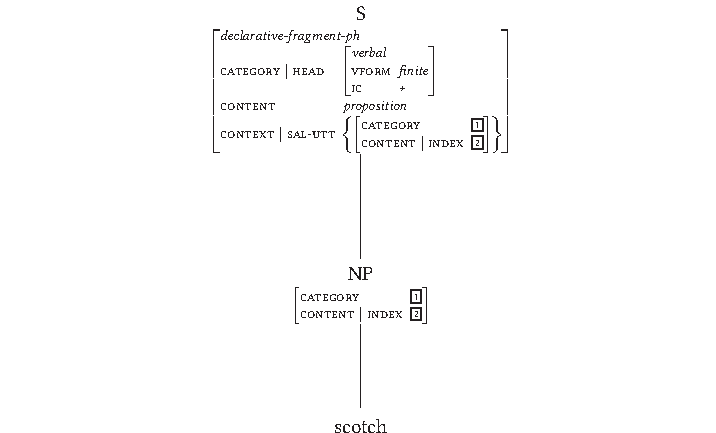
\includegraphics{figures/Ch1Fig5.pdf}
% \regAvmFonts\avmoptions{center}

% \newcommand{\AVMSfragment}{\begin{Avm}{S}
% 	\[\tp{declarative-fragment-ph}\\
% 	category \| head & \[\tp{verbal} \\ 
% 					 vform & finite\\
% 					 ic & +\]\\
%   content & proposition \\
  
%   context	\| sal-utt & \{\[category & \@{1}\\
%   											content \| index & \@{2}\]\}\]
%   \end{Avm}}

% \newcommand{\AVMNPfragment}{\begin{Avm}{NP}
% 	\[category & \@{1}\\
% 									content \| index & \@{2}\]
% 	\end{Avm}}
	

% \smallAvmFonts
% \begin{figure}[hbcd]
%   \begin{center}

% \begin{bundle}{\AVMSfragment}\setlength{\GapDepth}{50pt}
%                \chunk{\setlength{\GapDepth}{40pt}
%                   \begin{bundle}{\AVMNPfragment}
%                     \chunk{scotch}
%                   \end{bundle}}
             
%          \end{bundle}
% \regAvmFonts

\caption{Arbre simplifié de la phrase elliptique en \REF{ch1:ex143b}}
\label{ch1:fig5}
\end{figure}

Je reprends ici l’explication fournie par \citet[301]{GinzburgEtAl2000} par rapport au trait contextuel \is{Salient Utterance (SAL-UTT)}SAL-UTT : «~In information-structure terms, \is{Salient Utterance (SAL-UTT)}SAL-UTT can be thought of as means of underspecifying the subsequent focal (sub)utterance or as a potential parallel element in the sense of \citet{DalrympleEtAl1991} and \citet{Shieber1996}. [...] Which constituent of a given utterance will be the SAL-UTT need not be viewed as determined prior to that utterance’s taking place. Typically, the determination of SAL-UTT is a consequence of how conversationalist decides to structure her context, depending on which question she decides to make maximal in \is{Question Under Discussion (QUD)}QUD\footnote{QUD = \textit{Question Under Discussion}.} at a given point.~» 

L’identification de l’élément résiduel avec un corrélat approprié dans la phrase source, grâce au trait \is{Salient Utterance (SAL-UTT)}SAL-UTT, permet ainsi la \isi{reconstruction sémantique} du matériel manquant. Pour des détails supplémentaires, voir la section~\ref{ch2:sect2.5.3.2}.


\subsection{Quel type d’identité ?} \label{ch1:sect1.5.3}

Dans la section~\ref{ch1:sect1.3.3}, on a rapproché le phénomène de l’ellipse des relations \is{anaphore}anaphoriques, car de manière générale le matériel manquant doit être récupéré dans le contexte, à partir d’un antécédent dans le discours, comme c’est le cas des anaphores ordinaires.

La question qui se pose maintenant est quel type de relation s’établit entre le matériel manquant et son antécédent ? Bien que la réponse soit évidente après avoir énuméré les \isi{effets de connectivité} et surtout les effets de non-connectivité, je synthétise la discussion portée à ce sujet dans la littérature sur l’ellipse. 

Qu’on se situe dans une approche en termes de \isi{reconstruction syntaxique} ou bien dans une approche par \isi{reconstruction sémantique}, il semble que l’identité qui s’établit entre le matériel manquant et son antécédent est plutôt de nature sémantique. 

\subsubsection{Identité sémantique} 

Fondamentalement, le matériel manquant doit avoir la même interprétation que son antécédent (\citealt{DalrympleEtAl1991,Hardt1993,GinzburgEtAl2000,Merchant2001,CulicoverEtAl2005}, etc.). 

  
L’argument majeur pour postuler une identité sémantique regroupe tous les faits empiriques montrant des \is{asymétrie syntaxique}discordances entre la structure syntaxique de l’an\-técédent et celle du matériel manquant. La plupart d’entre eux ont été déjà discutés précédemment : les \is{asymétrie syntaxique}discordances de voix (cf. exemples \REF{ch1:ex130}), les violations des \isi{principes du liage} (cf. exemples \REF{ch1:ex132}, \REF{ch1:ex133} et \REF{ch1:ex134} ci-dessus), l’interprétation relâchée des pronoms \REF{ch1:ex122}, et on peut ajouter à cette liste le comportement des expressions de \isi{polarité}, cf. \citet{Sag1976}. En \REF{ch1:ex147}, on observe que l’indéfini se comporte comme un item de \isi{polarité} dans la phrase source, mais pas dans la phrase reconstruite. 

\ea
John didn’t see \textbf{anyone}, but Mary did. \citep[157]{Sag1976} \label{ch1:ex147}
\ea  ... but Mary did see \textbf{someone}. 
\ex  ... *but Mary did see \textbf{anyone}.
\z
\z

Un autre argument majeur en faveur de l’identité sémantique regroupe des faits liés à l’absence d’ambiguïté dans les contextes avec ellipse, alors que les mêmes structures sont par ailleurs ambiguës. Le premier type de contextes est représenté par les exemples en \REF{ch1:ex148}, toujours repris de \citet{Sag1976}. La séquence \textit{X is ready to eat} est a priori ambiguë entre une interprétation active (p.ex. \textit{X eats}) ou bien passive (p.ex. \textit{X is being eaten}). Pourtant, si cette séquence est suivie par une phrase elliptique, on observe que la phrase source et la phrase elliptique doivent avoir le même type d’interprétation (on obtient ainsi une interprétation parallèle dans les deux conjoints). La généralisation qui découle de ces exemples est la suivante : si plusieurs interprétations existent, la phrase elliptique doit recevoir la même interprétation que la phrase source.

\ea
The chickens are ready to eat and the children are, too. \citep[533]{Sag1976} \label{ch1:ex148}
\ea = The chickens eat and the children eat. 
\ex = The chickens are being eaten and the children are being eaten.
\ex ${\neq}$ The chickens eat and the children are being eaten.
\ex ${\neq}$ The chickens are being eaten and the children eat.
\z
\z

Le deuxième type d’exemples concerne la portée des quantifieurs. Dans la séquence \textit{Someone hit everyone} que représente la phrase source en \REF{ch1:ex149} reprise de \citet{Sag1976}, le quantifieur \textit{someone} peut avoir une \isi{portée large} ({\cad} quelqu’un a la propriété d’avoir frappé tout le monde) ou bien une \isi{portée étroite} ({\cad} tout le monde a été frappé par quelqu’un). Cependant, on observe que, bien que la phrase source permette les deux portées, la présence de la phrase elliptique enlève l’ambiguïté, le quantifieur \textit{someone} ne pouvant recevoir qu’une \isi{portée large}, car son corrélat dans la phrase elliptique (en l’occurrence, l’expression référentielle \textit{Bill}) n’a qu’une \isi{portée large}.

\ea
Someone hit everyone, and then Bill did. \citep[61]{Sag1976} \label{ch1:ex149} 
\z

Tous les faits mentionnés précédemment suggèrent que l’identité qui s’établit entre le matériel manquant et l’antécédent est essentiellement de nature sémantique. Dans la littérature, cette identité sémantique a été formalisée de différentes manières : (i) identité en forme logique, modulo le lambda-calcul (p.ex. \citealt{Sag1976,Williams1977})\footnote{Voir la notion \textit{alphabetic variance} de \citet{Sag1976}.}, ou (ii) identité de sens, modulo les éléments focalisés (p.ex. \citealt{Merchant2001,Merchant2004})\footnote{Voir la condition de \textit{e-givenness} de \citet{Merchant2001,Merchant2006} et l’implication mutuelle XP\textsubscript{A} {\textasciitilde} XP\textsubscript{E}.}.~


\subsubsection{Identité syntaxique}

Certains travaux issus des \is{approche structurale}approches structurales (p.ex. \citealt{Sag1976,Williams1977,FiengoEtAl1994,ChungEtAl1995}) postulent qu’entre le matériel manquant et l’antécédent on doit avoir une identité de structure syntaxique. 

Dans ces approches, l’identité syntaxique n’implique pas une identité «~superficielle~» (morpho-phonologique). Ainsi, dans les exemples en \REF{ch1:ex150} repris de \citet{Merchant2009}, on observe que les traits flexionnels ne sont pas pertinents : le matériel manquant peut correspondre à une forme verbale infinitive, alors que son antécédent est une forme fléchie au passé.

\ea \label{ch1:ex150}
\ea  Jake \textbf{ate} the sandwich even though his friend told him not \textbf{to} {\textless}\textbf{eat} the sandwich{\textgreater}. 
\ex  Emily \textbf{played} beautifully at the recital and her sister \textbf{will} too {\textless}\textbf{play} beautifully at the recital{\textgreater}.  
\z
\z

Parmi les arguments invoqués en faveur de ce type d'approches, on mentionne le comportement spécial de l’auxiliaire \textit{be} en anglais (cf. \citealt{Merchant2009}). Contrairement aux autres verbes de l’anglais, l’auxiliaire \textit{be} exige une identité morphologique dans les constructions elliptiques : un exemple avec \textit{be} en \REF{ch1:ex151}, bien que construit de la même façon que \REF{ch1:ex150}, est agrammatical ; le matériel manquant comportant cet auxiliaire doit avoir la même forme morphologique que son antécédent.

\ea \label{ch1:ex151}
*Emily \textbf{was} beautiful at the recital and her sister \textbf{will} too {\textless}\textbf{be} beautiful at the recital{\textgreater}.   
\z

\citeauthor{Merchant2008a} (\citeyear*{Merchant2008a,Merchant2009}) ajoute, comme possible argument, la distribution asy\-métrique des \is{asymétrie syntaxique}discordances de voix dans les \is{high ellipsis}ellipses «~hautes~» par rapport aux \is{low ellipsis}ellipses «~basses~» (angl. \textit{high vs. low ellipsis}). Il observe que~dans les ellipses qu’il appelle \is{high ellipsis}«~hautes~» (p.ex. \is{Sluicing}sluicing, gapping, \is{Stripping}stripping, \is{réponse courte}réponses courtes), l’antécédent et le matériel manquant doivent partager la même voix, ce qui explique l’agrammaticalité des exemples \REF{ch1:ex152a} et \REF{ch1:ex153a}. En revanche, dans les \is{low ellipsis}ellipses «~basses~» (p.ex. \is{Verb Phrase Ellipsis (VPE)}VPE ou \is{Pseudogapping}pseudogapping), on peut avoir des \is{asymétrie syntaxique}discordances de voix entre le matériel manquant et son antécédent : le matériel manquant peut avoir une forme active et son antécédent une forme passive \REF{ch1:ex152b}, et vice-versa \REF{ch1:ex153b}. Merchant explique cette distribution irrégulière en termes d’identité syntaxique : les \is{high ellipsis}ellipses «~hautes~», élidant plus que le simple syntagme verbal (angl. VP), sont sensibles à la présence du nœud Voix (angl. \textit{Voice}) qu’elles incluent et exigent donc des traits de Voix identiques, alors que dans le cas des \is{low ellipsis}ellipses «~basses~», le nœud Voix se trouve à l’extérieur du matériel effacé (car l’ellipse du syntagme verbal ne l’inclut pas), donc la Voix n’a aucune incidence sur les conditions d’identité\footnote{Il faut noter cependant que ces \is{asymétrie syntaxique}asymétries de voix ont reçu aussi d’autres explications. Voir l’explication en termes de \isi{processing}, donnée par \citet{FrazierEtAl2005,FrazierEtAl2006}, ou encore l’explication en termes de relations de \isi{cohérence discursive}, donnée par \citet{Kehler2000,Kehler2002}.}. La conclusion de Merchant est la suivante : A chaque fois qu’il y a une discordance apparente, le déclencheur de l’ellipse se situe en dehors du site de l’ellipse, alors que la cible se trouve à l’intérieur.

\ea
\ea  *Joe \textbf{was murdered}, but we don’t know who {\textless}\textbf{murdered} Joe{\textgreater}. \label{ch1:ex152a}
\ex  This problem \textbf{was} \textbf{to have been looked} into, but obviously nobody \textbf{did} {\textless}\textbf{look} into this problem{\textgreater}. \label{ch1:ex152b}
\z
\z

\ea
\ea  *Someone \textbf{murdered} Joe, but we don’t know who by {\textless}Joe \textbf{was murdered}{\textgreater}. \label{ch1:ex153a}
\ex  The janitor should \textbf{remove} the trash whenever it is apparent that it needs to \textbf{be} {\textless}\textbf{removed}{\textgreater}. \label{ch1:ex153b}
\z
\z

Un autre fait soutenant (au moins dans certains contextes) une identité syntaxique est lié au comportement des éléments résiduels qui peuvent être marqués par une préposition dans les constructions avec \is{Sluicing}sluicing. \citet{Chung2005} observe qu’un argument marqué habituellement par une préposition (comme c’est le cas du syntagme prépositionnel \textit{about what} en \REF{ch1:ex154}) peut apparaître sans préposition uniquement s’il a un corrélat explicite dans la phrase source \REF{ch1:ex154c} ; si son corrélat est implicite, l’élément résiduel doit comporter la préposition (comparer \REF{ch1:ex154a} et \REF{ch1:ex154b}). \citet{Chung2005} ajoute donc pour le \is{Sluicing}sluicing une contrainte lexico-syntaxique concernant l’identité qui doit s’établir entre le matériel manquant et son antécédent : chaque élément appartenant au matériel manquant doit avoir un corrélat lexical dans l’antécédent de la phrase source (contrainte résumée en anglais comme : \textit{no new words}). 

\ea \label{ch1:ex154}
\ea  Bill is upset. Guess about what {\textless}he’s upset{\textgreater}. \label{ch1:ex154a} 
\ex  Bill is upset. *Guess what {\textless}he’s upset about{\textgreater}. \label{ch1:ex154b}
\ex  Bill is upset about something. Guess what {\textless}he’s upset about{\textgreater}. \label{ch1:ex154c} 
\z
\z

Toujours dans les constructions avec \is{Sluicing}sluicing, on note (cf. \citealt{Merchant2013b}) l’absence des alternances de valence (\ref{ch1:ex155c}--\ref{ch1:ex155d}), bien que l’alter\-nance de position des objets soit possible en dehors de l’ellipse (\ref{ch1:ex155a}--\ref{ch1:ex155b}).

\ea
\ea  They embroidered [something] [\textbf{with} peace signs]. \citep[99]{Merchant2013b} \label{ch1:ex155a} 
\ex  They embroidered [peace signs] [\textbf{on} something]. \label{ch1:ex155b}
\ex  *They embroidered [something] [\textbf{with} peace signs], but I don’t know what \textbf{on}. \label{ch1:ex155c}
\ex  *They embroidered [something] [\textbf{on} their jackets], but I don’t know \textbf{with} what. \label{ch1:ex155d}
\z
\z

Enfin, on doit ajouter le fait qu’il y a des approches postulant une identité hybride (p.ex. \citealt{Kehler2002}) : le matériel manquant et l’antécédent sont identiques tant au niveau sémantique que syntaxique. 


\section{Conclusion}

Dans ce chapitre, j’ai donné un aperçu de la problématique de l’ellipse, phéno\-mène qui sera étudié dans les chapitres suivants à travers deux constructions : (i) le gapping dans la coordination, et (ii) les relatives partitives sans verbe dans le domaine de la subordination. 

Pour pouvoir parler d’ellipse dans une structure, il faut~(i) qu’une partie du matériel nécessaire à l’interprétation manque dans la structure syntaxique, et (ii) que le matériel manquant soit récupérable à partir d’un antécédent dans le contexte (linguistique ou extra-linguistique). Contrairement à ce que l’on peut croire, l’ellipse n’est pas toujours facultative ; par conséquent, on ne peut pas réduire tous les emplois de l’ellipse au principe du moindre effort.  

Traditionnellement, la phrase «~complète~» est considérée comme étant la phrase qui contient une tête verbale à un mode personnel. J’ai montré, en m’appu\-yant sur les données du roumain et du français, qu’on peut avoir des phrases «~complètes~» avec des formes verbales non finies ou encore des phrases «~complètes~» \is{phrase averbale}averbales, dont la tête n’est pas un verbe. Contrairement aux phrases complètes, les phrases elliptiques ont une constituance «~incomplète~» et n’ont pas d’autono\-mie discursive.

J’ai fait ensuite l’inventaire des constructions elliptiques majeures, en fonction de trois critères : la nature du matériel manquant, le type de contexte syntaxique dans lequel apparaît le type d’ellipse en question et la directionnalité de l’ellipse. En ce qui concerne les conditions de légitimité de l’ellipse, on observe que (i) chaque type d’ellipse est autorisé dans un certain type de configuration syntaxique, et que (ii) tous les types d’ellipse n’apparaissent pas dans toutes les langues. On a vu que l’identification des différentes constructions est un travail difficile si l’on se place dans une perspective typologique.  

Pour ce qui est de la résolution de l’ellipse ({\cad} le moyen mis en place pour récupérer l’information qui manque), on a vu que plusieurs possibilités d’analyse se présentent, en fonction du niveau linguistique auquel opère la résolution, {\cad} la syntaxe, la sémantique ou bien l’interface syntaxe-sémantique. Les propositions se regroupent en deux approches majeures, que j’ai appelées, en suivant \citet{Merchant2009}, \is{approche structurale}approches structurales vs. \is{approche non structurale}approches non structurales. Le choix entre l’une ou l’autre de ces approches joue autour des \isi{effets de connectivité} ou de non-connectivité, qu’on observe entre la phrase source et la phrase elliptique : l’ellipse syntaxique semble être justifiée à chaque fois qu’on observe des \isi{effets de connectivité}, alors que l’ellipse sémantique semble être plus attractive dans les situations qui ne présentent pas ces effets. Au-delà de la compétition existant entre ces deux approches pour expliquer un même phénomène elliptique, je considère que dans une grammaire de l’ellipse les deux solutions doivent être disponibles, car on ne peut pas établir d’analyse uniforme pour toutes les constructions elliptiques d’une langue (voir aussi \citealt{GinzburgEtAlToAppear}) et parfois on ne peut pas avoir une analyse unitaire même pour une même construction elliptique dans des langues différentes. La description et l’analyse de l’ellipse doivent se faire donc construction par construction et langue par langue.

Bien que les constructions elliptiques dans leur hétérogénéité obéissent à des contraintes grammaticales plus ou moins strictes, la contrainte majeure s’appli\-quant à toutes les constructions elliptiques~concerne l’identité sémantique qui doit caractériser la relation entre le matériel manquant et son antécédent ({\cad} ils doivent être équivalents quant à leurs conditions de vérité). 

Dans l’étude du phénomène de l’ellipse, j’ai pris en compte surtout les facteurs syntaxiques et sémantiques. Des travaux récents, que je n’ai pas présentés dans ce chapitre, révèlent l’importance d’autres types de facteurs dans le fonctionnement de l’ellipse : la \isi{structure informationnelle} (p.ex. \citealt{Winkler2005,Kertz2010,Kertz2013}), les relations de \isi{cohérence discursive} (p.ex. \citealt{Kehler1994,Kehler2000,Kehler2002}) ou encore les facteurs psycholinguistiques (p.ex. \citealt{Carlson2001,Carlson2002,CarlsonEtAl2005,MartinEtAl2009,MartinEtAl2011,YoshidaEtAl2012}). 


